% ------------------------------------------------------------------------------------------------------------------
% Basic configuration and packages
% ------------------------------------------------------------------------------------------------------------------
% Package for discovering wrong and outdated usage of LaTeX.
% More information to be found in l2tabu English version.
\RequirePackage[l2tabu, orthodox]{nag}
% Class of LaTeX document: {size of paper, size of font}[document class]
\documentclass[a4paper,11pt]{article}



% ------------------------------------------------------
% Packages not tied to particular normal language
% ------------------------------------------------------
% This package should improved spaces in the text
\usepackage{microtype}
% Add few important symbols, like text Celcius degree
\usepackage{textcomp}



% ------------------------------------------------------
% Polonization of LaTeX document
% ------------------------------------------------------
% Basic polonization of the text
\usepackage[MeX]{polski}
% Switching on UTF-8 encoding
\usepackage[utf8]{inputenc}
% Adding font Latin Modern
\usepackage{lmodern}
% Package is need for fonts Latin Modern
\usepackage[T1]{fontenc}



% ------------------------------------------------------
% Setting margins
% ------------------------------------------------------
\usepackage[a4paper, total={14cm, 25cm}]{geometry}



% ------------------------------------------------------
% Setting vertical spaces in the text
% ------------------------------------------------------
% Setting space between lines
\renewcommand{\baselinestretch}{1.1}

% Setting space between lines in tables
\renewcommand{\arraystretch}{1.4}



% ------------------------------------------------------
% Packages for scientific papers
% ------------------------------------------------------
% Switching off \lll symbol, that I guess is representing letter "Ł"
% It collide with `amsmath' package's command with the same name
\let\lll\undefined
% Basic package from American Mathematical Society (AMS)
\usepackage[intlimits]{amsmath}
% Equations are numbered separately in every section
\numberwithin{equation}{section}

% Other very useful packages from AMS
\usepackage{amsfonts}
\usepackage{amssymb}
\usepackage{amscd}
\usepackage{amsthm}

% Package with better looking calligraphy fonts
\usepackage{calrsfs}

% Package with better looking greek letters
% Example of use: pi -> \uppi
\usepackage{upgreek}
% Improving look of lambda letter
\let\oldlambda\lambda
\renewcommand{\lambda}{\uplambda}




% ------------------------------------------------------
% BibLaTeX
% ------------------------------------------------------
% Package biblatex, with biber as its backend, allow us to handle
% bibliography entries that use Unicode symbols outside ASCII
% \usepackage[
% language=polish,
% backend=biber,
% style=alphabetic,
% url=false,
% eprint=true,
% ]{biblatex}

% \addbibresource{Logika-i-teoria-mnogości-Bibliography.bib}





% ------------------------------------------------------
% Defining new environments (?)
% ------------------------------------------------------
% Defining enviroment "Wniosek"
% \newtheorem{corollary}{Wniosek}
% \newtheorem{definition}{Definicja}
% \newtheorem{theorem}{Twierdzenie}





% ------------------------------------------------------
% xcolor, the main LaTeX color package
% ------------------------------------------------------

\usepackage{xcolor}

% Defining colors in RGB system
\definecolor{colorR5G130B0}{RGB}{5, 130, 0}
\definecolor{colorR10G130B0}{RGB}{10, 130, 0}
\definecolor{colorR15G130B0}{RGB}{15, 130, 0}
\definecolor{colorR20G130B0}{RGB}{20, 130, 0}
\definecolor{colorR25G130B0}{RGB}{25, 130, 0}
\definecolor{colorR30G130B0}{RGB}{30, 130, 0}
\definecolor{colorR35G130B0}{RGB}{35, 130, 0}
\definecolor{colorR40G130B0}{RGB}{40, 130, 0}
\definecolor{colorR45G130B0}{RGB}{45, 130, 0}
\definecolor{colorR50G130B0}{RGB}{50, 130, 0}
\definecolor{colorR55G130B0}{RGB}{55, 130, 0}
\definecolor{colorR60G130B0}{RGB}{60, 130, 0}
\definecolor{colorR65G130B0}{RGB}{65, 130, 0}
\definecolor{colorR70G130B0}{RGB}{70, 130, 0}
\definecolor{colorR75G130B0}{RGB}{75, 130, 0}
\definecolor{colorR80G130B0}{RGB}{80, 130, 0}
\definecolor{colorR85G130B0}{RGB}{85, 130, 0}
\definecolor{colorR90G130B0}{RGB}{90, 130, 0}
\definecolor{colorR95G130B0}{RGB}{95, 130, 0}
\definecolor{colorR100G130B0}{RGB}{100, 130, 0}
\definecolor{colorR105G130B0}{RGB}{105, 130, 0}
\definecolor{colorR110G130B0}{RGB}{110, 130, 0}
\definecolor{colorR115G130B0}{RGB}{115, 130, 0}
\definecolor{colorR120G130B0}{RGB}{120, 130, 0}
\definecolor{colorR125G130B0}{RGB}{125, 130, 0}
\definecolor{colorR130G130B0}{RGB}{130, 130, 0}
\definecolor{colorR135G130B0}{RGB}{135, 130, 0}
\definecolor{colorR140G130B0}{RGB}{140, 130, 0}
\definecolor{colorR145G130B0}{RGB}{145, 130, 0}
\definecolor{colorR150G130B0}{RGB}{150, 130, 0}
\definecolor{colorR155G130B0}{RGB}{155, 130, 0}
\definecolor{colorR160G130B0}{RGB}{160, 130, 0}
\definecolor{colorR165G130B0}{RGB}{165, 130, 0}
\definecolor{colorR170G130B0}{RGB}{170, 130, 0}
\definecolor{colorR175G130B0}{RGB}{175, 130, 0}
\definecolor{colorR180G130B0}{RGB}{180, 130, 0}
\definecolor{colorR185G130B0}{RGB}{185, 130, 0}
\definecolor{colorR190G130B0}{RGB}{190, 130, 0}
\definecolor{colorR195G130B0}{RGB}{195, 130, 0}
\definecolor{colorR200G130B0}{RGB}{200, 130, 0}
\definecolor{colorR205G130B0}{RGB}{205, 130, 0}
\definecolor{colorR210G130B0}{RGB}{210, 130, 0}
\definecolor{colorR215G130B0}{RGB}{215, 130, 0}
\definecolor{colorR220G130B0}{RGB}{220, 130, 0}
\definecolor{colorR225G130B0}{RGB}{225, 130, 0}
\definecolor{colorR230G130B0}{RGB}{230, 130, 0}
\definecolor{colorR235G130B0}{RGB}{235, 130, 0}
\definecolor{colorR240G130B0}{RGB}{240, 130, 0}
\definecolor{colorR245G130B0}{RGB}{245, 130, 0}
\definecolor{colorR250G130B0}{RGB}{250, 130, 0}
\definecolor{colorR255G130B0}{RGB}{255, 130, 0}

\definecolor{colorR5G135B0}{RGB}{5, 135, 0}
\definecolor{colorR10G135B0}{RGB}{10, 135, 0}
\definecolor{colorR15G135B0}{RGB}{15, 135, 0}
\definecolor{colorR20G135B0}{RGB}{20, 135, 0}
\definecolor{colorR25G135B0}{RGB}{25, 135, 0}
\definecolor{colorR30G135B0}{RGB}{30, 135, 0}
\definecolor{colorR35G135B0}{RGB}{35, 135, 0}
\definecolor{colorR40G135B0}{RGB}{40, 135, 0}
\definecolor{colorR45G135B0}{RGB}{45, 135, 0}
\definecolor{colorR50G135B0}{RGB}{50, 135, 0}
\definecolor{colorR55G135B0}{RGB}{55, 135, 0}
\definecolor{colorR60G135B0}{RGB}{60, 135, 0}
\definecolor{colorR65G135B0}{RGB}{65, 135, 0}
\definecolor{colorR70G135B0}{RGB}{70, 135, 0}
\definecolor{colorR75G135B0}{RGB}{75, 135, 0}
\definecolor{colorR80G135B0}{RGB}{80, 135, 0}
\definecolor{colorR85G135B0}{RGB}{85, 135, 0}
\definecolor{colorR90G135B0}{RGB}{90, 135, 0}
\definecolor{colorR95G135B0}{RGB}{95, 135, 0}
\definecolor{colorR100G135B0}{RGB}{100, 135, 0}
\definecolor{colorR105G135B0}{RGB}{105, 135, 0}
\definecolor{colorR110G135B0}{RGB}{110, 135, 0}
\definecolor{colorR115G135B0}{RGB}{115, 135, 0}
\definecolor{colorR120G135B0}{RGB}{120, 135, 0}
\definecolor{colorR125G135B0}{RGB}{125, 135, 0}
\definecolor{colorR130G135B0}{RGB}{130, 135, 0}
\definecolor{colorR135G135B0}{RGB}{135, 135, 0}
\definecolor{colorR140G135B0}{RGB}{140, 135, 0}
\definecolor{colorR145G135B0}{RGB}{145, 135, 0}
\definecolor{colorR150G135B0}{RGB}{150, 135, 0}
\definecolor{colorR155G135B0}{RGB}{155, 135, 0}
\definecolor{colorR160G135B0}{RGB}{160, 135, 0}
\definecolor{colorR165G135B0}{RGB}{165, 135, 0}
\definecolor{colorR170G135B0}{RGB}{170, 135, 0}
\definecolor{colorR175G135B0}{RGB}{175, 135, 0}
\definecolor{colorR180G135B0}{RGB}{180, 135, 0}
\definecolor{colorR185G135B0}{RGB}{185, 135, 0}
\definecolor{colorR190G135B0}{RGB}{190, 135, 0}
\definecolor{colorR195G135B0}{RGB}{195, 135, 0}
\definecolor{colorR200G135B0}{RGB}{200, 135, 0}
\definecolor{colorR205G135B0}{RGB}{205, 135, 0}
\definecolor{colorR210G135B0}{RGB}{210, 135, 0}
\definecolor{colorR215G135B0}{RGB}{215, 135, 0}
\definecolor{colorR220G135B0}{RGB}{220, 135, 0}
\definecolor{colorR225G135B0}{RGB}{225, 135, 0}
\definecolor{colorR230G135B0}{RGB}{230, 135, 0}
\definecolor{colorR235G135B0}{RGB}{235, 135, 0}
\definecolor{colorR240G135B0}{RGB}{240, 135, 0}
\definecolor{colorR245G135B0}{RGB}{245, 135, 0}
\definecolor{colorR250G135B0}{RGB}{250, 135, 0}
\definecolor{colorR255G135B0}{RGB}{255, 135, 0}

\definecolor{colorR5G140B0}{RGB}{5, 140, 0}
\definecolor{colorR10G140B0}{RGB}{10, 140, 0}
\definecolor{colorR15G140B0}{RGB}{15, 140, 0}
\definecolor{colorR20G140B0}{RGB}{20, 140, 0}
\definecolor{colorR25G140B0}{RGB}{25, 140, 0}
\definecolor{colorR30G140B0}{RGB}{30, 140, 0}
\definecolor{colorR35G140B0}{RGB}{35, 140, 0}
\definecolor{colorR40G140B0}{RGB}{40, 140, 0}
\definecolor{colorR45G140B0}{RGB}{45, 140, 0}
\definecolor{colorR50G140B0}{RGB}{50, 140, 0}
\definecolor{colorR55G140B0}{RGB}{55, 140, 0}
\definecolor{colorR60G140B0}{RGB}{60, 140, 0}
\definecolor{colorR65G140B0}{RGB}{65, 140, 0}
\definecolor{colorR70G140B0}{RGB}{70, 140, 0}
\definecolor{colorR75G140B0}{RGB}{75, 140, 0}
\definecolor{colorR80G140B0}{RGB}{80, 140, 0}
\definecolor{colorR85G140B0}{RGB}{85, 140, 0}
\definecolor{colorR90G140B0}{RGB}{90, 140, 0}
\definecolor{colorR95G140B0}{RGB}{95, 140, 0}
\definecolor{colorR100G140B0}{RGB}{100, 140, 0}
\definecolor{colorR105G140B0}{RGB}{105, 140, 0}
\definecolor{colorR110G140B0}{RGB}{110, 140, 0}
\definecolor{colorR115G140B0}{RGB}{115, 140, 0}
\definecolor{colorR120G140B0}{RGB}{120, 140, 0}
\definecolor{colorR125G140B0}{RGB}{125, 140, 0}
\definecolor{colorR130G140B0}{RGB}{130, 140, 0}
\definecolor{colorR135G140B0}{RGB}{135, 140, 0}
\definecolor{colorR140G140B0}{RGB}{140, 140, 0}
\definecolor{colorR145G140B0}{RGB}{145, 140, 0}
\definecolor{colorR150G140B0}{RGB}{150, 140, 0}
\definecolor{colorR155G140B0}{RGB}{155, 140, 0}
\definecolor{colorR160G140B0}{RGB}{160, 140, 0}
\definecolor{colorR165G140B0}{RGB}{165, 140, 0}
\definecolor{colorR170G140B0}{RGB}{170, 140, 0}
\definecolor{colorR175G140B0}{RGB}{175, 140, 0}
\definecolor{colorR180G140B0}{RGB}{180, 140, 0}
\definecolor{colorR185G140B0}{RGB}{185, 140, 0}
\definecolor{colorR190G140B0}{RGB}{190, 140, 0}
\definecolor{colorR195G140B0}{RGB}{195, 140, 0}
\definecolor{colorR200G140B0}{RGB}{200, 140, 0}
\definecolor{colorR205G140B0}{RGB}{205, 140, 0}
\definecolor{colorR210G140B0}{RGB}{210, 140, 0}
\definecolor{colorR215G140B0}{RGB}{215, 140, 0}
\definecolor{colorR220G140B0}{RGB}{220, 140, 0}
\definecolor{colorR225G140B0}{RGB}{225, 140, 0}
\definecolor{colorR230G140B0}{RGB}{230, 140, 0}
\definecolor{colorR235G140B0}{RGB}{235, 140, 0}
\definecolor{colorR240G140B0}{RGB}{240, 140, 0}
\definecolor{colorR245G140B0}{RGB}{245, 140, 0}
\definecolor{colorR250G140B0}{RGB}{250, 140, 0}
\definecolor{colorR255G140B0}{RGB}{255, 140, 0}

\definecolor{colorR5G145B0}{RGB}{5, 145, 0}
\definecolor{colorR10G145B0}{RGB}{10, 145, 0}
\definecolor{colorR15G145B0}{RGB}{15, 145, 0}
\definecolor{colorR20G145B0}{RGB}{20, 145, 0}
\definecolor{colorR25G145B0}{RGB}{25, 145, 0}
\definecolor{colorR30G145B0}{RGB}{30, 145, 0}
\definecolor{colorR35G145B0}{RGB}{35, 145, 0}
\definecolor{colorR40G145B0}{RGB}{40, 145, 0}
\definecolor{colorR45G145B0}{RGB}{45, 145, 0}
\definecolor{colorR50G145B0}{RGB}{50, 145, 0}
\definecolor{colorR55G145B0}{RGB}{55, 145, 0}
\definecolor{colorR60G145B0}{RGB}{60, 145, 0}
\definecolor{colorR65G145B0}{RGB}{65, 145, 0}
\definecolor{colorR70G145B0}{RGB}{70, 145, 0}
\definecolor{colorR75G145B0}{RGB}{75, 145, 0}
\definecolor{colorR80G145B0}{RGB}{80, 145, 0}
\definecolor{colorR85G145B0}{RGB}{85, 145, 0}
\definecolor{colorR90G145B0}{RGB}{90, 145, 0}
\definecolor{colorR95G145B0}{RGB}{95, 145, 0}
\definecolor{colorR100G145B0}{RGB}{100, 145, 0}
\definecolor{colorR105G145B0}{RGB}{105, 145, 0}
\definecolor{colorR110G145B0}{RGB}{110, 145, 0}
\definecolor{colorR115G145B0}{RGB}{115, 145, 0}
\definecolor{colorR120G145B0}{RGB}{120, 145, 0}
\definecolor{colorR125G145B0}{RGB}{125, 145, 0}
\definecolor{colorR130G145B0}{RGB}{130, 145, 0}
\definecolor{colorR135G145B0}{RGB}{135, 145, 0}
\definecolor{colorR140G145B0}{RGB}{140, 145, 0}
\definecolor{colorR145G145B0}{RGB}{145, 145, 0}
\definecolor{colorR150G145B0}{RGB}{150, 145, 0}
\definecolor{colorR155G145B0}{RGB}{155, 145, 0}
\definecolor{colorR160G145B0}{RGB}{160, 145, 0}
\definecolor{colorR165G145B0}{RGB}{165, 145, 0}
\definecolor{colorR170G145B0}{RGB}{170, 145, 0}
\definecolor{colorR175G145B0}{RGB}{175, 145, 0}
\definecolor{colorR180G145B0}{RGB}{180, 145, 0}
\definecolor{colorR185G145B0}{RGB}{185, 145, 0}
\definecolor{colorR190G145B0}{RGB}{190, 145, 0}
\definecolor{colorR195G145B0}{RGB}{195, 145, 0}
\definecolor{colorR200G145B0}{RGB}{200, 145, 0}
\definecolor{colorR205G145B0}{RGB}{205, 145, 0}
\definecolor{colorR210G145B0}{RGB}{210, 145, 0}
\definecolor{colorR215G145B0}{RGB}{215, 145, 0}
\definecolor{colorR220G145B0}{RGB}{220, 145, 0}
\definecolor{colorR225G145B0}{RGB}{225, 145, 0}
\definecolor{colorR230G145B0}{RGB}{230, 145, 0}
\definecolor{colorR235G145B0}{RGB}{235, 145, 0}
\definecolor{colorR240G145B0}{RGB}{240, 145, 0}
\definecolor{colorR245G145B0}{RGB}{245, 145, 0}
\definecolor{colorR250G145B0}{RGB}{250, 145, 0}
\definecolor{colorR255G145B0}{RGB}{255, 145, 0}

\definecolor{colorR5G150B0}{RGB}{5, 150, 0}
\definecolor{colorR10G150B0}{RGB}{10, 150, 0}
\definecolor{colorR15G150B0}{RGB}{15, 150, 0}
\definecolor{colorR20G150B0}{RGB}{20, 150, 0}
\definecolor{colorR25G150B0}{RGB}{25, 150, 0}
\definecolor{colorR30G150B0}{RGB}{30, 150, 0}
\definecolor{colorR35G150B0}{RGB}{35, 150, 0}
\definecolor{colorR40G150B0}{RGB}{40, 150, 0}
\definecolor{colorR45G150B0}{RGB}{45, 150, 0}
\definecolor{colorR50G150B0}{RGB}{50, 150, 0}
\definecolor{colorR55G150B0}{RGB}{55, 150, 0}
\definecolor{colorR60G150B0}{RGB}{60, 150, 0}
\definecolor{colorR65G150B0}{RGB}{65, 150, 0}
\definecolor{colorR70G150B0}{RGB}{70, 150, 0}
\definecolor{colorR75G150B0}{RGB}{75, 150, 0}
\definecolor{colorR80G150B0}{RGB}{80, 150, 0}
\definecolor{colorR85G150B0}{RGB}{85, 150, 0}
\definecolor{colorR90G150B0}{RGB}{90, 150, 0}
\definecolor{colorR95G150B0}{RGB}{95, 150, 0}
\definecolor{colorR100G150B0}{RGB}{100, 150, 0}
\definecolor{colorR105G150B0}{RGB}{105, 150, 0}
\definecolor{colorR110G150B0}{RGB}{110, 150, 0}
\definecolor{colorR115G150B0}{RGB}{115, 150, 0}
\definecolor{colorR120G150B0}{RGB}{120, 150, 0}
\definecolor{colorR125G150B0}{RGB}{125, 150, 0}
\definecolor{colorR130G150B0}{RGB}{130, 150, 0}
\definecolor{colorR135G150B0}{RGB}{135, 150, 0}
\definecolor{colorR140G150B0}{RGB}{140, 150, 0}
\definecolor{colorR145G150B0}{RGB}{145, 150, 0}
\definecolor{colorR150G150B0}{RGB}{150, 150, 0}
\definecolor{colorR155G150B0}{RGB}{155, 150, 0}
\definecolor{colorR160G150B0}{RGB}{160, 150, 0}
\definecolor{colorR165G150B0}{RGB}{165, 150, 0}
\definecolor{colorR170G150B0}{RGB}{170, 150, 0}
\definecolor{colorR175G150B0}{RGB}{175, 150, 0}
\definecolor{colorR180G150B0}{RGB}{180, 150, 0}
\definecolor{colorR185G150B0}{RGB}{185, 150, 0}
\definecolor{colorR190G150B0}{RGB}{190, 150, 0}
\definecolor{colorR195G150B0}{RGB}{195, 150, 0}
\definecolor{colorR200G150B0}{RGB}{200, 150, 0}
\definecolor{colorR205G150B0}{RGB}{205, 150, 0}
\definecolor{colorR210G150B0}{RGB}{210, 150, 0}
\definecolor{colorR215G150B0}{RGB}{215, 150, 0}
\definecolor{colorR220G150B0}{RGB}{220, 150, 0}
\definecolor{colorR225G150B0}{RGB}{225, 150, 0}
\definecolor{colorR230G150B0}{RGB}{230, 150, 0}
\definecolor{colorR235G150B0}{RGB}{235, 150, 0}
\definecolor{colorR240G150B0}{RGB}{240, 150, 0}
\definecolor{colorR245G150B0}{RGB}{245, 150, 0}
\definecolor{colorR250G150B0}{RGB}{250, 150, 0}
\definecolor{colorR255G150B0}{RGB}{255, 150, 0}

\definecolor{colorR5G155B0}{RGB}{5, 155, 0}
\definecolor{colorR10G155B0}{RGB}{10, 155, 0}
\definecolor{colorR15G155B0}{RGB}{15, 155, 0}
\definecolor{colorR20G155B0}{RGB}{20, 155, 0}
\definecolor{colorR25G155B0}{RGB}{25, 155, 0}
\definecolor{colorR30G155B0}{RGB}{30, 155, 0}
\definecolor{colorR35G155B0}{RGB}{35, 155, 0}
\definecolor{colorR40G155B0}{RGB}{40, 155, 0}
\definecolor{colorR45G155B0}{RGB}{45, 155, 0}
\definecolor{colorR50G155B0}{RGB}{50, 155, 0}
\definecolor{colorR55G155B0}{RGB}{55, 155, 0}
\definecolor{colorR60G155B0}{RGB}{60, 155, 0}
\definecolor{colorR65G155B0}{RGB}{65, 155, 0}
\definecolor{colorR70G155B0}{RGB}{70, 155, 0}
\definecolor{colorR75G155B0}{RGB}{75, 155, 0}
\definecolor{colorR80G155B0}{RGB}{80, 155, 0}
\definecolor{colorR85G155B0}{RGB}{85, 155, 0}
\definecolor{colorR90G155B0}{RGB}{90, 155, 0}
\definecolor{colorR95G155B0}{RGB}{95, 155, 0}
\definecolor{colorR100G155B0}{RGB}{100, 155, 0}
\definecolor{colorR105G155B0}{RGB}{105, 155, 0}
\definecolor{colorR110G155B0}{RGB}{110, 155, 0}
\definecolor{colorR115G155B0}{RGB}{115, 155, 0}
\definecolor{colorR120G155B0}{RGB}{120, 155, 0}
\definecolor{colorR125G155B0}{RGB}{125, 155, 0}
\definecolor{colorR130G155B0}{RGB}{130, 155, 0}
\definecolor{colorR135G155B0}{RGB}{135, 155, 0}
\definecolor{colorR140G155B0}{RGB}{140, 155, 0}
\definecolor{colorR145G155B0}{RGB}{145, 155, 0}
\definecolor{colorR150G155B0}{RGB}{150, 155, 0}
\definecolor{colorR155G155B0}{RGB}{155, 155, 0}
\definecolor{colorR160G155B0}{RGB}{160, 155, 0}
\definecolor{colorR165G155B0}{RGB}{165, 155, 0}
\definecolor{colorR170G155B0}{RGB}{170, 155, 0}
\definecolor{colorR175G155B0}{RGB}{175, 155, 0}
\definecolor{colorR180G155B0}{RGB}{180, 155, 0}
\definecolor{colorR185G155B0}{RGB}{185, 155, 0}
\definecolor{colorR190G155B0}{RGB}{190, 155, 0}
\definecolor{colorR195G155B0}{RGB}{195, 155, 0}
\definecolor{colorR200G155B0}{RGB}{200, 155, 0}
\definecolor{colorR205G155B0}{RGB}{205, 155, 0}
\definecolor{colorR210G155B0}{RGB}{210, 155, 0}
\definecolor{colorR215G155B0}{RGB}{215, 155, 0}
\definecolor{colorR220G155B0}{RGB}{220, 155, 0}
\definecolor{colorR225G155B0}{RGB}{225, 155, 0}
\definecolor{colorR230G155B0}{RGB}{230, 155, 0}
\definecolor{colorR235G155B0}{RGB}{235, 155, 0}
\definecolor{colorR240G155B0}{RGB}{240, 155, 0}
\definecolor{colorR245G155B0}{RGB}{245, 155, 0}
\definecolor{colorR250G155B0}{RGB}{250, 155, 0}
\definecolor{colorR255G155B0}{RGB}{255, 155, 0}

\definecolor{colorR5G160B0}{RGB}{5, 160, 0}
\definecolor{colorR10G160B0}{RGB}{10, 160, 0}
\definecolor{colorR15G160B0}{RGB}{15, 160, 0}
\definecolor{colorR20G160B0}{RGB}{20, 160, 0}
\definecolor{colorR25G160B0}{RGB}{25, 160, 0}
\definecolor{colorR30G160B0}{RGB}{30, 160, 0}
\definecolor{colorR35G160B0}{RGB}{35, 160, 0}
\definecolor{colorR40G160B0}{RGB}{40, 160, 0}
\definecolor{colorR45G160B0}{RGB}{45, 160, 0}
\definecolor{colorR50G160B0}{RGB}{50, 160, 0}
\definecolor{colorR55G160B0}{RGB}{55, 160, 0}
\definecolor{colorR60G160B0}{RGB}{60, 160, 0}
\definecolor{colorR65G160B0}{RGB}{65, 160, 0}
\definecolor{colorR70G160B0}{RGB}{70, 160, 0}
\definecolor{colorR75G160B0}{RGB}{75, 160, 0}
\definecolor{colorR80G160B0}{RGB}{80, 160, 0}
\definecolor{colorR85G160B0}{RGB}{85, 160, 0}
\definecolor{colorR90G160B0}{RGB}{90, 160, 0}
\definecolor{colorR95G160B0}{RGB}{95, 160, 0}
\definecolor{colorR100G160B0}{RGB}{100, 160, 0}
\definecolor{colorR105G160B0}{RGB}{105, 160, 0}
\definecolor{colorR110G160B0}{RGB}{110, 160, 0}
\definecolor{colorR115G160B0}{RGB}{115, 160, 0}
\definecolor{colorR120G160B0}{RGB}{120, 160, 0}
\definecolor{colorR125G160B0}{RGB}{125, 160, 0}
\definecolor{colorR130G160B0}{RGB}{130, 160, 0}
\definecolor{colorR135G160B0}{RGB}{135, 160, 0}
\definecolor{colorR140G160B0}{RGB}{140, 160, 0}
\definecolor{colorR145G160B0}{RGB}{145, 160, 0}
\definecolor{colorR150G160B0}{RGB}{150, 160, 0}
\definecolor{colorR155G160B0}{RGB}{155, 160, 0}
\definecolor{colorR160G160B0}{RGB}{160, 160, 0}
\definecolor{colorR165G160B0}{RGB}{165, 160, 0}
\definecolor{colorR170G160B0}{RGB}{170, 160, 0}
\definecolor{colorR175G160B0}{RGB}{175, 160, 0}
\definecolor{colorR180G160B0}{RGB}{180, 160, 0}
\definecolor{colorR185G160B0}{RGB}{185, 160, 0}
\definecolor{colorR190G160B0}{RGB}{190, 160, 0}
\definecolor{colorR195G160B0}{RGB}{195, 160, 0}
\definecolor{colorR200G160B0}{RGB}{200, 160, 0}
\definecolor{colorR205G160B0}{RGB}{205, 160, 0}
\definecolor{colorR210G160B0}{RGB}{210, 160, 0}
\definecolor{colorR215G160B0}{RGB}{215, 160, 0}
\definecolor{colorR220G160B0}{RGB}{220, 160, 0}
\definecolor{colorR225G160B0}{RGB}{225, 160, 0}
\definecolor{colorR230G160B0}{RGB}{230, 160, 0}
\definecolor{colorR235G160B0}{RGB}{235, 160, 0}
\definecolor{colorR240G160B0}{RGB}{240, 160, 0}
\definecolor{colorR245G160B0}{RGB}{245, 160, 0}
\definecolor{colorR250G160B0}{RGB}{250, 160, 0}
\definecolor{colorR255G160B0}{RGB}{255, 160, 0}

\definecolor{colorR5G165B0}{RGB}{5, 165, 0}
\definecolor{colorR10G165B0}{RGB}{10, 165, 0}
\definecolor{colorR15G165B0}{RGB}{15, 165, 0}
\definecolor{colorR20G165B0}{RGB}{20, 165, 0}
\definecolor{colorR25G165B0}{RGB}{25, 165, 0}
\definecolor{colorR30G165B0}{RGB}{30, 165, 0}
\definecolor{colorR35G165B0}{RGB}{35, 165, 0}
\definecolor{colorR40G165B0}{RGB}{40, 165, 0}
\definecolor{colorR45G165B0}{RGB}{45, 165, 0}
\definecolor{colorR50G165B0}{RGB}{50, 165, 0}
\definecolor{colorR55G165B0}{RGB}{55, 165, 0}
\definecolor{colorR60G165B0}{RGB}{60, 165, 0}
\definecolor{colorR65G165B0}{RGB}{65, 165, 0}
\definecolor{colorR70G165B0}{RGB}{70, 165, 0}
\definecolor{colorR75G165B0}{RGB}{75, 165, 0}
\definecolor{colorR80G165B0}{RGB}{80, 165, 0}
\definecolor{colorR85G165B0}{RGB}{85, 165, 0}
\definecolor{colorR90G165B0}{RGB}{90, 165, 0}
\definecolor{colorR95G165B0}{RGB}{95, 165, 0}
\definecolor{colorR100G165B0}{RGB}{100, 165, 0}
\definecolor{colorR105G165B0}{RGB}{105, 165, 0}
\definecolor{colorR110G165B0}{RGB}{110, 165, 0}
\definecolor{colorR115G165B0}{RGB}{115, 165, 0}
\definecolor{colorR120G165B0}{RGB}{120, 165, 0}
\definecolor{colorR125G165B0}{RGB}{125, 165, 0}
\definecolor{colorR130G165B0}{RGB}{130, 165, 0}
\definecolor{colorR135G165B0}{RGB}{135, 165, 0}
\definecolor{colorR140G165B0}{RGB}{140, 165, 0}
\definecolor{colorR145G165B0}{RGB}{145, 165, 0}
\definecolor{colorR150G165B0}{RGB}{150, 165, 0}
\definecolor{colorR155G165B0}{RGB}{155, 165, 0}
\definecolor{colorR160G165B0}{RGB}{160, 165, 0}
\definecolor{colorR165G165B0}{RGB}{165, 165, 0}
\definecolor{colorR170G165B0}{RGB}{170, 165, 0}
\definecolor{colorR175G165B0}{RGB}{175, 165, 0}
\definecolor{colorR180G165B0}{RGB}{180, 165, 0}
\definecolor{colorR185G165B0}{RGB}{185, 165, 0}
\definecolor{colorR190G165B0}{RGB}{190, 165, 0}
\definecolor{colorR195G165B0}{RGB}{195, 165, 0}
\definecolor{colorR200G165B0}{RGB}{200, 165, 0}
\definecolor{colorR205G165B0}{RGB}{205, 165, 0}
\definecolor{colorR210G165B0}{RGB}{210, 165, 0}
\definecolor{colorR215G165B0}{RGB}{215, 165, 0}
\definecolor{colorR220G165B0}{RGB}{220, 165, 0}
\definecolor{colorR225G165B0}{RGB}{225, 165, 0}
\definecolor{colorR230G165B0}{RGB}{230, 165, 0}
\definecolor{colorR235G165B0}{RGB}{235, 165, 0}
\definecolor{colorR240G165B0}{RGB}{240, 165, 0}
\definecolor{colorR245G165B0}{RGB}{245, 165, 0}
\definecolor{colorR250G165B0}{RGB}{250, 165, 0}
\definecolor{colorR255G165B0}{RGB}{255, 165, 0}

\definecolor{colorR5G170B0}{RGB}{5, 170, 0}
\definecolor{colorR10G170B0}{RGB}{10, 170, 0}
\definecolor{colorR15G170B0}{RGB}{15, 170, 0}
\definecolor{colorR20G170B0}{RGB}{20, 170, 0}
\definecolor{colorR25G170B0}{RGB}{25, 170, 0}
\definecolor{colorR30G170B0}{RGB}{30, 170, 0}
\definecolor{colorR35G170B0}{RGB}{35, 170, 0}
\definecolor{colorR40G170B0}{RGB}{40, 170, 0}
\definecolor{colorR45G170B0}{RGB}{45, 170, 0}
\definecolor{colorR50G170B0}{RGB}{50, 170, 0}
\definecolor{colorR55G170B0}{RGB}{55, 170, 0}
\definecolor{colorR60G170B0}{RGB}{60, 170, 0}
\definecolor{colorR65G170B0}{RGB}{65, 170, 0}
\definecolor{colorR70G170B0}{RGB}{70, 170, 0}
\definecolor{colorR75G170B0}{RGB}{75, 170, 0}
\definecolor{colorR80G170B0}{RGB}{80, 170, 0}
\definecolor{colorR85G170B0}{RGB}{85, 170, 0}
\definecolor{colorR90G170B0}{RGB}{90, 170, 0}
\definecolor{colorR95G170B0}{RGB}{95, 170, 0}
\definecolor{colorR100G170B0}{RGB}{100, 170, 0}
\definecolor{colorR105G170B0}{RGB}{105, 170, 0}
\definecolor{colorR110G170B0}{RGB}{110, 170, 0}
\definecolor{colorR115G170B0}{RGB}{115, 170, 0}
\definecolor{colorR120G170B0}{RGB}{120, 170, 0}
\definecolor{colorR125G170B0}{RGB}{125, 170, 0}
\definecolor{colorR130G170B0}{RGB}{130, 170, 0}
\definecolor{colorR135G170B0}{RGB}{135, 170, 0}
\definecolor{colorR140G170B0}{RGB}{140, 170, 0}
\definecolor{colorR145G170B0}{RGB}{145, 170, 0}
\definecolor{colorR150G170B0}{RGB}{150, 170, 0}
\definecolor{colorR155G170B0}{RGB}{155, 170, 0}
\definecolor{colorR160G170B0}{RGB}{160, 170, 0}
\definecolor{colorR165G170B0}{RGB}{165, 170, 0}
\definecolor{colorR170G170B0}{RGB}{170, 170, 0}
\definecolor{colorR175G170B0}{RGB}{175, 170, 0}
\definecolor{colorR180G170B0}{RGB}{180, 170, 0}
\definecolor{colorR185G170B0}{RGB}{185, 170, 0}
\definecolor{colorR190G170B0}{RGB}{190, 170, 0}
\definecolor{colorR195G170B0}{RGB}{195, 170, 0}
\definecolor{colorR200G170B0}{RGB}{200, 170, 0}
\definecolor{colorR205G170B0}{RGB}{205, 170, 0}
\definecolor{colorR210G170B0}{RGB}{210, 170, 0}
\definecolor{colorR215G170B0}{RGB}{215, 170, 0}
\definecolor{colorR220G170B0}{RGB}{220, 170, 0}
\definecolor{colorR225G170B0}{RGB}{225, 170, 0}
\definecolor{colorR230G170B0}{RGB}{230, 170, 0}
\definecolor{colorR235G170B0}{RGB}{235, 170, 0}
\definecolor{colorR240G170B0}{RGB}{240, 170, 0}
\definecolor{colorR245G170B0}{RGB}{245, 170, 0}
\definecolor{colorR250G170B0}{RGB}{250, 170, 0}
\definecolor{colorR255G170B0}{RGB}{255, 170, 0}

\definecolor{colorR5G175B0}{RGB}{5, 175, 0}
\definecolor{colorR10G175B0}{RGB}{10, 175, 0}
\definecolor{colorR15G175B0}{RGB}{15, 175, 0}
\definecolor{colorR20G175B0}{RGB}{20, 175, 0}
\definecolor{colorR25G175B0}{RGB}{25, 175, 0}
\definecolor{colorR30G175B0}{RGB}{30, 175, 0}
\definecolor{colorR35G175B0}{RGB}{35, 175, 0}
\definecolor{colorR40G175B0}{RGB}{40, 175, 0}
\definecolor{colorR45G175B0}{RGB}{45, 175, 0}
\definecolor{colorR50G175B0}{RGB}{50, 175, 0}
\definecolor{colorR55G175B0}{RGB}{55, 175, 0}
\definecolor{colorR60G175B0}{RGB}{60, 175, 0}
\definecolor{colorR65G175B0}{RGB}{65, 175, 0}
\definecolor{colorR70G175B0}{RGB}{70, 175, 0}
\definecolor{colorR75G175B0}{RGB}{75, 175, 0}
\definecolor{colorR80G175B0}{RGB}{80, 175, 0}
\definecolor{colorR85G175B0}{RGB}{85, 175, 0}
\definecolor{colorR90G175B0}{RGB}{90, 175, 0}
\definecolor{colorR95G175B0}{RGB}{95, 175, 0}
\definecolor{colorR100G175B0}{RGB}{100, 175, 0}
\definecolor{colorR105G175B0}{RGB}{105, 175, 0}
\definecolor{colorR110G175B0}{RGB}{110, 175, 0}
\definecolor{colorR115G175B0}{RGB}{115, 175, 0}
\definecolor{colorR120G175B0}{RGB}{120, 175, 0}
\definecolor{colorR125G175B0}{RGB}{125, 175, 0}
\definecolor{colorR130G175B0}{RGB}{130, 175, 0}
\definecolor{colorR135G175B0}{RGB}{135, 175, 0}
\definecolor{colorR140G175B0}{RGB}{140, 175, 0}
\definecolor{colorR145G175B0}{RGB}{145, 175, 0}
\definecolor{colorR150G175B0}{RGB}{150, 175, 0}
\definecolor{colorR155G175B0}{RGB}{155, 175, 0}
\definecolor{colorR160G175B0}{RGB}{160, 175, 0}
\definecolor{colorR165G175B0}{RGB}{165, 175, 0}
\definecolor{colorR170G175B0}{RGB}{170, 175, 0}
\definecolor{colorR175G175B0}{RGB}{175, 175, 0}
\definecolor{colorR180G175B0}{RGB}{180, 175, 0}
\definecolor{colorR185G175B0}{RGB}{185, 175, 0}
\definecolor{colorR190G175B0}{RGB}{190, 175, 0}
\definecolor{colorR195G175B0}{RGB}{195, 175, 0}
\definecolor{colorR200G175B0}{RGB}{200, 175, 0}
\definecolor{colorR205G175B0}{RGB}{205, 175, 0}
\definecolor{colorR210G175B0}{RGB}{210, 175, 0}
\definecolor{colorR215G175B0}{RGB}{215, 175, 0}
\definecolor{colorR220G175B0}{RGB}{220, 175, 0}
\definecolor{colorR225G175B0}{RGB}{225, 175, 0}
\definecolor{colorR230G175B0}{RGB}{230, 175, 0}
\definecolor{colorR235G175B0}{RGB}{235, 175, 0}
\definecolor{colorR240G175B0}{RGB}{240, 175, 0}
\definecolor{colorR245G175B0}{RGB}{245, 175, 0}
\definecolor{colorR250G175B0}{RGB}{250, 175, 0}
\definecolor{colorR255G175B0}{RGB}{255, 175, 0}

\definecolor{colorR5G180B0}{RGB}{5, 180, 0}
\definecolor{colorR10G180B0}{RGB}{10, 180, 0}
\definecolor{colorR15G180B0}{RGB}{15, 180, 0}
\definecolor{colorR20G180B0}{RGB}{20, 180, 0}
\definecolor{colorR25G180B0}{RGB}{25, 180, 0}
\definecolor{colorR30G180B0}{RGB}{30, 180, 0}
\definecolor{colorR35G180B0}{RGB}{35, 180, 0}
\definecolor{colorR40G180B0}{RGB}{40, 180, 0}
\definecolor{colorR45G180B0}{RGB}{45, 180, 0}
\definecolor{colorR50G180B0}{RGB}{50, 180, 0}
\definecolor{colorR55G180B0}{RGB}{55, 180, 0}
\definecolor{colorR60G180B0}{RGB}{60, 180, 0}
\definecolor{colorR65G180B0}{RGB}{65, 180, 0}
\definecolor{colorR70G180B0}{RGB}{70, 180, 0}
\definecolor{colorR75G180B0}{RGB}{75, 180, 0}
\definecolor{colorR80G180B0}{RGB}{80, 180, 0}
\definecolor{colorR85G180B0}{RGB}{85, 180, 0}
\definecolor{colorR90G180B0}{RGB}{90, 180, 0}
\definecolor{colorR95G180B0}{RGB}{95, 180, 0}
\definecolor{colorR100G180B0}{RGB}{100, 180, 0}
\definecolor{colorR105G180B0}{RGB}{105, 180, 0}
\definecolor{colorR110G180B0}{RGB}{110, 180, 0}
\definecolor{colorR115G180B0}{RGB}{115, 180, 0}
\definecolor{colorR120G180B0}{RGB}{120, 180, 0}
\definecolor{colorR125G180B0}{RGB}{125, 180, 0}
\definecolor{colorR130G180B0}{RGB}{130, 180, 0}
\definecolor{colorR135G180B0}{RGB}{135, 180, 0}
\definecolor{colorR140G180B0}{RGB}{140, 180, 0}
\definecolor{colorR145G180B0}{RGB}{145, 180, 0}
\definecolor{colorR150G180B0}{RGB}{150, 180, 0}
\definecolor{colorR155G180B0}{RGB}{155, 180, 0}
\definecolor{colorR160G180B0}{RGB}{160, 180, 0}
\definecolor{colorR165G180B0}{RGB}{165, 180, 0}
\definecolor{colorR170G180B0}{RGB}{170, 180, 0}
\definecolor{colorR175G180B0}{RGB}{175, 180, 0}
\definecolor{colorR180G180B0}{RGB}{180, 180, 0}
\definecolor{colorR185G180B0}{RGB}{185, 180, 0}
\definecolor{colorR190G180B0}{RGB}{190, 180, 0}
\definecolor{colorR195G180B0}{RGB}{195, 180, 0}
\definecolor{colorR200G180B0}{RGB}{200, 180, 0}
\definecolor{colorR205G180B0}{RGB}{205, 180, 0}
\definecolor{colorR210G180B0}{RGB}{210, 180, 0}
\definecolor{colorR215G180B0}{RGB}{215, 180, 0}
\definecolor{colorR220G180B0}{RGB}{220, 180, 0}
\definecolor{colorR225G180B0}{RGB}{225, 180, 0}
\definecolor{colorR230G180B0}{RGB}{230, 180, 0}
\definecolor{colorR235G180B0}{RGB}{235, 180, 0}
\definecolor{colorR240G180B0}{RGB}{240, 180, 0}
\definecolor{colorR245G180B0}{RGB}{245, 180, 0}
\definecolor{colorR250G180B0}{RGB}{250, 180, 0}
\definecolor{colorR255G180B0}{RGB}{255, 180, 0}

\definecolor{colorR5G185B0}{RGB}{5, 185, 0}
\definecolor{colorR10G185B0}{RGB}{10, 185, 0}
\definecolor{colorR15G185B0}{RGB}{15, 185, 0}
\definecolor{colorR20G185B0}{RGB}{20, 185, 0}
\definecolor{colorR25G185B0}{RGB}{25, 185, 0}
\definecolor{colorR30G185B0}{RGB}{30, 185, 0}
\definecolor{colorR35G185B0}{RGB}{35, 185, 0}
\definecolor{colorR40G185B0}{RGB}{40, 185, 0}
\definecolor{colorR45G185B0}{RGB}{45, 185, 0}
\definecolor{colorR50G185B0}{RGB}{50, 185, 0}
\definecolor{colorR55G185B0}{RGB}{55, 185, 0}
\definecolor{colorR60G185B0}{RGB}{60, 185, 0}
\definecolor{colorR65G185B0}{RGB}{65, 185, 0}
\definecolor{colorR70G185B0}{RGB}{70, 185, 0}
\definecolor{colorR75G185B0}{RGB}{75, 185, 0}
\definecolor{colorR80G185B0}{RGB}{80, 185, 0}
\definecolor{colorR85G185B0}{RGB}{85, 185, 0}
\definecolor{colorR90G185B0}{RGB}{90, 185, 0}
\definecolor{colorR95G185B0}{RGB}{95, 185, 0}
\definecolor{colorR100G185B0}{RGB}{100, 185, 0}
\definecolor{colorR105G185B0}{RGB}{105, 185, 0}
\definecolor{colorR110G185B0}{RGB}{110, 185, 0}
\definecolor{colorR115G185B0}{RGB}{115, 185, 0}
\definecolor{colorR120G185B0}{RGB}{120, 185, 0}
\definecolor{colorR125G185B0}{RGB}{125, 185, 0}
\definecolor{colorR130G185B0}{RGB}{130, 185, 0}
\definecolor{colorR135G185B0}{RGB}{135, 185, 0}
\definecolor{colorR140G185B0}{RGB}{140, 185, 0}
\definecolor{colorR145G185B0}{RGB}{145, 185, 0}
\definecolor{colorR150G185B0}{RGB}{150, 185, 0}
\definecolor{colorR155G185B0}{RGB}{155, 185, 0}
\definecolor{colorR160G185B0}{RGB}{160, 185, 0}
\definecolor{colorR165G185B0}{RGB}{165, 185, 0}
\definecolor{colorR170G185B0}{RGB}{170, 185, 0}
\definecolor{colorR175G185B0}{RGB}{175, 185, 0}
\definecolor{colorR180G185B0}{RGB}{180, 185, 0}
\definecolor{colorR185G185B0}{RGB}{185, 185, 0}
\definecolor{colorR190G185B0}{RGB}{190, 185, 0}
\definecolor{colorR195G185B0}{RGB}{195, 185, 0}
\definecolor{colorR200G185B0}{RGB}{200, 185, 0}
\definecolor{colorR205G185B0}{RGB}{205, 185, 0}
\definecolor{colorR210G185B0}{RGB}{210, 185, 0}
\definecolor{colorR215G185B0}{RGB}{215, 185, 0}
\definecolor{colorR220G185B0}{RGB}{220, 185, 0}
\definecolor{colorR225G185B0}{RGB}{225, 185, 0}
\definecolor{colorR230G185B0}{RGB}{230, 185, 0}
\definecolor{colorR235G185B0}{RGB}{235, 185, 0}
\definecolor{colorR240G185B0}{RGB}{240, 185, 0}
\definecolor{colorR245G185B0}{RGB}{245, 185, 0}
\definecolor{colorR250G185B0}{RGB}{250, 185, 0}
\definecolor{colorR255G185B0}{RGB}{255, 185, 0}

\definecolor{colorR5G190B0}{RGB}{5, 190, 0}
\definecolor{colorR10G190B0}{RGB}{10, 190, 0}
\definecolor{colorR15G190B0}{RGB}{15, 190, 0}
\definecolor{colorR20G190B0}{RGB}{20, 190, 0}
\definecolor{colorR25G190B0}{RGB}{25, 190, 0}
\definecolor{colorR30G190B0}{RGB}{30, 190, 0}
\definecolor{colorR35G190B0}{RGB}{35, 190, 0}
\definecolor{colorR40G190B0}{RGB}{40, 190, 0}
\definecolor{colorR45G190B0}{RGB}{45, 190, 0}
\definecolor{colorR50G190B0}{RGB}{50, 190, 0}
\definecolor{colorR55G190B0}{RGB}{55, 190, 0}
\definecolor{colorR60G190B0}{RGB}{60, 190, 0}
\definecolor{colorR65G190B0}{RGB}{65, 190, 0}
\definecolor{colorR70G190B0}{RGB}{70, 190, 0}
\definecolor{colorR75G190B0}{RGB}{75, 190, 0}
\definecolor{colorR80G190B0}{RGB}{80, 190, 0}
\definecolor{colorR85G190B0}{RGB}{85, 190, 0}
\definecolor{colorR90G190B0}{RGB}{90, 190, 0}
\definecolor{colorR95G190B0}{RGB}{95, 190, 0}
\definecolor{colorR100G190B0}{RGB}{100, 190, 0}
\definecolor{colorR105G190B0}{RGB}{105, 190, 0}
\definecolor{colorR110G190B0}{RGB}{110, 190, 0}
\definecolor{colorR115G190B0}{RGB}{115, 190, 0}
\definecolor{colorR120G190B0}{RGB}{120, 190, 0}
\definecolor{colorR125G190B0}{RGB}{125, 190, 0}
\definecolor{colorR130G190B0}{RGB}{130, 190, 0}
\definecolor{colorR135G190B0}{RGB}{135, 190, 0}
\definecolor{colorR140G190B0}{RGB}{140, 190, 0}
\definecolor{colorR145G190B0}{RGB}{145, 190, 0}
\definecolor{colorR150G190B0}{RGB}{150, 190, 0}
\definecolor{colorR155G190B0}{RGB}{155, 190, 0}
\definecolor{colorR160G190B0}{RGB}{160, 190, 0}
\definecolor{colorR165G190B0}{RGB}{165, 190, 0}
\definecolor{colorR170G190B0}{RGB}{170, 190, 0}
\definecolor{colorR175G190B0}{RGB}{175, 190, 0}
\definecolor{colorR180G190B0}{RGB}{180, 190, 0}
\definecolor{colorR185G190B0}{RGB}{185, 190, 0}
\definecolor{colorR190G190B0}{RGB}{190, 190, 0}
\definecolor{colorR195G190B0}{RGB}{195, 190, 0}
\definecolor{colorR200G190B0}{RGB}{200, 190, 0}
\definecolor{colorR205G190B0}{RGB}{205, 190, 0}
\definecolor{colorR210G190B0}{RGB}{210, 190, 0}
\definecolor{colorR215G190B0}{RGB}{215, 190, 0}
\definecolor{colorR220G190B0}{RGB}{220, 190, 0}
\definecolor{colorR225G190B0}{RGB}{225, 190, 0}
\definecolor{colorR230G190B0}{RGB}{230, 190, 0}
\definecolor{colorR235G190B0}{RGB}{235, 190, 0}
\definecolor{colorR240G190B0}{RGB}{240, 190, 0}
\definecolor{colorR245G190B0}{RGB}{245, 190, 0}
\definecolor{colorR250G190B0}{RGB}{250, 190, 0}
\definecolor{colorR255G190B0}{RGB}{255, 190, 0}










% ------------------------------------------------------
% Wonderful package PGF/TikZ
% ------------------------------------------------------
\usepackage{tikz}

% Loding TikZ libraries

% % Library for positioning nodes
% \usetikzlibrary{positioning}

% % Styles for arrows
% \usepackage{./Local-packages/PGF-TikZ-Arrows-styles}

% % Node and pics for drawing charts
% \usepackage{./Local-packages/PGF-TikZ-Chart-nodes-and-pics}





% ------------------------------------------------------
% Local packages
% ------------------------------------------------------
% Local configuration of this particular file
\usepackage{./Local-packages/local-settings}

% Package containing various command useful for working with a text
% \usepackage{general-commands}
% Package containing commands and other code useful for working with
% mathematical text
% \usepackage{math-commands}





% ------------------------------------------------------
% Package "hyperref"
% They advised to put it on the end of preambule
% ------------------------------------------------------
% It allows you to use hyperlinks in the text
\usepackage{hyperref}










% ------------------------------------------------------------------------------------------------------------------
% Title and author of the text
\title{Colors in~system RGB, created using \texttt{xcolor},
  part~$04$}

\author{Kamil Ziemian \\
  \email}


% \date{}
% ------------------------------------------------------------------------------------------------------------------










% ####################################################################
% Beginning of the document
\begin{document}
% ####################################################################





% ######################################
% Title of the text
\maketitle
% ######################################





% % ######################################
% \section{Gładkie funkcje o~zwartym nośniku}

% \label{sec:Funkcje-wykladnicze-i-logarytmiczne}
% % ######################################



% ##################
\begin{figure}

  \centering


  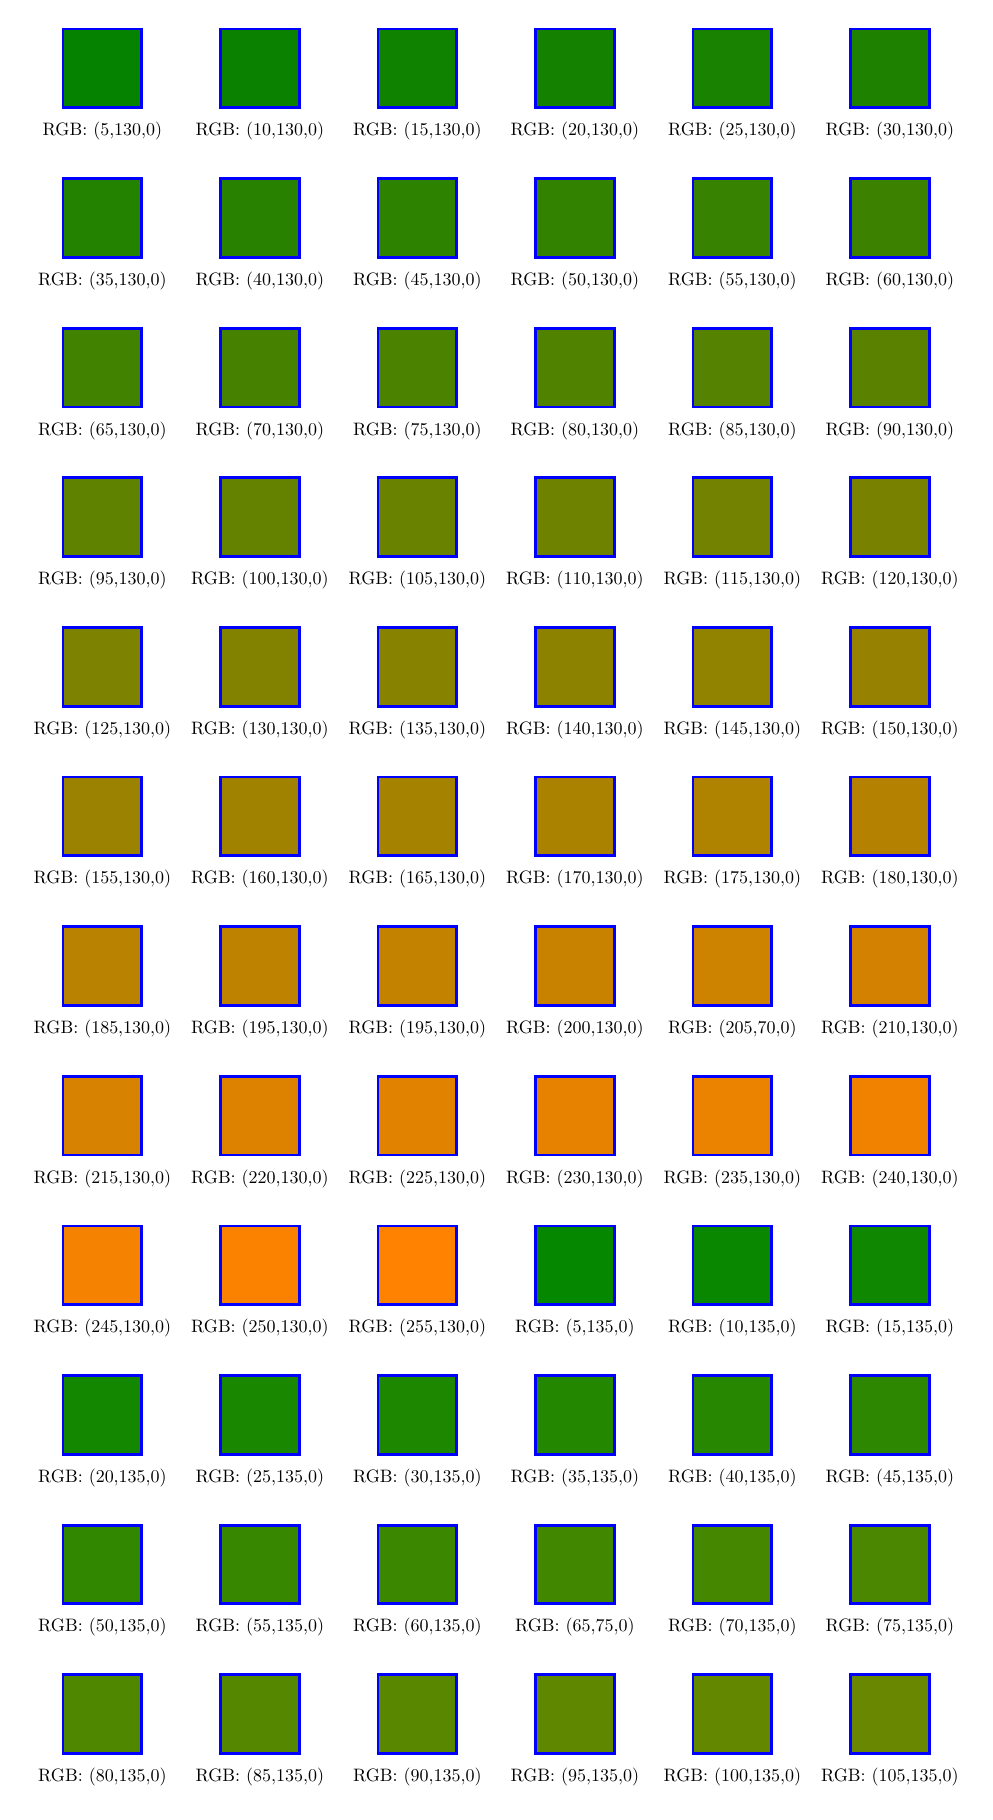
\begin{tikzpicture}

    \filldraw[draw=blue,line width=1,fill=colorR5G130B0]
    (0,0) rectangle (1,1);

    \node[scale=0.65] at (0.5,-0.3) {RGB: (5,130,0)};



    \begin{scope}[xshift=2cm]

      \filldraw[draw=blue,line width=1,fill=colorR10G130B0]
      (0,0) rectangle (1,1);

      \node[scale=0.65] at (0.5,-0.3) {RGB: (10,130,0)};

    \end{scope}



    \begin{scope}[xshift=4cm]

      \filldraw[draw=blue,line width=1,fill=colorR15G130B0]
      (0,0) rectangle (1,1);

      \node[scale=0.65] at (0.5,-0.3) {RGB: (15,130,0)};

    \end{scope}



    \begin{scope}[xshift=6cm]

      \filldraw[draw=blue,line width=1,fill=colorR20G130B0]
      (0,0) rectangle (1,1);

      \node[scale=0.65] at (0.5,-0.3) {RGB: (20,130,0)};

    \end{scope}



    \begin{scope}[xshift=8cm]

      \filldraw[draw=blue,line width=1,fill=colorR25G130B0]
      (0,0) rectangle (1,1);

      \node[scale=0.65] at (0.5,-0.3) {RGB: (25,130,0)};

    \end{scope}



    \begin{scope}[xshift=10cm]

      \filldraw[draw=blue,line width=1,fill=colorR30G130B0]
      (0,0) rectangle (1,1);

      \node[scale=0.65] at (0.5,-0.3) {RGB: (30,130,0)};

    \end{scope}







    \begin{scope}[yshift=-1.9cm]

      \filldraw[draw=blue,line width=1,fill=colorR35G130B0]
      (0,0) rectangle (1,1);

      \node[scale=0.65] at (0.5,-0.3) {RGB: (35,130,0)};

    \end{scope}



    \begin{scope}[xshift=2cm,yshift=-1.9cm]

      \filldraw[draw=blue,line width=1,fill=colorR40G130B0]
      (0,0) rectangle (1,1);

      \node[scale=0.65] at (0.5,-0.3) {RGB: (40,130,0)};

    \end{scope}



    \begin{scope}[xshift=4cm,yshift=-1.9cm]

      \filldraw[draw=blue,line width=1,fill=colorR45G130B0]
      (0,0) rectangle (1,1);

      \node[scale=0.65] at (0.5,-0.3) {RGB: (45,130,0)};

    \end{scope}



    \begin{scope}[xshift=6cm,yshift=-1.9cm]

      \filldraw[draw=blue,line width=1,fill=colorR50G130B0]
      (0,0) rectangle (1,1);

      \node[scale=0.65] at (0.5,-0.3) {RGB: (50,130,0)};

    \end{scope}



    \begin{scope}[xshift=8cm,yshift=-1.9cm]

      \filldraw[draw=blue,line width=1,fill=colorR55G130B0]
      (0,0) rectangle (1,1);

      \node[scale=0.65] at (0.5,-0.3) {RGB: (55,130,0)};

    \end{scope}



    \begin{scope}[xshift=10cm,yshift=-1.9cm]

      \filldraw[draw=blue,line width=1,fill=colorR60G130B0]
      (0,0) rectangle (1,1);

      \node[scale=0.65] at (0.5,-0.3) {RGB: (60,130,0)};

    \end{scope}







    \begin{scope}[yshift=-3.8cm]

      \filldraw[draw=blue,line width=1,fill=colorR65G130B0]
      (0,0) rectangle (1,1);

      \node[scale=0.65] at (0.5,-0.3) {RGB: (65,130,0)};

    \end{scope}



    \begin{scope}[xshift=2cm,yshift=-3.8cm]

      \filldraw[draw=blue,line width=1,fill=colorR70G130B0]
      (0,0) rectangle (1,1);

      \node[scale=0.65] at (0.5,-0.3) {RGB: (70,130,0)};

    \end{scope}



    \begin{scope}[xshift=4cm,yshift=-3.8cm]

      \filldraw[draw=blue,line width=1,fill=colorR75G130B0]
      (0,0) rectangle (1,1);

      \node[scale=0.65] at (0.5,-0.3) {RGB: (75,130,0)};

    \end{scope}



    \begin{scope}[xshift=6cm,yshift=-3.8cm]

      \filldraw[draw=blue,line width=1,fill=colorR80G130B0]
      (0,0) rectangle (1,1);

      \node[scale=0.65] at (0.5,-0.3) {RGB: (80,130,0)};

    \end{scope}



    \begin{scope}[xshift=8cm,yshift=-3.8cm]

      \filldraw[draw=blue,line width=1,fill=colorR85G130B0]
      (0,0) rectangle (1,1);

      \node[scale=0.65] at (0.5,-0.3) {RGB: (85,130,0)};

    \end{scope}



    \begin{scope}[xshift=10cm,yshift=-3.8cm]

      \filldraw[draw=blue,line width=1,fill=colorR90G130B0]
      (0,0) rectangle (1,1);

      \node[scale=0.65] at (0.5,-0.3) {RGB: (90,130,0)};

    \end{scope}







    \begin{scope}[yshift=-5.7cm]

      \filldraw[draw=blue,line width=1,fill=colorR95G130B0]
      (0,0) rectangle (1,1);

      \node[scale=0.65] at (0.5,-0.3) {RGB: (95,130,0)};

    \end{scope}



    \begin{scope}[xshift=2cm,yshift=-5.7cm]

      \filldraw[draw=blue,line width=1,fill=colorR100G130B0]
      (0,0) rectangle (1,1);

      \node[scale=0.65] at (0.5,-0.3) {RGB: (100,130,0)};

    \end{scope}



    \begin{scope}[xshift=4cm,yshift=-5.7cm]

      \filldraw[draw=blue,line width=1,fill=colorR105G130B0]
      (0,0) rectangle (1,1);

      \node[scale=0.65] at (0.5,-0.3) {RGB: (105,130,0)};

    \end{scope}



    \begin{scope}[xshift=6cm,yshift=-5.7cm]

      \filldraw[draw=blue,line width=1,fill=colorR110G130B0]
      (0,0) rectangle (1,1);

      \node[scale=0.65] at (0.5,-0.3) {RGB: (110,130,0)};

    \end{scope}



    \begin{scope}[xshift=8cm,yshift=-5.7cm]

      \filldraw[draw=blue,line width=1,fill=colorR115G130B0]
      (0,0) rectangle (1,1);

      \node[scale=0.65] at (0.5,-0.3) {RGB: (115,130,0)};

    \end{scope}



    \begin{scope}[xshift=10cm,yshift=-5.7cm]

      \filldraw[draw=blue,line width=1,fill=colorR120G130B0]
      (0,0) rectangle (1,1);

      \node[scale=0.65] at (0.5,-0.3) {RGB: (120,130,0)};

    \end{scope}







    \begin{scope}[yshift=-7.6cm]

      \filldraw[draw=blue,line width=1,fill=colorR125G130B0]
      (0,0) rectangle (1,1);

      \node[scale=0.65] at (0.5,-0.3) {RGB: (125,130,0)};

    \end{scope}



    \begin{scope}[xshift=2cm,yshift=-7.6cm]

      \filldraw[draw=blue,line width=1,fill=colorR130G130B0]
      (0,0) rectangle (1,1);

      \node[scale=0.65] at (0.5,-0.3) {RGB: (130,130,0)};

    \end{scope}



    \begin{scope}[xshift=4cm,yshift=-7.6cm]

      \filldraw[draw=blue,line width=1,fill=colorR135G130B0]
      (0,0) rectangle (1,1);

      \node[scale=0.65] at (0.5,-0.3) {RGB: (135,130,0)};

    \end{scope}



    \begin{scope}[xshift=6cm,yshift=-7.6cm]

      \filldraw[draw=blue,line width=1,fill=colorR140G130B0]
      (0,0) rectangle (1,1);

      \node[scale=0.65] at (0.5,-0.3) {RGB: (140,130,0)};

    \end{scope}



    \begin{scope}[xshift=8cm,yshift=-7.6cm]

      \filldraw[draw=blue,line width=1,fill=colorR145G130B0]
      (0,0) rectangle (1,1);

      \node[scale=0.65] at (0.5,-0.3) {RGB: (145,130,0)};

    \end{scope}



    \begin{scope}[xshift=10cm,yshift=-7.6cm]

      \filldraw[draw=blue,line width=1,fill=colorR150G130B0]
      (0,0) rectangle (1,1);

      \node[scale=0.65] at (0.5,-0.3) {RGB: (150,130,0)};

    \end{scope}







    \begin{scope}[yshift=-9.5cm]

      \filldraw[draw=blue,line width=1,fill=colorR155G130B0]
      (0,0) rectangle (1,1);

      \node[scale=0.65] at (0.5,-0.3) {RGB: (155,130,0)};

    \end{scope}



    \begin{scope}[xshift=2cm,yshift=-9.5cm]

      \filldraw[draw=blue,line width=1,fill=colorR160G130B0]
      (0,0) rectangle (1,1);

      \node[scale=0.65] at (0.5,-0.3) {RGB: (160,130,0)};

    \end{scope}



    \begin{scope}[xshift=4cm,yshift=-9.5cm]

      \filldraw[draw=blue,line width=1,fill=colorR165G130B0]
      (0,0) rectangle (1,1);

      \node[scale=0.65] at (0.5,-0.3) {RGB: (165,130,0)};

    \end{scope}



    \begin{scope}[xshift=6cm,yshift=-9.5cm]

      \filldraw[draw=blue,line width=1,fill=colorR170G130B0]
      (0,0) rectangle (1,1);

      \node[scale=0.65] at (0.5,-0.3) {RGB: (170,130,0)};

    \end{scope}



    \begin{scope}[xshift=8cm,yshift=-9.5cm]

      \filldraw[draw=blue,line width=1,fill=colorR175G130B0]
      (0,0) rectangle (1,1);

      \node[scale=0.65] at (0.5,-0.3) {RGB: (175,130,0)};

    \end{scope}



    \begin{scope}[xshift=10cm,yshift=-9.5cm]

      \filldraw[draw=blue,line width=1,fill=colorR180G130B0]
      (0,0) rectangle (1,1);

      \node[scale=0.65] at (0.5,-0.3) {RGB: (180,130,0)};

    \end{scope}







    \begin{scope}[yshift=-11.4cm]

      \filldraw[draw=blue,line width=1,fill=colorR185G130B0]
      (0,0) rectangle (1,1);

      \node[scale=0.65] at (0.5,-0.3) {RGB: (185,130,0)};

    \end{scope}



    \begin{scope}[xshift=2cm,yshift=-11.4cm]

      \filldraw[draw=blue,line width=1,fill=colorR190G130B0]
      (0,0) rectangle (1,1);

      \node[scale=0.65] at (0.5,-0.3) {RGB: (195,130,0)};

    \end{scope}



    \begin{scope}[xshift=4cm,yshift=-11.4cm]

      \filldraw[draw=blue,line width=1,fill=colorR195G130B0]
      (0,0) rectangle (1,1);

      \node[scale=0.65] at (0.5,-0.3) {RGB: (195,130,0)};

    \end{scope}



    \begin{scope}[xshift=6cm,yshift=-11.4cm]

      \filldraw[draw=blue,line width=1,fill=colorR200G130B0]
      (0,0) rectangle (1,1);

      \node[scale=0.65] at (0.5,-0.3) {RGB: (200,130,0)};

    \end{scope}



    \begin{scope}[xshift=8cm,yshift=-11.4cm]

      \filldraw[draw=blue,line width=1,fill=colorR205G130B0]
      (0,0) rectangle (1,1);

      \node[scale=0.65] at (0.5,-0.3) {RGB: (205,70,0)};

    \end{scope}



    \begin{scope}[xshift=10cm,yshift=-11.4cm]

      \filldraw[draw=blue,line width=1,fill=colorR210G130B0]
      (0,0) rectangle (1,1);

      \node[scale=0.65] at (0.5,-0.3) {RGB: (210,130,0)};

    \end{scope}







    \begin{scope}[yshift=-13.3cm]

      \filldraw[draw=blue,line width=1,fill=colorR215G130B0]
      (0,0) rectangle (1,1);

      \node[scale=0.65] at (0.5,-0.3) {RGB: (215,130,0)};

    \end{scope}



    \begin{scope}[xshift=2cm,yshift=-13.3cm]

      \filldraw[draw=blue,line width=1,fill=colorR220G130B0]
      (0,0) rectangle (1,1);

      \node[scale=0.65] at (0.5,-0.3) {RGB: (220,130,0)};

    \end{scope}



    \begin{scope}[xshift=4cm,yshift=-13.3cm]

      \filldraw[draw=blue,line width=1,fill=colorR225G130B0]
      (0,0) rectangle (1,1);

      \node[scale=0.65] at (0.5,-0.3) {RGB: (225,130,0)};

    \end{scope}



    \begin{scope}[xshift=6cm,yshift=-13.3cm]

      \filldraw[draw=blue,line width=1,fill=colorR230G130B0]
      (0,0) rectangle (1,1);

      \node[scale=0.65] at (0.5,-0.3) {RGB: (230,130,0)};

    \end{scope}



    \begin{scope}[xshift=8cm,yshift=-13.3cm]

      \filldraw[draw=blue,line width=1,fill=colorR235G130B0]
      (0,0) rectangle (1,1);

      \node[scale=0.65] at (0.5,-0.3) {RGB: (235,130,0)};

    \end{scope}



    \begin{scope}[xshift=10cm,yshift=-13.3cm]

      \filldraw[draw=blue,line width=1,fill=colorR240G130B0]
      (0,0) rectangle (1,1);

      \node[scale=0.65] at (0.5,-0.3) {RGB: (240,130,0)};

    \end{scope}







    \begin{scope}[yshift=-15.2cm]

      \filldraw[draw=blue,line width=1,fill=colorR245G130B0]
      (0,0) rectangle (1,1);

      \node[scale=0.65] at (0.5,-0.3) {RGB: (245,130,0)};

    \end{scope}



    \begin{scope}[xshift=2cm,yshift=-15.2cm]

      \filldraw[draw=blue,line width=1,fill=colorR250G130B0]
      (0,0) rectangle (1,1);

      \node[scale=0.65] at (0.5,-0.3) {RGB: (250,130,0)};

    \end{scope}



    \begin{scope}[xshift=4cm,yshift=-15.2cm]

      \filldraw[draw=blue,line width=1,fill=colorR255G130B0]
      (0,0) rectangle (1,1);

      \node[scale=0.65] at (0.5,-0.3) {RGB: (255,130,0)};

    \end{scope}



    \begin{scope}[xshift=6cm,yshift=-15.2cm]

      \filldraw[draw=blue,line width=1,fill=colorR5G135B0]
      (0,0) rectangle (1,1);

      \node[scale=0.65] at (0.5,-0.3) {RGB: (5,135,0)};

    \end{scope}



    \begin{scope}[xshift=8cm,yshift=-15.2cm]

      \filldraw[draw=blue,line width=1,fill=colorR10G135B0]
      (0,0) rectangle (1,1);

      \node[scale=0.65] at (0.5,-0.3) {RGB: (10,135,0)};

    \end{scope}



    \begin{scope}[xshift=10cm,yshift=-15.2cm]

      \filldraw[draw=blue,line width=1,fill=colorR15G135B0]
      (0,0) rectangle (1,1);

      \node[scale=0.65] at (0.5,-0.3) {RGB: (15,135,0)};

    \end{scope}







    \begin{scope}[yshift=-17.1cm]

      \filldraw[draw=blue,line width=1,fill=colorR20G135B0]
      (0,0) rectangle (1,1);

      \node[scale=0.65] at (0.5,-0.3) {RGB: (20,135,0)};

    \end{scope}



    \begin{scope}[xshift=2cm,yshift=-17.1cm]

      \filldraw[draw=blue,line width=1,fill=colorR25G135B0]
      (0,0) rectangle (1,1);

      \node[scale=0.65] at (0.5,-0.3) {RGB: (25,135,0)};

    \end{scope}



    \begin{scope}[xshift=4cm,yshift=-17.1cm]

      \filldraw[draw=blue,line width=1,fill=colorR30G135B0]
      (0,0) rectangle (1,1);

      \node[scale=0.65] at (0.5,-0.3) {RGB: (30,135,0)};

    \end{scope}



    \begin{scope}[xshift=6cm,yshift=-17.1cm]

      \filldraw[draw=blue,line width=1,fill=colorR35G135B0]
      (0,0) rectangle (1,1);

      \node[scale=0.65] at (0.5,-0.3) {RGB: (35,135,0)};

    \end{scope}



    \begin{scope}[xshift=8cm,yshift=-17.1cm]

      \filldraw[draw=blue,line width=1,fill=colorR40G135B0]
      (0,0) rectangle (1,1);

      \node[scale=0.65] at (0.5,-0.3) {RGB: (40,135,0)};

    \end{scope}



    \begin{scope}[xshift=10cm,yshift=-17.1cm]

      \filldraw[draw=blue,line width=1,fill=colorR45G135B0]
      (0,0) rectangle (1,1);

      \node[scale=0.65] at (0.5,-0.3) {RGB: (45,135,0)};

    \end{scope}







    \begin{scope}[yshift=-19cm]

      \filldraw[draw=blue,line width=1,fill=colorR50G135B0]
      (0,0) rectangle (1,1);

      \node[scale=0.65] at (0.5,-0.3) {RGB: (50,135,0)};

    \end{scope}



    \begin{scope}[xshift=2cm,yshift=-19cm]

      \filldraw[draw=blue,line width=1,fill=colorR55G135B0]
      (0,0) rectangle (1,1);

      \node[scale=0.65] at (0.5,-0.3) {RGB: (55,135,0)};

    \end{scope}



    \begin{scope}[xshift=4cm,yshift=-19cm]

      \filldraw[draw=blue,line width=1,fill=colorR60G135B0]
      (0,0) rectangle (1,1);

      \node[scale=0.65] at (0.5,-0.3) {RGB: (60,135,0)};

    \end{scope}



    \begin{scope}[xshift=6cm,yshift=-19cm]

      \filldraw[draw=blue,line width=1,fill=colorR65G135B0]
      (0,0) rectangle (1,1);

      \node[scale=0.65] at (0.5,-0.3) {RGB: (65,75,0)};

    \end{scope}



    \begin{scope}[xshift=8cm,yshift=-19cm]

      \filldraw[draw=blue,line width=1,fill=colorR70G135B0]
      (0,0) rectangle (1,1);

      \node[scale=0.65] at (0.5,-0.3) {RGB: (70,135,0)};

    \end{scope}



    \begin{scope}[xshift=10cm,yshift=-19cm]

      \filldraw[draw=blue,line width=1,fill=colorR75G135B0]
      (0,0) rectangle (1,1);

      \node[scale=0.65] at (0.5,-0.3) {RGB: (75,135,0)};

    \end{scope}







    \begin{scope}[yshift=-20.9cm]

      \filldraw[draw=blue,line width=1,fill=colorR80G135B0]
      (0,0) rectangle (1,1);

      \node[scale=0.65] at (0.5,-0.3) {RGB: (80,135,0)};

    \end{scope}



    \begin{scope}[xshift=2cm,yshift=-20.9cm]

      \filldraw[draw=blue,line width=1,fill=colorR85G135B0]
      (0,0) rectangle (1,1);

      \node[scale=0.65] at (0.5,-0.3) {RGB: (85,135,0)};

    \end{scope}



    \begin{scope}[xshift=4cm,yshift=-20.9cm]

      \filldraw[draw=blue,line width=1,fill=colorR90G135B0]
      (0,0) rectangle (1,1);

      \node[scale=0.65] at (0.5,-0.3) {RGB: (90,135,0)};

    \end{scope}



    \begin{scope}[xshift=6cm,yshift=-20.9cm]

      \filldraw[draw=blue,line width=1,fill=colorR95G135B0]
      (0,0) rectangle (1,1);

      \node[scale=0.65] at (0.5,-0.3) {RGB: (95,135,0)};

    \end{scope}



    \begin{scope}[xshift=8cm,yshift=-20.9cm]

      \filldraw[draw=blue,line width=1,fill=colorR100G135B0]
      (0,0) rectangle (1,1);

      \node[scale=0.65] at (0.5,-0.3) {RGB: (100,135,0)};

    \end{scope}



    \begin{scope}[xshift=10cm,yshift=-20.9cm]

      \filldraw[draw=blue,line width=1,fill=colorR105G135B0]
      (0,0) rectangle (1,1);

      \node[scale=0.65] at (0.5,-0.3) {RGB: (105,135,0)};

    \end{scope}

  \end{tikzpicture}

  \caption{Mixed colors in~RGB system: $(5,130,0)$--$(255,130,0)$,
    $(5,135,0)$--$(105,135,0)$}



  \label{fig:Mixed-colors-Part-01}

\end{figure}
% ##################





% ##################
\begin{figure}

  \centering


  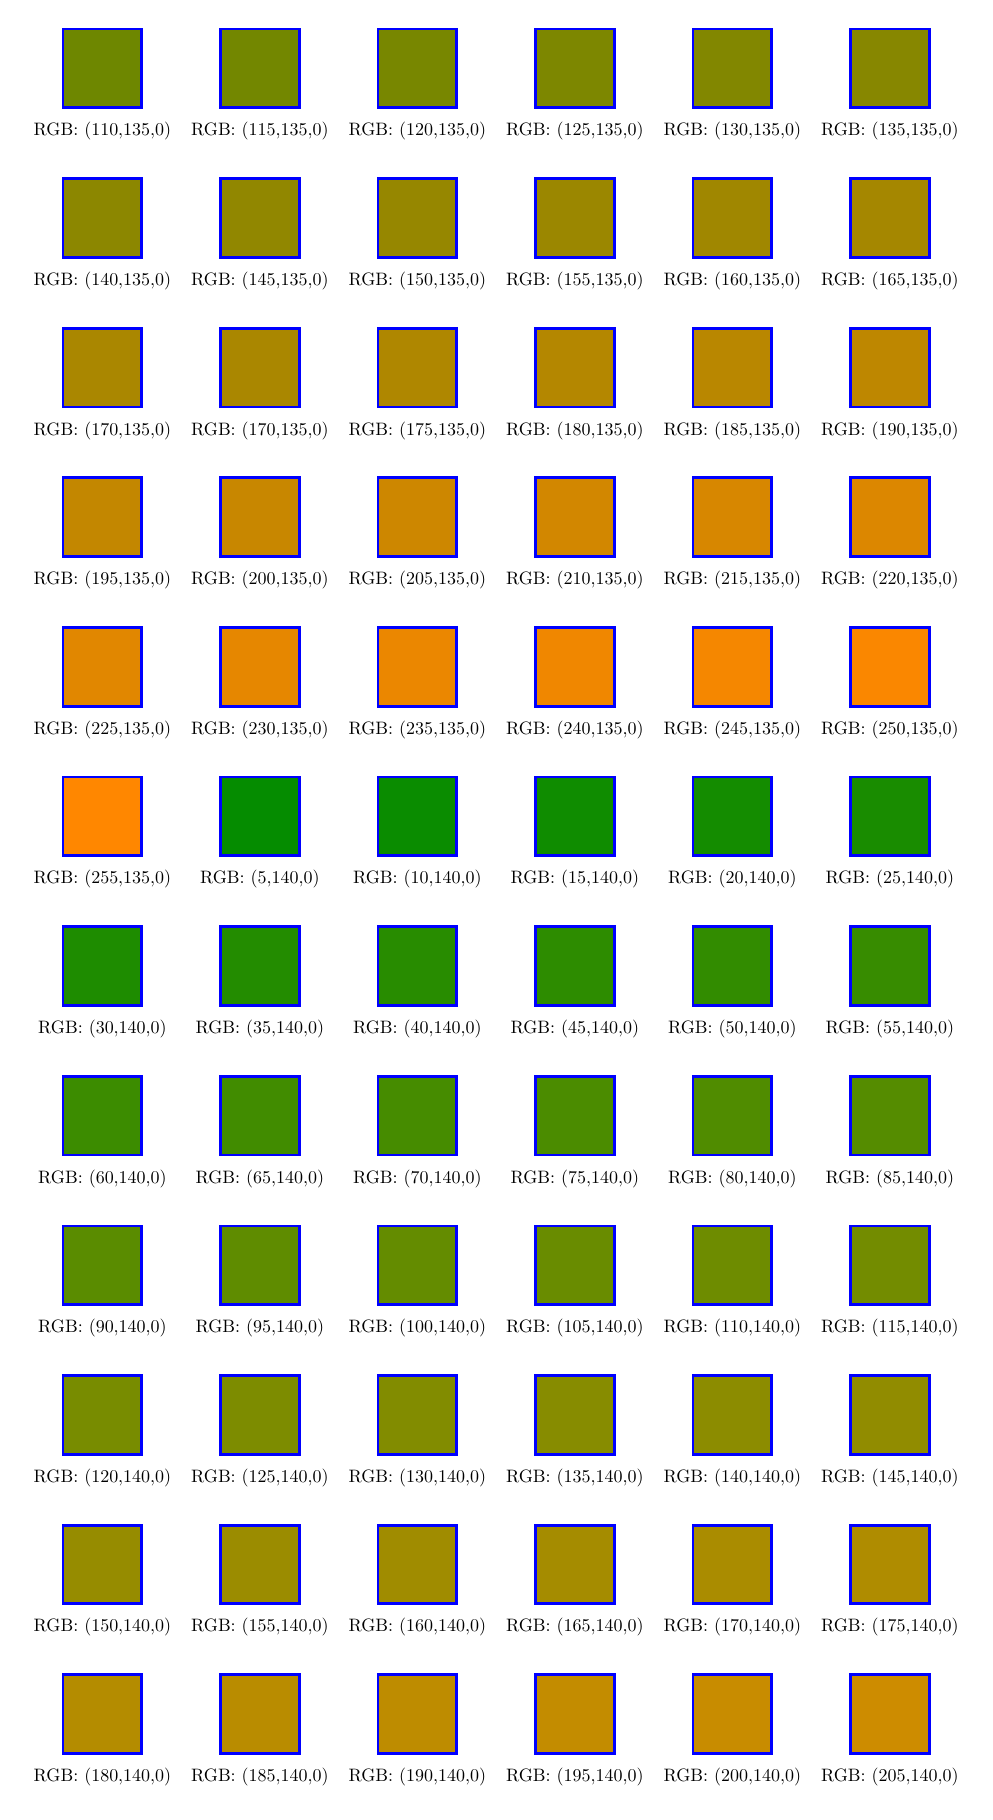
\begin{tikzpicture}

    \filldraw[draw=blue,line width=1,fill=colorR110G135B0]
    (0,0) rectangle (1,1);

    \node[scale=0.65] at (0.5,-0.3) {RGB: (110,135,0)};



    \begin{scope}[xshift=2cm]

      \filldraw[draw=blue,line width=1,fill=colorR115G135B0]
      (0,0) rectangle (1,1);

      \node[scale=0.65] at (0.5,-0.3) {RGB: (115,135,0)};

    \end{scope}



    \begin{scope}[xshift=4cm]

      \filldraw[draw=blue,line width=1,fill=colorR120G135B0]
      (0,0) rectangle (1,1);

      \node[scale=0.65] at (0.5,-0.3) {RGB: (120,135,0)};

    \end{scope}



    \begin{scope}[xshift=6cm]

      \filldraw[draw=blue,line width=1,fill=colorR125G135B0]
      (0,0) rectangle (1,1);

      \node[scale=0.65] at (0.5,-0.3) {RGB: (125,135,0)};

    \end{scope}



    \begin{scope}[xshift=8cm]

      \filldraw[draw=blue,line width=1,fill=colorR130G135B0]
      (0,0) rectangle (1,1);

      \node[scale=0.65] at (0.5,-0.3) {RGB: (130,135,0)};

    \end{scope}



    \begin{scope}[xshift=10cm]

      \filldraw[draw=blue,line width=1,fill=colorR135G135B0]
      (0,0) rectangle (1,1);

      \node[scale=0.65] at (0.5,-0.3) {RGB: (135,135,0)};

    \end{scope}







    \begin{scope}[yshift=-1.9cm]

      \filldraw[draw=blue,line width=1,fill=colorR140G135B0]
      (0,0) rectangle (1,1);

      \node[scale=0.65] at (0.5,-0.3) {RGB: (140,135,0)};

    \end{scope}



    \begin{scope}[xshift=2cm,yshift=-1.9cm]

      \filldraw[draw=blue,line width=1,fill=colorR145G135B0]
      (0,0) rectangle (1,1);

      \node[scale=0.65] at (0.5,-0.3) {RGB: (145,135,0)};

    \end{scope}



    \begin{scope}[xshift=4cm,yshift=-1.9cm]

      \filldraw[draw=blue,line width=1,fill=colorR150G135B0]
      (0,0) rectangle (1,1);

      \node[scale=0.65] at (0.5,-0.3) {RGB: (150,135,0)};

    \end{scope}



    \begin{scope}[xshift=6cm,yshift=-1.9cm]

      \filldraw[draw=blue,line width=1,fill=colorR155G135B0]
      (0,0) rectangle (1,1);

      \node[scale=0.65] at (0.5,-0.3) {RGB: (155,135,0)};

    \end{scope}



    \begin{scope}[xshift=8cm,yshift=-1.9cm]

      \filldraw[draw=blue,line width=1,fill=colorR160G135B0]
      (0,0) rectangle (1,1);

      \node[scale=0.65] at (0.5,-0.3) {RGB: (160,135,0)};

    \end{scope}



    \begin{scope}[xshift=10cm,yshift=-1.9cm]

      \filldraw[draw=blue,line width=1,fill=colorR165G135B0]
      (0,0) rectangle (1,1);

      \node[scale=0.65] at (0.5,-0.3) {RGB: (165,135,0)};

    \end{scope}







    \begin{scope}[yshift=-3.8cm]

      \filldraw[draw=blue,line width=1,fill=colorR170G135B0]
      (0,0) rectangle (1,1);

      \node[scale=0.65] at (0.5,-0.3) {RGB: (170,135,0)};

    \end{scope}



    \begin{scope}[xshift=2cm,yshift=-3.8cm]

      \filldraw[draw=blue,line width=1,fill=colorR170G135B0]
      (0,0) rectangle (1,1);

      \node[scale=0.65] at (0.5,-0.3) {RGB: (170,135,0)};

    \end{scope}



    \begin{scope}[xshift=4cm,yshift=-3.8cm]

      \filldraw[draw=blue,line width=1,fill=colorR175G135B0]
      (0,0) rectangle (1,1);

      \node[scale=0.65] at (0.5,-0.3) {RGB: (175,135,0)};

    \end{scope}



    \begin{scope}[xshift=6cm,yshift=-3.8cm]

      \filldraw[draw=blue,line width=1,fill=colorR180G135B0]
      (0,0) rectangle (1,1);

      \node[scale=0.65] at (0.5,-0.3) {RGB: (180,135,0)};

    \end{scope}



    \begin{scope}[xshift=8cm,yshift=-3.8cm]

      \filldraw[draw=blue,line width=1,fill=colorR185G135B0]
      (0,0) rectangle (1,1);

      \node[scale=0.65] at (0.5,-0.3) {RGB: (185,135,0)};

    \end{scope}



    \begin{scope}[xshift=10cm,yshift=-3.8cm]

      \filldraw[draw=blue,line width=1,fill=colorR190G135B0]
      (0,0) rectangle (1,1);

      \node[scale=0.65] at (0.5,-0.3) {RGB: (190,135,0)};

    \end{scope}







    \begin{scope}[yshift=-5.7cm]

      \filldraw[draw=blue,line width=1,fill=colorR195G135B0]
      (0,0) rectangle (1,1);

      \node[scale=0.65] at (0.5,-0.3) {RGB: (195,135,0)};

    \end{scope}



    \begin{scope}[xshift=2cm,yshift=-5.7cm]

      \filldraw[draw=blue,line width=1,fill=colorR200G135B0]
      (0,0) rectangle (1,1);

      \node[scale=0.65] at (0.5,-0.3) {RGB: (200,135,0)};

    \end{scope}



    \begin{scope}[xshift=4cm,yshift=-5.7cm]

      \filldraw[draw=blue,line width=1,fill=colorR205G135B0]
      (0,0) rectangle (1,1);

      \node[scale=0.65] at (0.5,-0.3) {RGB: (205,135,0)};

    \end{scope}



    \begin{scope}[xshift=6cm,yshift=-5.7cm]

      \filldraw[draw=blue,line width=1,fill=colorR210G135B0]
      (0,0) rectangle (1,1);

      \node[scale=0.65] at (0.5,-0.3) {RGB: (210,135,0)};

    \end{scope}



    \begin{scope}[xshift=8cm,yshift=-5.7cm]

      \filldraw[draw=blue,line width=1,fill=colorR215G135B0]
      (0,0) rectangle (1,1);

      \node[scale=0.65] at (0.5,-0.3) {RGB: (215,135,0)};

    \end{scope}



    \begin{scope}[xshift=10cm,yshift=-5.7cm]

      \filldraw[draw=blue,line width=1,fill=colorR220G135B0]
      (0,0) rectangle (1,1);

      \node[scale=0.65] at (0.5,-0.3) {RGB: (220,135,0)};

    \end{scope}







    \begin{scope}[yshift=-7.6cm]

      \filldraw[draw=blue,line width=1,fill=colorR225G135B0]
      (0,0) rectangle (1,1);

      \node[scale=0.65] at (0.5,-0.3) {RGB: (225,135,0)};

    \end{scope}



    \begin{scope}[xshift=2cm,yshift=-7.6cm]

      \filldraw[draw=blue,line width=1,fill=colorR230G135B0]
      (0,0) rectangle (1,1);

      \node[scale=0.65] at (0.5,-0.3) {RGB: (230,135,0)};

    \end{scope}



    \begin{scope}[xshift=4cm,yshift=-7.6cm]

      \filldraw[draw=blue,line width=1,fill=colorR235G135B0]
      (0,0) rectangle (1,1);

      \node[scale=0.65] at (0.5,-0.3) {RGB: (235,135,0)};

    \end{scope}



    \begin{scope}[xshift=6cm,yshift=-7.6cm]

      \filldraw[draw=blue,line width=1,fill=colorR240G135B0]
      (0,0) rectangle (1,1);

      \node[scale=0.65] at (0.5,-0.3) {RGB: (240,135,0)};

    \end{scope}



    \begin{scope}[xshift=8cm,yshift=-7.6cm]

      \filldraw[draw=blue,line width=1,fill=colorR245G135B0]
      (0,0) rectangle (1,1);

      \node[scale=0.65] at (0.5,-0.3) {RGB: (245,135,0)};

    \end{scope}



    \begin{scope}[xshift=10cm,yshift=-7.6cm]

      \filldraw[draw=blue,line width=1,fill=colorR250G135B0]
      (0,0) rectangle (1,1);

      \node[scale=0.65] at (0.5,-0.3) {RGB: (250,135,0)};

    \end{scope}







    \begin{scope}[yshift=-9.5cm]

      \filldraw[draw=blue,line width=1,fill=colorR255G135B0]
      (0,0) rectangle (1,1);

      \node[scale=0.65] at (0.5,-0.3) {RGB: (255,135,0)};

    \end{scope}



    \begin{scope}[xshift=2cm,yshift=-9.5cm]

      \filldraw[draw=blue,line width=1,fill=colorR5G140B0]
      (0,0) rectangle (1,1);

      \node[scale=0.65] at (0.5,-0.3) {RGB: (5,140,0)};

    \end{scope}



    \begin{scope}[xshift=4cm,yshift=-9.5cm]

      \filldraw[draw=blue,line width=1,fill=colorR10G140B0]
      (0,0) rectangle (1,1);

      \node[scale=0.65] at (0.5,-0.3) {RGB: (10,140,0)};

    \end{scope}



    \begin{scope}[xshift=6cm,yshift=-9.5cm]

      \filldraw[draw=blue,line width=1,fill=colorR15G140B0]
      (0,0) rectangle (1,1);

      \node[scale=0.65] at (0.5,-0.3) {RGB: (15,140,0)};

    \end{scope}



    \begin{scope}[xshift=8cm,yshift=-9.5cm]

      \filldraw[draw=blue,line width=1,fill=colorR20G140B0]
      (0,0) rectangle (1,1);

      \node[scale=0.65] at (0.5,-0.3) {RGB: (20,140,0)};

    \end{scope}



    \begin{scope}[xshift=10cm,yshift=-9.5cm]

      \filldraw[draw=blue,line width=1,fill=colorR25G140B0]
      (0,0) rectangle (1,1);

      \node[scale=0.65] at (0.5,-0.3) {RGB: (25,140,0)};

    \end{scope}







    \begin{scope}[yshift=-11.4cm]

      \filldraw[draw=blue,line width=1,fill=colorR30G140B0]
      (0,0) rectangle (1,1);

      \node[scale=0.65] at (0.5,-0.3) {RGB: (30,140,0)};

    \end{scope}



    \begin{scope}[xshift=2cm,yshift=-11.4cm]

      \filldraw[draw=blue,line width=1,fill=colorR35G140B0]
      (0,0) rectangle (1,1);

      \node[scale=0.65] at (0.5,-0.3) {RGB: (35,140,0)};

    \end{scope}



    \begin{scope}[xshift=4cm,yshift=-11.4cm]

      \filldraw[draw=blue,line width=1,fill=colorR40G140B0]
      (0,0) rectangle (1,1);

      \node[scale=0.65] at (0.5,-0.3) {RGB: (40,140,0)};

    \end{scope}



    \begin{scope}[xshift=6cm,yshift=-11.4cm]

      \filldraw[draw=blue,line width=1,fill=colorR45G140B0]
      (0,0) rectangle (1,1);

      \node[scale=0.65] at (0.5,-0.3) {RGB: (45,140,0)};

    \end{scope}



    \begin{scope}[xshift=8cm,yshift=-11.4cm]

      \filldraw[draw=blue,line width=1,fill=colorR50G140B0]
      (0,0) rectangle (1,1);

      \node[scale=0.65] at (0.5,-0.3) {RGB: (50,140,0)};

    \end{scope}



    \begin{scope}[xshift=10cm,yshift=-11.4cm]

      \filldraw[draw=blue,line width=1,fill=colorR55G140B0]
      (0,0) rectangle (1,1);

      \node[scale=0.65] at (0.5,-0.3) {RGB: (55,140,0)};

    \end{scope}







    \begin{scope}[yshift=-13.3cm]

      \filldraw[draw=blue,line width=1,fill=colorR60G140B0]
      (0,0) rectangle (1,1);

      \node[scale=0.65] at (0.5,-0.3) {RGB: (60,140,0)};

    \end{scope}



    \begin{scope}[xshift=2cm,yshift=-13.3cm]

      \filldraw[draw=blue,line width=1,fill=colorR65G140B0]
      (0,0) rectangle (1,1);

      \node[scale=0.65] at (0.5,-0.3) {RGB: (65,140,0)};

    \end{scope}



    \begin{scope}[xshift=4cm,yshift=-13.3cm]

      \filldraw[draw=blue,line width=1,fill=colorR70G140B0]
      (0,0) rectangle (1,1);

      \node[scale=0.65] at (0.5,-0.3) {RGB: (70,140,0)};

    \end{scope}



    \begin{scope}[xshift=6cm,yshift=-13.3cm]

      \filldraw[draw=blue,line width=1,fill=colorR75G140B0]
      (0,0) rectangle (1,1);

      \node[scale=0.65] at (0.5,-0.3) {RGB: (75,140,0)};

    \end{scope}



    \begin{scope}[xshift=8cm,yshift=-13.3cm]

      \filldraw[draw=blue,line width=1,fill=colorR80G140B0]
      (0,0) rectangle (1,1);

      \node[scale=0.65] at (0.5,-0.3) {RGB: (80,140,0)};

    \end{scope}



    \begin{scope}[xshift=10cm,yshift=-13.3cm]

      \filldraw[draw=blue,line width=1,fill=colorR85G140B0]
      (0,0) rectangle (1,1);

      \node[scale=0.65] at (0.5,-0.3) {RGB: (85,140,0)};

    \end{scope}







    \begin{scope}[yshift=-15.2cm]

      \filldraw[draw=blue,line width=1,fill=colorR90G140B0]
      (0,0) rectangle (1,1);

      \node[scale=0.65] at (0.5,-0.3) {RGB: (90,140,0)};

    \end{scope}



    \begin{scope}[xshift=2cm,yshift=-15.2cm]

      \filldraw[draw=blue,line width=1,fill=colorR95G140B0]
      (0,0) rectangle (1,1);

      \node[scale=0.65] at (0.5,-0.3) {RGB: (95,140,0)};

    \end{scope}



    \begin{scope}[xshift=4cm,yshift=-15.2cm]

      \filldraw[draw=blue,line width=1,fill=colorR100G140B0]
      (0,0) rectangle (1,1);

      \node[scale=0.65] at (0.5,-0.3) {RGB: (100,140,0)};

    \end{scope}



    \begin{scope}[xshift=6cm,yshift=-15.2cm]

      \filldraw[draw=blue,line width=1,fill=colorR105G140B0]
      (0,0) rectangle (1,1);

      \node[scale=0.65] at (0.5,-0.3) {RGB: (105,140,0)};

    \end{scope}



    \begin{scope}[xshift=8cm,yshift=-15.2cm]

      \filldraw[draw=blue,line width=1,fill=colorR110G140B0]
      (0,0) rectangle (1,1);

      \node[scale=0.65] at (0.5,-0.3) {RGB: (110,140,0)};

    \end{scope}



    \begin{scope}[xshift=10cm,yshift=-15.2cm]

      \filldraw[draw=blue,line width=1,fill=colorR115G140B0]
      (0,0) rectangle (1,1);

      \node[scale=0.65] at (0.5,-0.3) {RGB: (115,140,0)};

    \end{scope}







    \begin{scope}[yshift=-17.1cm]

      \filldraw[draw=blue,line width=1,fill=colorR120G140B0]
      (0,0) rectangle (1,1);

      \node[scale=0.65] at (0.5,-0.3) {RGB: (120,140,0)};

    \end{scope}



    \begin{scope}[xshift=2cm,yshift=-17.1cm]

      \filldraw[draw=blue,line width=1,fill=colorR125G140B0]
      (0,0) rectangle (1,1);

      \node[scale=0.65] at (0.5,-0.3) {RGB: (125,140,0)};

    \end{scope}



    \begin{scope}[xshift=4cm,yshift=-17.1cm]

      \filldraw[draw=blue,line width=1,fill=colorR130G140B0]
      (0,0) rectangle (1,1);

      \node[scale=0.65] at (0.5,-0.3) {RGB: (130,140,0)};

    \end{scope}



    \begin{scope}[xshift=6cm,yshift=-17.1cm]

      \filldraw[draw=blue,line width=1,fill=colorR135G140B0]
      (0,0) rectangle (1,1);

      \node[scale=0.65] at (0.5,-0.3) {RGB: (135,140,0)};

    \end{scope}



    \begin{scope}[xshift=8cm,yshift=-17.1cm]

      \filldraw[draw=blue,line width=1,fill=colorR140G140B0]
      (0,0) rectangle (1,1);

      \node[scale=0.65] at (0.5,-0.3) {RGB: (140,140,0)};

    \end{scope}



    \begin{scope}[xshift=10cm,yshift=-17.1cm]

      \filldraw[draw=blue,line width=1,fill=colorR145G140B0]
      (0,0) rectangle (1,1);

      \node[scale=0.65] at (0.5,-0.3) {RGB: (145,140,0)};

    \end{scope}







    \begin{scope}[yshift=-19cm]

      \filldraw[draw=blue,line width=1,fill=colorR150G140B0]
      (0,0) rectangle (1,1);

      \node[scale=0.65] at (0.5,-0.3) {RGB: (150,140,0)};

    \end{scope}



    \begin{scope}[xshift=2cm,yshift=-19cm]

      \filldraw[draw=blue,line width=1,fill=colorR155G140B0]
      (0,0) rectangle (1,1);

      \node[scale=0.65] at (0.5,-0.3) {RGB: (155,140,0)};

    \end{scope}



    \begin{scope}[xshift=4cm,yshift=-19cm]

      \filldraw[draw=blue,line width=1,fill=colorR160G140B0]
      (0,0) rectangle (1,1);

      \node[scale=0.65] at (0.5,-0.3) {RGB: (160,140,0)};

    \end{scope}



    \begin{scope}[xshift=6cm,yshift=-19cm]

      \filldraw[draw=blue,line width=1,fill=colorR165G140B0]
      (0,0) rectangle (1,1);

      \node[scale=0.65] at (0.5,-0.3) {RGB: (165,140,0)};

    \end{scope}



    \begin{scope}[xshift=8cm,yshift=-19cm]

      \filldraw[draw=blue,line width=1,fill=colorR170G140B0]
      (0,0) rectangle (1,1);

      \node[scale=0.65] at (0.5,-0.3) {RGB: (170,140,0)};

    \end{scope}



    \begin{scope}[xshift=10cm,yshift=-19cm]

      \filldraw[draw=blue,line width=1,fill=colorR175G140B0]
      (0,0) rectangle (1,1);

      \node[scale=0.65] at (0.5,-0.3) {RGB: (175,140,0)};

    \end{scope}







    \begin{scope}[yshift=-20.9cm]

      \filldraw[draw=blue,line width=1,fill=colorR180G140B0]
      (0,0) rectangle (1,1);

      \node[scale=0.65] at (0.5,-0.3) {RGB: (180,140,0)};

    \end{scope}



    \begin{scope}[xshift=2cm,yshift=-20.9cm]

      \filldraw[draw=blue,line width=1,fill=colorR185G140B0]
      (0,0) rectangle (1,1);

      \node[scale=0.65] at (0.5,-0.3) {RGB: (185,140,0)};

    \end{scope}



    \begin{scope}[xshift=4cm,yshift=-20.9cm]

      \filldraw[draw=blue,line width=1,fill=colorR190G140B0]
      (0,0) rectangle (1,1);

      \node[scale=0.65] at (0.5,-0.3) {RGB: (190,140,0)};

    \end{scope}



    \begin{scope}[xshift=6cm,yshift=-20.9cm]

      \filldraw[draw=blue,line width=1,fill=colorR195G140B0]
      (0,0) rectangle (1,1);

      \node[scale=0.65] at (0.5,-0.3) {RGB: (195,140,0)};

    \end{scope}



    \begin{scope}[xshift=8cm,yshift=-20.9cm]

      \filldraw[draw=blue,line width=1,fill=colorR200G140B0]
      (0,0) rectangle (1,1);

      \node[scale=0.65] at (0.5,-0.3) {RGB: (200,140,0)};

    \end{scope}



    \begin{scope}[xshift=10cm,yshift=-20.9cm]

      \filldraw[draw=blue,line width=1,fill=colorR205G140B0]
      (0,0) rectangle (1,1);

      \node[scale=0.65] at (0.5,-0.3) {RGB: (205,140,0)};

    \end{scope}

  \end{tikzpicture}

  \caption{Mixed colors in~RGB system: $(110,135,0)$--$(255,135,0)$,
    $(5,140,0)$--$(205,140,0)$}



  \label{fig:Mixed-colors-Part-02}

\end{figure}
% ##################





% ##################
\begin{figure}

  \centering


  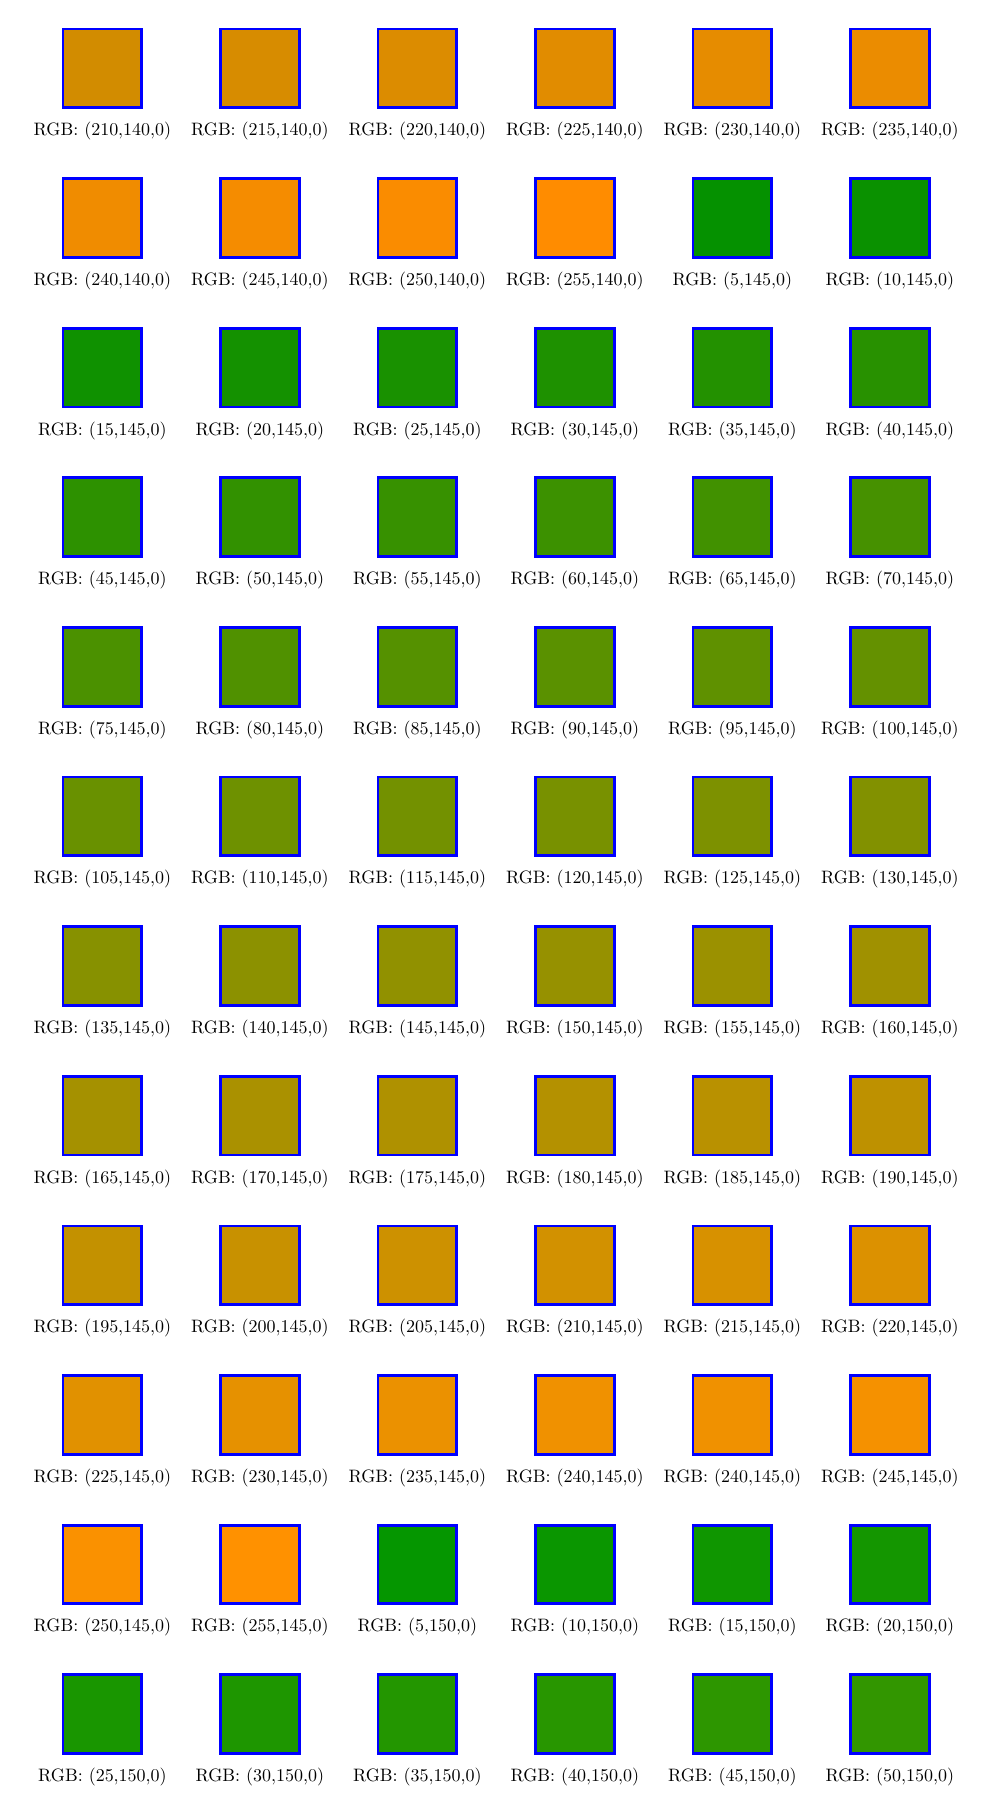
\begin{tikzpicture}

    \filldraw[draw=blue,line width=1,fill=colorR210G140B0]
    (0,0) rectangle (1,1);

    \node[scale=0.65] at (0.5,-0.3) {RGB: (210,140,0)};



    \begin{scope}[xshift=2cm]

      \filldraw[draw=blue,line width=1,fill=colorR215G140B0]
      (0,0) rectangle (1,1);

      \node[scale=0.65] at (0.5,-0.3) {RGB: (215,140,0)};

    \end{scope}



    \begin{scope}[xshift=4cm]

      \filldraw[draw=blue,line width=1,fill=colorR220G140B0]
      (0,0) rectangle (1,1);

      \node[scale=0.65] at (0.5,-0.3) {RGB: (220,140,0)};

    \end{scope}



    \begin{scope}[xshift=6cm]

      \filldraw[draw=blue,line width=1,fill=colorR225G140B0]
      (0,0) rectangle (1,1);

      \node[scale=0.65] at (0.5,-0.3) {RGB: (225,140,0)};

    \end{scope}



    \begin{scope}[xshift=8cm]

      \filldraw[draw=blue,line width=1,fill=colorR230G140B0]
      (0,0) rectangle (1,1);

      \node[scale=0.65] at (0.5,-0.3) {RGB: (230,140,0)};

    \end{scope}



    \begin{scope}[xshift=10cm]

      \filldraw[draw=blue,line width=1,fill=colorR235G140B0]
      (0,0) rectangle (1,1);

      \node[scale=0.65] at (0.5,-0.3) {RGB: (235,140,0)};

    \end{scope}







    \begin{scope}[yshift=-1.9cm]

      \filldraw[draw=blue,line width=1,fill=colorR240G140B0]
      (0,0) rectangle (1,1);

      \node[scale=0.65] at (0.5,-0.3) {RGB: (240,140,0)};

    \end{scope}



    \begin{scope}[xshift=2cm,yshift=-1.9cm]

      \filldraw[draw=blue,line width=1,fill=colorR245G140B0]
      (0,0) rectangle (1,1);

      \node[scale=0.65] at (0.5,-0.3) {RGB: (245,140,0)};

    \end{scope}



    \begin{scope}[xshift=4cm,yshift=-1.9cm]

      \filldraw[draw=blue,line width=1,fill=colorR250G140B0]
      (0,0) rectangle (1,1);

      \node[scale=0.65] at (0.5,-0.3) {RGB: (250,140,0)};

    \end{scope}



    \begin{scope}[xshift=6cm,yshift=-1.9cm]

      \filldraw[draw=blue,line width=1,fill=colorR255G140B0]
      (0,0) rectangle (1,1);

      \node[scale=0.65] at (0.5,-0.3) {RGB: (255,140,0)};

    \end{scope}



    \begin{scope}[xshift=8cm,yshift=-1.9cm]

      \filldraw[draw=blue,line width=1,fill=colorR5G145B0]
      (0,0) rectangle (1,1);

      \node[scale=0.65] at (0.5,-0.3) {RGB: (5,145,0)};

    \end{scope}



    \begin{scope}[xshift=10cm,yshift=-1.9cm]

      \filldraw[draw=blue,line width=1,fill=colorR10G145B0]
      (0,0) rectangle (1,1);

      \node[scale=0.65] at (0.5,-0.3) {RGB: (10,145,0)};

    \end{scope}







    \begin{scope}[yshift=-3.8cm]

      \filldraw[draw=blue,line width=1,fill=colorR15G145B0]
      (0,0) rectangle (1,1);

      \node[scale=0.65] at (0.5,-0.3) {RGB: (15,145,0)};

    \end{scope}



    \begin{scope}[xshift=2cm,yshift=-3.8cm]

      \filldraw[draw=blue,line width=1,fill=colorR20G145B0]
      (0,0) rectangle (1,1);

      \node[scale=0.65] at (0.5,-0.3) {RGB: (20,145,0)};

    \end{scope}



    \begin{scope}[xshift=4cm,yshift=-3.8cm]

      \filldraw[draw=blue,line width=1,fill=colorR25G145B0]
      (0,0) rectangle (1,1);

      \node[scale=0.65] at (0.5,-0.3) {RGB: (25,145,0)};

    \end{scope}



    \begin{scope}[xshift=6cm,yshift=-3.8cm]

      \filldraw[draw=blue,line width=1,fill=colorR30G145B0]
      (0,0) rectangle (1,1);

      \node[scale=0.65] at (0.5,-0.3) {RGB: (30,145,0)};

    \end{scope}



    \begin{scope}[xshift=8cm,yshift=-3.8cm]

      \filldraw[draw=blue,line width=1,fill=colorR35G145B0]
      (0,0) rectangle (1,1);

      \node[scale=0.65] at (0.5,-0.3) {RGB: (35,145,0)};

    \end{scope}



    \begin{scope}[xshift=10cm,yshift=-3.8cm]

      \filldraw[draw=blue,line width=1,fill=colorR40G145B0]
      (0,0) rectangle (1,1);

      \node[scale=0.65] at (0.5,-0.3) {RGB: (40,145,0)};

    \end{scope}







    \begin{scope}[yshift=-5.7cm]

      \filldraw[draw=blue,line width=1,fill=colorR45G145B0]
      (0,0) rectangle (1,1);

      \node[scale=0.65] at (0.5,-0.3) {RGB: (45,145,0)};

    \end{scope}



    \begin{scope}[xshift=2cm,yshift=-5.7cm]

      \filldraw[draw=blue,line width=1,fill=colorR50G145B0]
      (0,0) rectangle (1,1);

      \node[scale=0.65] at (0.5,-0.3) {RGB: (50,145,0)};

    \end{scope}



    \begin{scope}[xshift=4cm,yshift=-5.7cm]

      \filldraw[draw=blue,line width=1,fill=colorR55G145B0]
      (0,0) rectangle (1,1);

      \node[scale=0.65] at (0.5,-0.3) {RGB: (55,145,0)};

    \end{scope}



    \begin{scope}[xshift=6cm,yshift=-5.7cm]

      \filldraw[draw=blue,line width=1,fill=colorR60G145B0]
      (0,0) rectangle (1,1);

      \node[scale=0.65] at (0.5,-0.3) {RGB: (60,145,0)};

    \end{scope}



    \begin{scope}[xshift=8cm,yshift=-5.7cm]

      \filldraw[draw=blue,line width=1,fill=colorR65G145B0]
      (0,0) rectangle (1,1);

      \node[scale=0.65] at (0.5,-0.3) {RGB: (65,145,0)};

    \end{scope}



    \begin{scope}[xshift=10cm,yshift=-5.7cm]

      \filldraw[draw=blue,line width=1,fill=colorR70G145B0]
      (0,0) rectangle (1,1);

      \node[scale=0.65] at (0.5,-0.3) {RGB: (70,145,0)};

    \end{scope}







    \begin{scope}[yshift=-7.6cm]

      \filldraw[draw=blue,line width=1,fill=colorR75G145B0]
      (0,0) rectangle (1,1);

      \node[scale=0.65] at (0.5,-0.3) {RGB: (75,145,0)};

    \end{scope}



    \begin{scope}[xshift=2cm,yshift=-7.6cm]

      \filldraw[draw=blue,line width=1,fill=colorR80G145B0]
      (0,0) rectangle (1,1);

      \node[scale=0.65] at (0.5,-0.3) {RGB: (80,145,0)};

    \end{scope}



    \begin{scope}[xshift=4cm,yshift=-7.6cm]

      \filldraw[draw=blue,line width=1,fill=colorR85G145B0]
      (0,0) rectangle (1,1);

      \node[scale=0.65] at (0.5,-0.3) {RGB: (85,145,0)};

    \end{scope}



    \begin{scope}[xshift=6cm,yshift=-7.6cm]

      \filldraw[draw=blue,line width=1,fill=colorR90G145B0]
      (0,0) rectangle (1,1);

      \node[scale=0.65] at (0.5,-0.3) {RGB: (90,145,0)};

    \end{scope}



    \begin{scope}[xshift=8cm,yshift=-7.6cm]

      \filldraw[draw=blue,line width=1,fill=colorR95G145B0]
      (0,0) rectangle (1,1);

      \node[scale=0.65] at (0.5,-0.3) {RGB: (95,145,0)};

    \end{scope}



    \begin{scope}[xshift=10cm,yshift=-7.6cm]

      \filldraw[draw=blue,line width=1,fill=colorR100G145B0]
      (0,0) rectangle (1,1);

      \node[scale=0.65] at (0.5,-0.3) {RGB: (100,145,0)};

    \end{scope}







    \begin{scope}[yshift=-9.5cm]

      \filldraw[draw=blue,line width=1,fill=colorR105G145B0]
      (0,0) rectangle (1,1);

      \node[scale=0.65] at (0.5,-0.3) {RGB: (105,145,0)};

    \end{scope}



    \begin{scope}[xshift=2cm,yshift=-9.5cm]

      \filldraw[draw=blue,line width=1,fill=colorR110G145B0]
      (0,0) rectangle (1,1);

      \node[scale=0.65] at (0.5,-0.3) {RGB: (110,145,0)};

    \end{scope}



    \begin{scope}[xshift=4cm,yshift=-9.5cm]

      \filldraw[draw=blue,line width=1,fill=colorR115G145B0]
      (0,0) rectangle (1,1);

      \node[scale=0.65] at (0.5,-0.3) {RGB: (115,145,0)};

    \end{scope}



    \begin{scope}[xshift=6cm,yshift=-9.5cm]

      \filldraw[draw=blue,line width=1,fill=colorR120G145B0]
      (0,0) rectangle (1,1);

      \node[scale=0.65] at (0.5,-0.3) {RGB: (120,145,0)};

    \end{scope}



    \begin{scope}[xshift=8cm,yshift=-9.5cm]

      \filldraw[draw=blue,line width=1,fill=colorR125G145B0]
      (0,0) rectangle (1,1);

      \node[scale=0.65] at (0.5,-0.3) {RGB: (125,145,0)};

    \end{scope}



    \begin{scope}[xshift=10cm,yshift=-9.5cm]

      \filldraw[draw=blue,line width=1,fill=colorR130G145B0]
      (0,0) rectangle (1,1);

      \node[scale=0.65] at (0.5,-0.3) {RGB: (130,145,0)};

    \end{scope}







    \begin{scope}[yshift=-11.4cm]

      \filldraw[draw=blue,line width=1,fill=colorR135G145B0]
      (0,0) rectangle (1,1);

      \node[scale=0.65] at (0.5,-0.3) {RGB: (135,145,0)};

    \end{scope}



    \begin{scope}[xshift=2cm,yshift=-11.4cm]

      \filldraw[draw=blue,line width=1,fill=colorR140G145B0]
      (0,0) rectangle (1,1);

      \node[scale=0.65] at (0.5,-0.3) {RGB: (140,145,0)};

    \end{scope}



    \begin{scope}[xshift=4cm,yshift=-11.4cm]

      \filldraw[draw=blue,line width=1,fill=colorR145G145B0]
      (0,0) rectangle (1,1);

      \node[scale=0.65] at (0.5,-0.3) {RGB: (145,145,0)};

    \end{scope}



    \begin{scope}[xshift=6cm,yshift=-11.4cm]

      \filldraw[draw=blue,line width=1,fill=colorR150G145B0]
      (0,0) rectangle (1,1);

      \node[scale=0.65] at (0.5,-0.3) {RGB: (150,145,0)};

    \end{scope}



    \begin{scope}[xshift=8cm,yshift=-11.4cm]

      \filldraw[draw=blue,line width=1,fill=colorR155G145B0]
      (0,0) rectangle (1,1);

      \node[scale=0.65] at (0.5,-0.3) {RGB: (155,145,0)};

    \end{scope}



    \begin{scope}[xshift=10cm,yshift=-11.4cm]

      \filldraw[draw=blue,line width=1,fill=colorR160G145B0]
      (0,0) rectangle (1,1);

      \node[scale=0.65] at (0.5,-0.3) {RGB: (160,145,0)};

    \end{scope}







    \begin{scope}[yshift=-13.3cm]

      \filldraw[draw=blue,line width=1,fill=colorR165G145B0]
      (0,0) rectangle (1,1);

      \node[scale=0.65] at (0.5,-0.3) {RGB: (165,145,0)};

    \end{scope}



    \begin{scope}[xshift=2cm,yshift=-13.3cm]

      \filldraw[draw=blue,line width=1,fill=colorR170G145B0]
      (0,0) rectangle (1,1);

      \node[scale=0.65] at (0.5,-0.3) {RGB: (170,145,0)};

    \end{scope}



    \begin{scope}[xshift=4cm,yshift=-13.3cm]

      \filldraw[draw=blue,line width=1,fill=colorR175G145B0]
      (0,0) rectangle (1,1);

      \node[scale=0.65] at (0.5,-0.3) {RGB: (175,145,0)};

    \end{scope}



    \begin{scope}[xshift=6cm,yshift=-13.3cm]

      \filldraw[draw=blue,line width=1,fill=colorR180G145B0]
      (0,0) rectangle (1,1);

      \node[scale=0.65] at (0.5,-0.3) {RGB: (180,145,0)};

    \end{scope}



    \begin{scope}[xshift=8cm,yshift=-13.3cm]

      \filldraw[draw=blue,line width=1,fill=colorR185G145B0]
      (0,0) rectangle (1,1);

      \node[scale=0.65] at (0.5,-0.3) {RGB: (185,145,0)};

    \end{scope}



    \begin{scope}[xshift=10cm,yshift=-13.3cm]

      \filldraw[draw=blue,line width=1,fill=colorR190G145B0]
      (0,0) rectangle (1,1);

      \node[scale=0.65] at (0.5,-0.3) {RGB: (190,145,0)};

    \end{scope}







    \begin{scope}[yshift=-15.2cm]

      \filldraw[draw=blue,line width=1,fill=colorR195G145B0]
      (0,0) rectangle (1,1);

      \node[scale=0.65] at (0.5,-0.3) {RGB: (195,145,0)};

    \end{scope}



    \begin{scope}[xshift=2cm,yshift=-15.2cm]

      \filldraw[draw=blue,line width=1,fill=colorR200G145B0]
      (0,0) rectangle (1,1);

      \node[scale=0.65] at (0.5,-0.3) {RGB: (200,145,0)};

    \end{scope}



    \begin{scope}[xshift=4cm,yshift=-15.2cm]

      \filldraw[draw=blue,line width=1,fill=colorR205G145B0]
      (0,0) rectangle (1,1);

      \node[scale=0.65] at (0.5,-0.3) {RGB: (205,145,0)};

    \end{scope}



    \begin{scope}[xshift=6cm,yshift=-15.2cm]

      \filldraw[draw=blue,line width=1,fill=colorR210G145B0]
      (0,0) rectangle (1,1);

      \node[scale=0.65] at (0.5,-0.3) {RGB: (210,145,0)};

    \end{scope}



    \begin{scope}[xshift=8cm,yshift=-15.2cm]

      \filldraw[draw=blue,line width=1,fill=colorR215G145B0]
      (0,0) rectangle (1,1);

      \node[scale=0.65] at (0.5,-0.3) {RGB: (215,145,0)};

    \end{scope}



    \begin{scope}[xshift=10cm,yshift=-15.2cm]

      \filldraw[draw=blue,line width=1,fill=colorR220G145B0]
      (0,0) rectangle (1,1);

      \node[scale=0.65] at (0.5,-0.3) {RGB: (220,145,0)};

    \end{scope}







    \begin{scope}[yshift=-17.1cm]

      \filldraw[draw=blue,line width=1,fill=colorR225G145B0]
      (0,0) rectangle (1,1);

      \node[scale=0.65] at (0.5,-0.3) {RGB: (225,145,0)};

    \end{scope}



    \begin{scope}[xshift=2cm,yshift=-17.1cm]

      \filldraw[draw=blue,line width=1,fill=colorR230G145B0]
      (0,0) rectangle (1,1);

      \node[scale=0.65] at (0.5,-0.3) {RGB: (230,145,0)};

    \end{scope}



    \begin{scope}[xshift=4cm,yshift=-17.1cm]

      \filldraw[draw=blue,line width=1,fill=colorR235G145B0]
      (0,0) rectangle (1,1);

      \node[scale=0.65] at (0.5,-0.3) {RGB: (235,145,0)};

    \end{scope}



    \begin{scope}[xshift=6cm,yshift=-17.1cm]

      \filldraw[draw=blue,line width=1,fill=colorR240G145B0]
      (0,0) rectangle (1,1);

      \node[scale=0.65] at (0.5,-0.3) {RGB: (240,145,0)};

    \end{scope}



    \begin{scope}[xshift=8cm,yshift=-17.1cm]

      \filldraw[draw=blue,line width=1,fill=colorR240G145B0]
      (0,0) rectangle (1,1);

      \node[scale=0.65] at (0.5,-0.3) {RGB: (240,145,0)};

    \end{scope}



    \begin{scope}[xshift=10cm,yshift=-17.1cm]

      \filldraw[draw=blue,line width=1,fill=colorR245G145B0]
      (0,0) rectangle (1,1);

      \node[scale=0.65] at (0.5,-0.3) {RGB: (245,145,0)};

    \end{scope}







    \begin{scope}[yshift=-19cm]

      \filldraw[draw=blue,line width=1,fill=colorR250G145B0]
      (0,0) rectangle (1,1);

      \node[scale=0.65] at (0.5,-0.3) {RGB: (250,145,0)};

    \end{scope}



    \begin{scope}[xshift=2cm,yshift=-19cm]

      \filldraw[draw=blue,line width=1,fill=colorR255G145B0]
      (0,0) rectangle (1,1);

      \node[scale=0.65] at (0.5,-0.3) {RGB: (255,145,0)};

    \end{scope}



    \begin{scope}[xshift=4cm,yshift=-19cm]

      \filldraw[draw=blue,line width=1,fill=colorR5G150B0]
      (0,0) rectangle (1,1);

      \node[scale=0.65] at (0.5,-0.3) {RGB: (5,150,0)};

    \end{scope}



    \begin{scope}[xshift=6cm,yshift=-19cm]

      \filldraw[draw=blue,line width=1,fill=colorR10G150B0]
      (0,0) rectangle (1,1);

      \node[scale=0.65] at (0.5,-0.3) {RGB: (10,150,0)};

    \end{scope}



    \begin{scope}[xshift=8cm,yshift=-19cm]

      \filldraw[draw=blue,line width=1,fill=colorR15G150B0]
      (0,0) rectangle (1,1);

      \node[scale=0.65] at (0.5,-0.3) {RGB: (15,150,0)};

    \end{scope}



    \begin{scope}[xshift=10cm,yshift=-19cm]

      \filldraw[draw=blue,line width=1,fill=colorR20G150B0]
      (0,0) rectangle (1,1);

      \node[scale=0.65] at (0.5,-0.3) {RGB: (20,150,0)};

    \end{scope}







    \begin{scope}[yshift=-20.9cm]

      \filldraw[draw=blue,line width=1,fill=colorR25G150B0]
      (0,0) rectangle (1,1);

      \node[scale=0.65] at (0.5,-0.3) {RGB: (25,150,0)};

    \end{scope}



    \begin{scope}[xshift=2cm,yshift=-20.9cm]

      \filldraw[draw=blue,line width=1,fill=colorR30G150B0]
      (0,0) rectangle (1,1);

      \node[scale=0.65] at (0.5,-0.3) {RGB: (30,150,0)};

    \end{scope}



    \begin{scope}[xshift=4cm,yshift=-20.9cm]

      \filldraw[draw=blue,line width=1,fill=colorR35G150B0]
      (0,0) rectangle (1,1);

      \node[scale=0.65] at (0.5,-0.3) {RGB: (35,150,0)};

    \end{scope}



    \begin{scope}[xshift=6cm,yshift=-20.9cm]

      \filldraw[draw=blue,line width=1,fill=colorR40G150B0]
      (0,0) rectangle (1,1);

      \node[scale=0.65] at (0.5,-0.3) {RGB: (40,150,0)};

    \end{scope}



    \begin{scope}[xshift=8cm,yshift=-20.9cm]

      \filldraw[draw=blue,line width=1,fill=colorR45G150B0]
      (0,0) rectangle (1,1);

      \node[scale=0.65] at (0.5,-0.3) {RGB: (45,150,0)};

    \end{scope}



    \begin{scope}[xshift=10cm,yshift=-20.9cm]

      \filldraw[draw=blue,line width=1,fill=colorR50G150B0]
      (0,0) rectangle (1,1);

      \node[scale=0.65] at (0.5,-0.3) {RGB: (50,150,0)};

    \end{scope}

  \end{tikzpicture}

  \caption{Mixed colors in~RGB system: $(220,140,0)$--$(255,140,0)$,
    $(5,145,0)$--$(255,145,0)$, $(5,150,0)$--$(50,150,0)$}



  \label{fig:Mixed-colors-Part-03}

\end{figure}
% ##################





% ##################
\begin{figure}

  \centering


  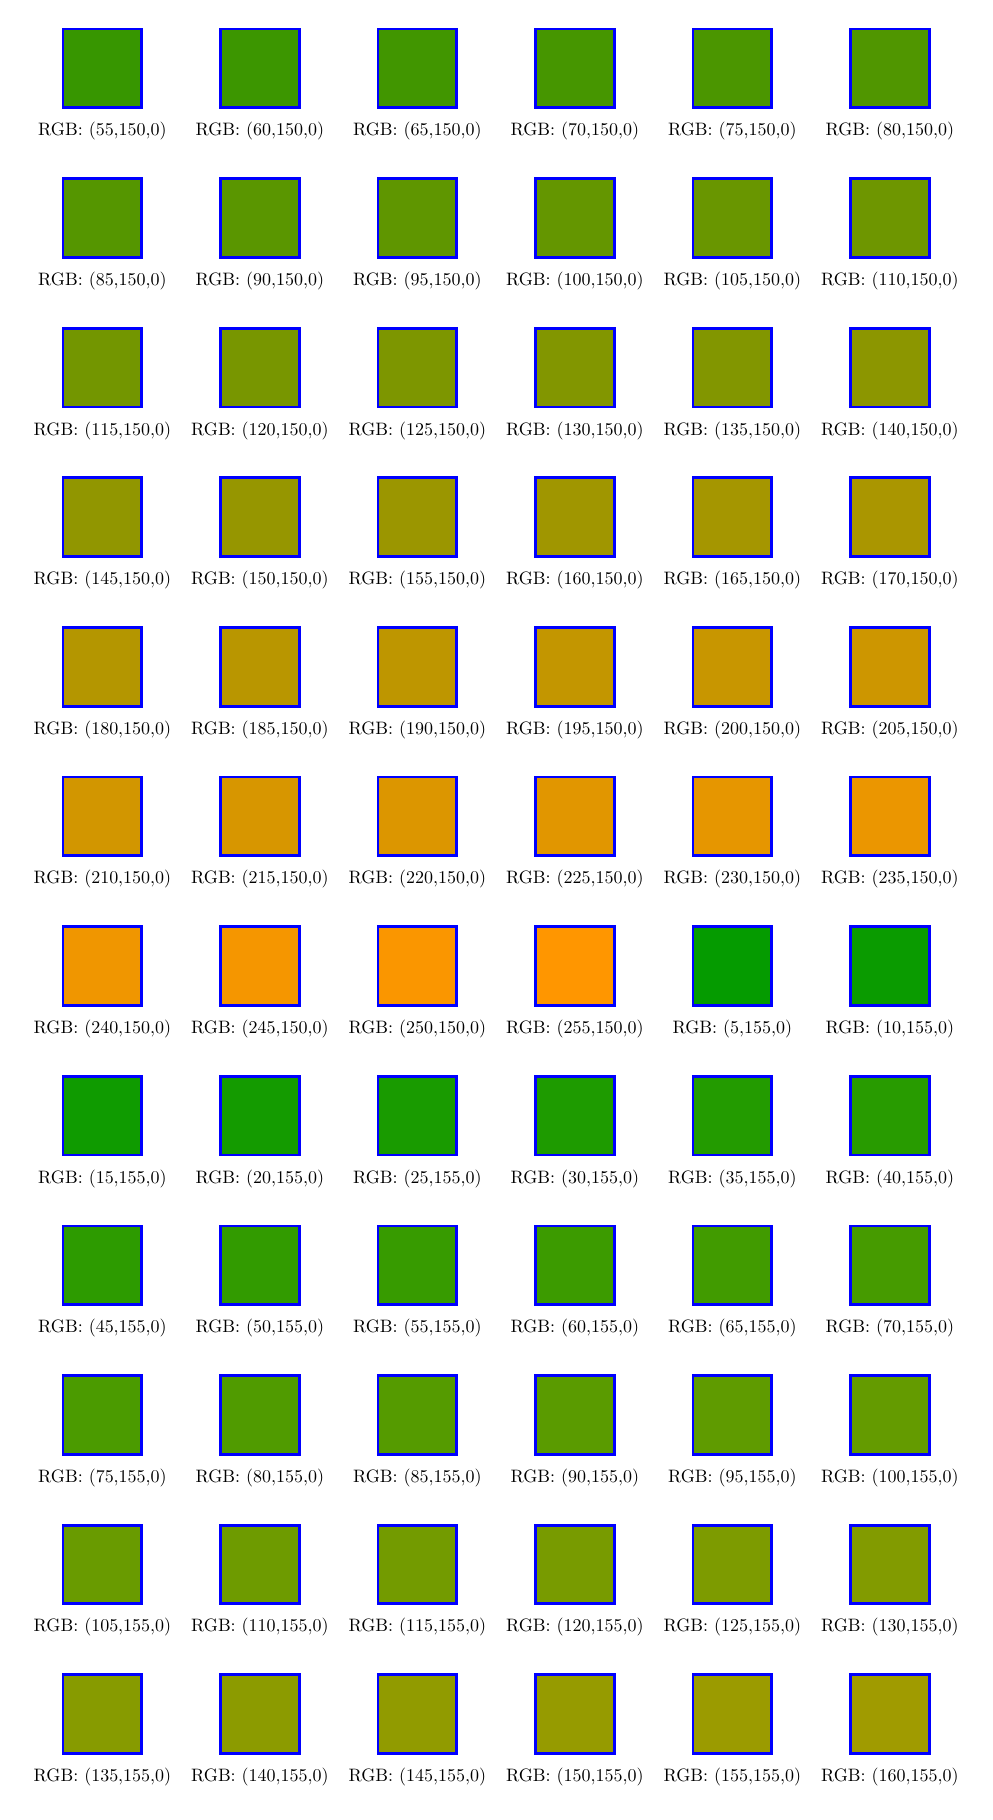
\begin{tikzpicture}

    \filldraw[draw=blue,line width=1,fill=colorR55G150B0]
    (0,0) rectangle (1,1);

    \node[scale=0.65] at (0.5,-0.3) {RGB: (55,150,0)};



    \begin{scope}[xshift=2cm]

      \filldraw[draw=blue,line width=1,fill=colorR60G150B0]
      (0,0) rectangle (1,1);

      \node[scale=0.65] at (0.5,-0.3) {RGB: (60,150,0)};

    \end{scope}



    \begin{scope}[xshift=4cm]

      \filldraw[draw=blue,line width=1,fill=colorR65G150B0]
      (0,0) rectangle (1,1);

      \node[scale=0.65] at (0.5,-0.3) {RGB: (65,150,0)};

    \end{scope}



    \begin{scope}[xshift=6cm]

      \filldraw[draw=blue,line width=1,fill=colorR70G150B0]
      (0,0) rectangle (1,1);

      \node[scale=0.65] at (0.5,-0.3) {RGB: (70,150,0)};

    \end{scope}



    \begin{scope}[xshift=8cm]

      \filldraw[draw=blue,line width=1,fill=colorR75G150B0]
      (0,0) rectangle (1,1);

      \node[scale=0.65] at (0.5,-0.3) {RGB: (75,150,0)};

    \end{scope}



    \begin{scope}[xshift=10cm]

      \filldraw[draw=blue,line width=1,fill=colorR80G150B0]
      (0,0) rectangle (1,1);

      \node[scale=0.65] at (0.5,-0.3) {RGB: (80,150,0)};

    \end{scope}







    \begin{scope}[yshift=-1.9cm]

      \filldraw[draw=blue,line width=1,fill=colorR85G150B0]
      (0,0) rectangle (1,1);

      \node[scale=0.65] at (0.5,-0.3) {RGB: (85,150,0)};

    \end{scope}



    \begin{scope}[xshift=2cm,yshift=-1.9cm]

      \filldraw[draw=blue,line width=1,fill=colorR90G150B0]
      (0,0) rectangle (1,1);

      \node[scale=0.65] at (0.5,-0.3) {RGB: (90,150,0)};

    \end{scope}



    \begin{scope}[xshift=4cm,yshift=-1.9cm]

      \filldraw[draw=blue,line width=1,fill=colorR95G150B0]
      (0,0) rectangle (1,1);

      \node[scale=0.65] at (0.5,-0.3) {RGB: (95,150,0)};

    \end{scope}



    \begin{scope}[xshift=6cm,yshift=-1.9cm]

      \filldraw[draw=blue,line width=1,fill=colorR100G150B0]
      (0,0) rectangle (1,1);

      \node[scale=0.65] at (0.5,-0.3) {RGB: (100,150,0)};

    \end{scope}



    \begin{scope}[xshift=8cm,yshift=-1.9cm]

      \filldraw[draw=blue,line width=1,fill=colorR105G150B0]
      (0,0) rectangle (1,1);

      \node[scale=0.65] at (0.5,-0.3) {RGB: (105,150,0)};

    \end{scope}



    \begin{scope}[xshift=10cm,yshift=-1.9cm]

      \filldraw[draw=blue,line width=1,fill=colorR110G150B0]
      (0,0) rectangle (1,1);

      \node[scale=0.65] at (0.5,-0.3) {RGB: (110,150,0)};

    \end{scope}







    \begin{scope}[yshift=-3.8cm]

      \filldraw[draw=blue,line width=1,fill=colorR115G150B0]
      (0,0) rectangle (1,1);

      \node[scale=0.65] at (0.5,-0.3) {RGB: (115,150,0)};

    \end{scope}



    \begin{scope}[xshift=2cm,yshift=-3.8cm]

      \filldraw[draw=blue,line width=1,fill=colorR120G150B0]
      (0,0) rectangle (1,1);

      \node[scale=0.65] at (0.5,-0.3) {RGB: (120,150,0)};

    \end{scope}



    \begin{scope}[xshift=4cm,yshift=-3.8cm]

      \filldraw[draw=blue,line width=1,fill=colorR125G150B0]
      (0,0) rectangle (1,1);

      \node[scale=0.65] at (0.5,-0.3) {RGB: (125,150,0)};

    \end{scope}



    \begin{scope}[xshift=6cm,yshift=-3.8cm]

      \filldraw[draw=blue,line width=1,fill=colorR130G150B0]
      (0,0) rectangle (1,1);

      \node[scale=0.65] at (0.5,-0.3) {RGB: (130,150,0)};

    \end{scope}



    \begin{scope}[xshift=8cm,yshift=-3.8cm]

      \filldraw[draw=blue,line width=1,fill=colorR130G150B0]
      (0,0) rectangle (1,1);

      \node[scale=0.65] at (0.5,-0.3) {RGB: (135,150,0)};

    \end{scope}



    \begin{scope}[xshift=10cm,yshift=-3.8cm]

      \filldraw[draw=blue,line width=1,fill=colorR140G150B0]
      (0,0) rectangle (1,1);

      \node[scale=0.65] at (0.5,-0.3) {RGB: (140,150,0)};

    \end{scope}







    \begin{scope}[yshift=-5.7cm]

      \filldraw[draw=blue,line width=1,fill=colorR145G150B0]
      (0,0) rectangle (1,1);

      \node[scale=0.65] at (0.5,-0.3) {RGB: (145,150,0)};

    \end{scope}



    \begin{scope}[xshift=2cm,yshift=-5.7cm]

      \filldraw[draw=blue,line width=1,fill=colorR150G150B0]
      (0,0) rectangle (1,1);

      \node[scale=0.65] at (0.5,-0.3) {RGB: (150,150,0)};

    \end{scope}



    \begin{scope}[xshift=4cm,yshift=-5.7cm]

      \filldraw[draw=blue,line width=1,fill=colorR155G150B0]
      (0,0) rectangle (1,1);

      \node[scale=0.65] at (0.5,-0.3) {RGB: (155,150,0)};

    \end{scope}



    \begin{scope}[xshift=6cm,yshift=-5.7cm]

      \filldraw[draw=blue,line width=1,fill=colorR160G150B0]
      (0,0) rectangle (1,1);

      \node[scale=0.65] at (0.5,-0.3) {RGB: (160,150,0)};

    \end{scope}



    \begin{scope}[xshift=8cm,yshift=-5.7cm]

      \filldraw[draw=blue,line width=1,fill=colorR165G150B0]
      (0,0) rectangle (1,1);

      \node[scale=0.65] at (0.5,-0.3) {RGB: (165,150,0)};

    \end{scope}



    \begin{scope}[xshift=10cm,yshift=-5.7cm]

      \filldraw[draw=blue,line width=1,fill=colorR170G150B0]
      (0,0) rectangle (1,1);

      \node[scale=0.65] at (0.5,-0.3) {RGB: (170,150,0)};

    \end{scope}







    \begin{scope}[yshift=-7.6cm]

      \filldraw[draw=blue,line width=1,fill=colorR180G150B0]
      (0,0) rectangle (1,1);

      \node[scale=0.65] at (0.5,-0.3) {RGB: (180,150,0)};

    \end{scope}



    \begin{scope}[xshift=2cm,yshift=-7.6cm]

      \filldraw[draw=blue,line width=1,fill=colorR185G150B0]
      (0,0) rectangle (1,1);

      \node[scale=0.65] at (0.5,-0.3) {RGB: (185,150,0)};

    \end{scope}



    \begin{scope}[xshift=4cm,yshift=-7.6cm]

      \filldraw[draw=blue,line width=1,fill=colorR190G150B0]
      (0,0) rectangle (1,1);

      \node[scale=0.65] at (0.5,-0.3) {RGB: (190,150,0)};

    \end{scope}



    \begin{scope}[xshift=6cm,yshift=-7.6cm]

      \filldraw[draw=blue,line width=1,fill=colorR195G150B0]
      (0,0) rectangle (1,1);

      \node[scale=0.65] at (0.5,-0.3) {RGB: (195,150,0)};

    \end{scope}



    \begin{scope}[xshift=8cm,yshift=-7.6cm]

      \filldraw[draw=blue,line width=1,fill=colorR200G150B0]
      (0,0) rectangle (1,1);

      \node[scale=0.65] at (0.5,-0.3) {RGB: (200,150,0)};

    \end{scope}



    \begin{scope}[xshift=10cm,yshift=-7.6cm]

      \filldraw[draw=blue,line width=1,fill=colorR205G150B0]
      (0,0) rectangle (1,1);

      \node[scale=0.65] at (0.5,-0.3) {RGB: (205,150,0)};

    \end{scope}







    \begin{scope}[yshift=-9.5cm]

      \filldraw[draw=blue,line width=1,fill=colorR210G150B0]
      (0,0) rectangle (1,1);

      \node[scale=0.65] at (0.5,-0.3) {RGB: (210,150,0)};

    \end{scope}



    \begin{scope}[xshift=2cm,yshift=-9.5cm]

      \filldraw[draw=blue,line width=1,fill=colorR215G150B0]
      (0,0) rectangle (1,1);

      \node[scale=0.65] at (0.5,-0.3) {RGB: (215,150,0)};

    \end{scope}



    \begin{scope}[xshift=4cm,yshift=-9.5cm]

      \filldraw[draw=blue,line width=1,fill=colorR220G150B0]
      (0,0) rectangle (1,1);

      \node[scale=0.65] at (0.5,-0.3) {RGB: (220,150,0)};

    \end{scope}



    \begin{scope}[xshift=6cm,yshift=-9.5cm]

      \filldraw[draw=blue,line width=1,fill=colorR225G150B0]
      (0,0) rectangle (1,1);

      \node[scale=0.65] at (0.5,-0.3) {RGB: (225,150,0)};

    \end{scope}



    \begin{scope}[xshift=8cm,yshift=-9.5cm]

      \filldraw[draw=blue,line width=1,fill=colorR230G150B0]
      (0,0) rectangle (1,1);

      \node[scale=0.65] at (0.5,-0.3) {RGB: (230,150,0)};

    \end{scope}



    \begin{scope}[xshift=10cm,yshift=-9.5cm]

      \filldraw[draw=blue,line width=1,fill=colorR235G150B0]
      (0,0) rectangle (1,1);

      \node[scale=0.65] at (0.5,-0.3) {RGB: (235,150,0)};

    \end{scope}







    \begin{scope}[yshift=-11.4cm]

      \filldraw[draw=blue,line width=1,fill=colorR240G150B0]
      (0,0) rectangle (1,1);

      \node[scale=0.65] at (0.5,-0.3) {RGB: (240,150,0)};

    \end{scope}



    \begin{scope}[xshift=2cm,yshift=-11.4cm]

      \filldraw[draw=blue,line width=1,fill=colorR245G150B0]
      (0,0) rectangle (1,1);

      \node[scale=0.65] at (0.5,-0.3) {RGB: (245,150,0)};

    \end{scope}



    \begin{scope}[xshift=4cm,yshift=-11.4cm]

      \filldraw[draw=blue,line width=1,fill=colorR250G150B0]
      (0,0) rectangle (1,1);

      \node[scale=0.65] at (0.5,-0.3) {RGB: (250,150,0)};

    \end{scope}



    \begin{scope}[xshift=6cm,yshift=-11.4cm]

      \filldraw[draw=blue,line width=1,fill=colorR255G150B0]
      (0,0) rectangle (1,1);

      \node[scale=0.65] at (0.5,-0.3) {RGB: (255,150,0)};

    \end{scope}



    \begin{scope}[xshift=8cm,yshift=-11.4cm]

      \filldraw[draw=blue,line width=1,fill=colorR5G155B0]
      (0,0) rectangle (1,1);

      \node[scale=0.65] at (0.5,-0.3) {RGB: (5,155,0)};

    \end{scope}



    \begin{scope}[xshift=10cm,yshift=-11.4cm]

      \filldraw[draw=blue,line width=1,fill=colorR10G155B0]
      (0,0) rectangle (1,1);

      \node[scale=0.65] at (0.5,-0.3) {RGB: (10,155,0)};

    \end{scope}







    \begin{scope}[yshift=-13.3cm]

      \filldraw[draw=blue,line width=1,fill=colorR15G155B0]
      (0,0) rectangle (1,1);

      \node[scale=0.65] at (0.5,-0.3) {RGB: (15,155,0)};

    \end{scope}



    \begin{scope}[xshift=2cm,yshift=-13.3cm]

      \filldraw[draw=blue,line width=1,fill=colorR20G155B0]
      (0,0) rectangle (1,1);

      \node[scale=0.65] at (0.5,-0.3) {RGB: (20,155,0)};

    \end{scope}



    \begin{scope}[xshift=4cm,yshift=-13.3cm]

      \filldraw[draw=blue,line width=1,fill=colorR25G155B0]
      (0,0) rectangle (1,1);

      \node[scale=0.65] at (0.5,-0.3) {RGB: (25,155,0)};

    \end{scope}



    \begin{scope}[xshift=6cm,yshift=-13.3cm]

      \filldraw[draw=blue,line width=1,fill=colorR30G155B0]
      (0,0) rectangle (1,1);

      \node[scale=0.65] at (0.5,-0.3) {RGB: (30,155,0)};

    \end{scope}



    \begin{scope}[xshift=8cm,yshift=-13.3cm]

      \filldraw[draw=blue,line width=1,fill=colorR35G155B0]
      (0,0) rectangle (1,1);

      \node[scale=0.65] at (0.5,-0.3) {RGB: (35,155,0)};

    \end{scope}



    \begin{scope}[xshift=10cm,yshift=-13.3cm]

      \filldraw[draw=blue,line width=1,fill=colorR40G155B0]
      (0,0) rectangle (1,1);

      \node[scale=0.65] at (0.5,-0.3) {RGB: (40,155,0)};

    \end{scope}







    \begin{scope}[yshift=-15.2cm]

      \filldraw[draw=blue,line width=1,fill=colorR45G155B0]
      (0,0) rectangle (1,1);

      \node[scale=0.65] at (0.5,-0.3) {RGB: (45,155,0)};

    \end{scope}



    \begin{scope}[xshift=2cm,yshift=-15.2cm]

      \filldraw[draw=blue,line width=1,fill=colorR50G155B0]
      (0,0) rectangle (1,1);

      \node[scale=0.65] at (0.5,-0.3) {RGB: (50,155,0)};

    \end{scope}



    \begin{scope}[xshift=4cm,yshift=-15.2cm]

      \filldraw[draw=blue,line width=1,fill=colorR55G155B0]
      (0,0) rectangle (1,1);

      \node[scale=0.65] at (0.5,-0.3) {RGB: (55,155,0)};

    \end{scope}



    \begin{scope}[xshift=6cm,yshift=-15.2cm]

      \filldraw[draw=blue,line width=1,fill=colorR60G155B0]
      (0,0) rectangle (1,1);

      \node[scale=0.65] at (0.5,-0.3) {RGB: (60,155,0)};

    \end{scope}



    \begin{scope}[xshift=8cm,yshift=-15.2cm]

      \filldraw[draw=blue,line width=1,fill=colorR65G155B0]
      (0,0) rectangle (1,1);

      \node[scale=0.65] at (0.5,-0.3) {RGB: (65,155,0)};

    \end{scope}



    \begin{scope}[xshift=10cm,yshift=-15.2cm]

      \filldraw[draw=blue,line width=1,fill=colorR70G155B0]
      (0,0) rectangle (1,1);

      \node[scale=0.65] at (0.5,-0.3) {RGB: (70,155,0)};

    \end{scope}







    \begin{scope}[yshift=-17.1cm]

      \filldraw[draw=blue,line width=1,fill=colorR75G155B0]
      (0,0) rectangle (1,1);

      \node[scale=0.65] at (0.5,-0.3) {RGB: (75,155,0)};

    \end{scope}



    \begin{scope}[xshift=2cm,yshift=-17.1cm]

      \filldraw[draw=blue,line width=1,fill=colorR80G155B0]
      (0,0) rectangle (1,1);

      \node[scale=0.65] at (0.5,-0.3) {RGB: (80,155,0)};

    \end{scope}



    \begin{scope}[xshift=4cm,yshift=-17.1cm]

      \filldraw[draw=blue,line width=1,fill=colorR85G155B0]
      (0,0) rectangle (1,1);

      \node[scale=0.65] at (0.5,-0.3) {RGB: (85,155,0)};

    \end{scope}



    \begin{scope}[xshift=6cm,yshift=-17.1cm]

      \filldraw[draw=blue,line width=1,fill=colorR90G155B0]
      (0,0) rectangle (1,1);

      \node[scale=0.65] at (0.5,-0.3) {RGB: (90,155,0)};

    \end{scope}



    \begin{scope}[xshift=8cm,yshift=-17.1cm]

      \filldraw[draw=blue,line width=1,fill=colorR95G155B0]
      (0,0) rectangle (1,1);

      \node[scale=0.65] at (0.5,-0.3) {RGB: (95,155,0)};

    \end{scope}



    \begin{scope}[xshift=10cm,yshift=-17.1cm]

      \filldraw[draw=blue,line width=1,fill=colorR100G155B0]
      (0,0) rectangle (1,1);

      \node[scale=0.65] at (0.5,-0.3) {RGB: (100,155,0)};

    \end{scope}







    \begin{scope}[yshift=-19cm]

      \filldraw[draw=blue,line width=1,fill=colorR105G155B0]
      (0,0) rectangle (1,1);

      \node[scale=0.65] at (0.5,-0.3) {RGB: (105,155,0)};

    \end{scope}



    \begin{scope}[xshift=2cm,yshift=-19cm]

      \filldraw[draw=blue,line width=1,fill=colorR110G155B0]
      (0,0) rectangle (1,1);

      \node[scale=0.65] at (0.5,-0.3) {RGB: (110,155,0)};

    \end{scope}



    \begin{scope}[xshift=4cm,yshift=-19cm]

      \filldraw[draw=blue,line width=1,fill=colorR115G155B0]
      (0,0) rectangle (1,1);

      \node[scale=0.65] at (0.5,-0.3) {RGB: (115,155,0)};

    \end{scope}



    \begin{scope}[xshift=6cm,yshift=-19cm]

      \filldraw[draw=blue,line width=1,fill=colorR120G155B0]
      (0,0) rectangle (1,1);

      \node[scale=0.65] at (0.5,-0.3) {RGB: (120,155,0)};

    \end{scope}



    \begin{scope}[xshift=8cm,yshift=-19cm]

      \filldraw[draw=blue,line width=1,fill=colorR125G155B0]
      (0,0) rectangle (1,1);

      \node[scale=0.65] at (0.5,-0.3) {RGB: (125,155,0)};

    \end{scope}



    \begin{scope}[xshift=10cm,yshift=-19cm]

      \filldraw[draw=blue,line width=1,fill=colorR130G155B0]
      (0,0) rectangle (1,1);

      \node[scale=0.65] at (0.5,-0.3) {RGB: (130,155,0)};

    \end{scope}







    \begin{scope}[yshift=-20.9cm]

      \filldraw[draw=blue,line width=1,fill=colorR135G155B0]
      (0,0) rectangle (1,1);

      \node[scale=0.65] at (0.5,-0.3) {RGB: (135,155,0)};

    \end{scope}



    \begin{scope}[xshift=2cm,yshift=-20.9cm]

      \filldraw[draw=blue,line width=1,fill=colorR140G155B0]
      (0,0) rectangle (1,1);

      \node[scale=0.65] at (0.5,-0.3) {RGB: (140,155,0)};

    \end{scope}



    \begin{scope}[xshift=4cm,yshift=-20.9cm]

      \filldraw[draw=blue,line width=1,fill=colorR145G155B0]
      (0,0) rectangle (1,1);

      \node[scale=0.65] at (0.5,-0.3) {RGB: (145,155,0)};

    \end{scope}



    \begin{scope}[xshift=6cm,yshift=-20.9cm]

      \filldraw[draw=blue,line width=1,fill=colorR150G155B0]
      (0,0) rectangle (1,1);

      \node[scale=0.65] at (0.5,-0.3) {RGB: (150,155,0)};

    \end{scope}



    \begin{scope}[xshift=8cm,yshift=-20.9cm]

      \filldraw[draw=blue,line width=1,fill=colorR155G155B0]
      (0,0) rectangle (1,1);

      \node[scale=0.65] at (0.5,-0.3) {RGB: (155,155,0)};

    \end{scope}



    \begin{scope}[xshift=10cm,yshift=-20.9cm]

      \filldraw[draw=blue,line width=1,fill=colorR160G155B0]
      (0,0) rectangle (1,1);

      \node[scale=0.65] at (0.5,-0.3) {RGB: (160,155,0)};

    \end{scope}

  \end{tikzpicture}

  \caption{Mixed colors in~RGB system: $(55,150,0)$--$(255,150,0)$,
    $(5,155,0)$--$(160,155,0)$}



  \label{fig:Mixed-colors-Part-04}

\end{figure}
% ##################





% ##################
\begin{figure}

  \centering


  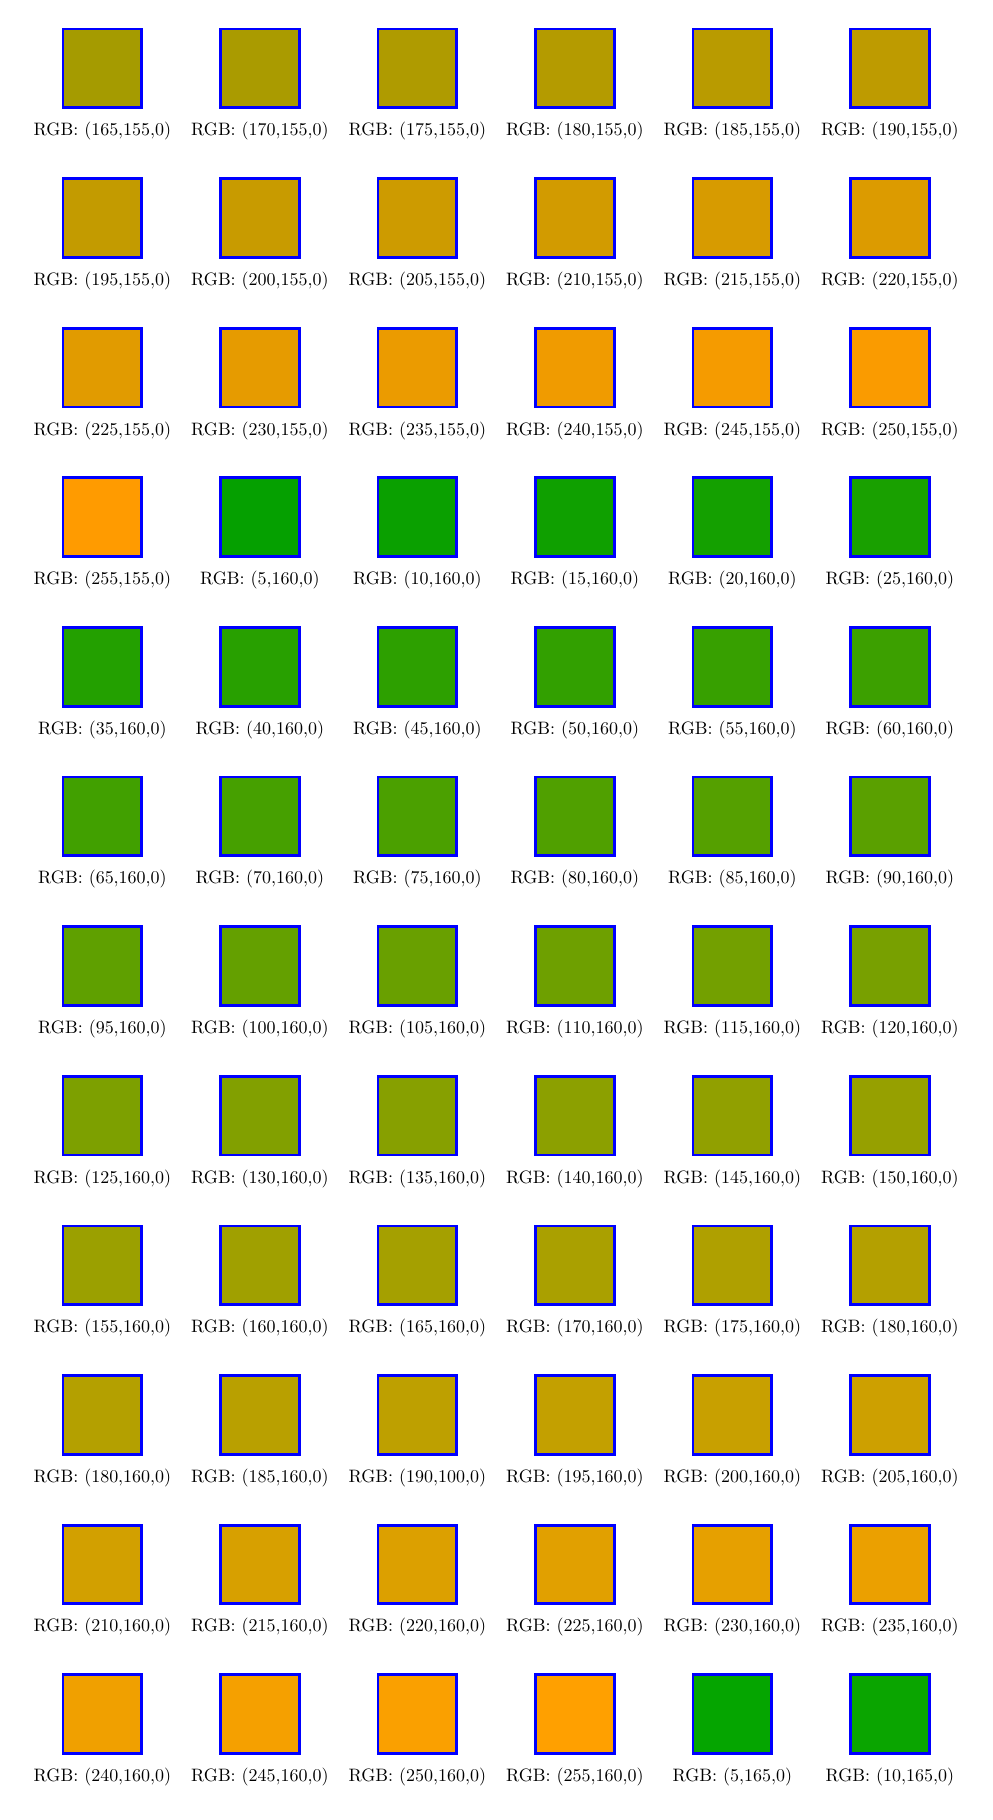
\begin{tikzpicture}

    \filldraw[draw=blue,line width=1,fill=colorR165G155B0]
    (0,0) rectangle (1,1);

    \node[scale=0.65] at (0.5,-0.3) {RGB: (165,155,0)};



    \begin{scope}[xshift=2cm]

      \filldraw[draw=blue,line width=1,fill=colorR170G155B0]
      (0,0) rectangle (1,1);

      \node[scale=0.65] at (0.5,-0.3) {RGB: (170,155,0)};

    \end{scope}



    \begin{scope}[xshift=4cm]

      \filldraw[draw=blue,line width=1,fill=colorR175G155B0]
      (0,0) rectangle (1,1);

      \node[scale=0.65] at (0.5,-0.3) {RGB: (175,155,0)};

    \end{scope}



    \begin{scope}[xshift=6cm]

      \filldraw[draw=blue,line width=1,fill=colorR180G155B0]
      (0,0) rectangle (1,1);

      \node[scale=0.65] at (0.5,-0.3) {RGB: (180,155,0)};

    \end{scope}



    \begin{scope}[xshift=8cm]

      \filldraw[draw=blue,line width=1,fill=colorR185G155B0]
      (0,0) rectangle (1,1);

      \node[scale=0.65] at (0.5,-0.3) {RGB: (185,155,0)};

    \end{scope}



    \begin{scope}[xshift=10cm]

      \filldraw[draw=blue,line width=1,fill=colorR190G155B0]
      (0,0) rectangle (1,1);

      \node[scale=0.65] at (0.5,-0.3) {RGB: (190,155,0)};

    \end{scope}







    \begin{scope}[yshift=-1.9cm]

      \filldraw[draw=blue,line width=1,fill=colorR195G155B0]
      (0,0) rectangle (1,1);

      \node[scale=0.65] at (0.5,-0.3) {RGB: (195,155,0)};

    \end{scope}



    \begin{scope}[xshift=2cm,yshift=-1.9cm]

      \filldraw[draw=blue,line width=1,fill=colorR200G155B0]
      (0,0) rectangle (1,1);

      \node[scale=0.65] at (0.5,-0.3) {RGB: (200,155,0)};

    \end{scope}



    \begin{scope}[xshift=4cm,yshift=-1.9cm]

      \filldraw[draw=blue,line width=1,fill=colorR205G155B0]
      (0,0) rectangle (1,1);

      \node[scale=0.65] at (0.5,-0.3) {RGB: (205,155,0)};

    \end{scope}



    \begin{scope}[xshift=6cm,yshift=-1.9cm]

      \filldraw[draw=blue,line width=1,fill=colorR210G155B0]
      (0,0) rectangle (1,1);

      \node[scale=0.65] at (0.5,-0.3) {RGB: (210,155,0)};

    \end{scope}



    \begin{scope}[xshift=8cm,yshift=-1.9cm]

      \filldraw[draw=blue,line width=1,fill=colorR215G155B0]
      (0,0) rectangle (1,1);

      \node[scale=0.65] at (0.5,-0.3) {RGB: (215,155,0)};

    \end{scope}



    \begin{scope}[xshift=10cm,yshift=-1.9cm]

      \filldraw[draw=blue,line width=1,fill=colorR220G155B0]
      (0,0) rectangle (1,1);

      \node[scale=0.65] at (0.5,-0.3) {RGB: (220,155,0)};

    \end{scope}







    \begin{scope}[yshift=-3.8cm]

      \filldraw[draw=blue,line width=1,fill=colorR225G155B0]
      (0,0) rectangle (1,1);

      \node[scale=0.65] at (0.5,-0.3) {RGB: (225,155,0)};

    \end{scope}



    \begin{scope}[xshift=2cm,yshift=-3.8cm]

      \filldraw[draw=blue,line width=1,fill=colorR230G155B0]
      (0,0) rectangle (1,1);

      \node[scale=0.65] at (0.5,-0.3) {RGB: (230,155,0)};

    \end{scope}



    \begin{scope}[xshift=4cm,yshift=-3.8cm]

      \filldraw[draw=blue,line width=1,fill=colorR235G155B0]
      (0,0) rectangle (1,1);

      \node[scale=0.65] at (0.5,-0.3) {RGB: (235,155,0)};

    \end{scope}



    \begin{scope}[xshift=6cm,yshift=-3.8cm]

      \filldraw[draw=blue,line width=1,fill=colorR240G155B0]
      (0,0) rectangle (1,1);

      \node[scale=0.65] at (0.5,-0.3) {RGB: (240,155,0)};

    \end{scope}



    \begin{scope}[xshift=8cm,yshift=-3.8cm]

      \filldraw[draw=blue,line width=1,fill=colorR245G155B0]
      (0,0) rectangle (1,1);

      \node[scale=0.65] at (0.5,-0.3) {RGB: (245,155,0)};

    \end{scope}



    \begin{scope}[xshift=10cm,yshift=-3.8cm]

      \filldraw[draw=blue,line width=1,fill=colorR250G155B0]
      (0,0) rectangle (1,1);

      \node[scale=0.65] at (0.5,-0.3) {RGB: (250,155,0)};

    \end{scope}







    \begin{scope}[yshift=-5.7cm]

      \filldraw[draw=blue,line width=1,fill=colorR255G155B0]
      (0,0) rectangle (1,1);

      \node[scale=0.65] at (0.5,-0.3) {RGB: (255,155,0)};

    \end{scope}



    \begin{scope}[xshift=2cm,yshift=-5.7cm]

      \filldraw[draw=blue,line width=1,fill=colorR5G160B0]
      (0,0) rectangle (1,1);

      \node[scale=0.65] at (0.5,-0.3) {RGB: (5,160,0)};

    \end{scope}



    \begin{scope}[xshift=4cm,yshift=-5.7cm]

      \filldraw[draw=blue,line width=1,fill=colorR10G160B0]
      (0,0) rectangle (1,1);

      \node[scale=0.65] at (0.5,-0.3) {RGB: (10,160,0)};

    \end{scope}



    \begin{scope}[xshift=6cm,yshift=-5.7cm]

      \filldraw[draw=blue,line width=1,fill=colorR15G160B0]
      (0,0) rectangle (1,1);

      \node[scale=0.65] at (0.5,-0.3) {RGB: (15,160,0)};

    \end{scope}



    \begin{scope}[xshift=8cm,yshift=-5.7cm]

      \filldraw[draw=blue,line width=1,fill=colorR20G160B0]
      (0,0) rectangle (1,1);

      \node[scale=0.65] at (0.5,-0.3) {RGB: (20,160,0)};

    \end{scope}



    \begin{scope}[xshift=10cm,yshift=-5.7cm]

      \filldraw[draw=blue,line width=1,fill=colorR25G160B0]
      (0,0) rectangle (1,1);

      \node[scale=0.65] at (0.5,-0.3) {RGB: (25,160,0)};

    \end{scope}







    \begin{scope}[yshift=-7.6cm]

      \filldraw[draw=blue,line width=1,fill=colorR35G160B0]
      (0,0) rectangle (1,1);

      \node[scale=0.65] at (0.5,-0.3) {RGB: (35,160,0)};

    \end{scope}



    \begin{scope}[xshift=2cm,yshift=-7.6cm]

      \filldraw[draw=blue,line width=1,fill=colorR40G160B0]
      (0,0) rectangle (1,1);

      \node[scale=0.65] at (0.5,-0.3) {RGB: (40,160,0)};

    \end{scope}



    \begin{scope}[xshift=4cm,yshift=-7.6cm]

      \filldraw[draw=blue,line width=1,fill=colorR45G160B0]
      (0,0) rectangle (1,1);

      \node[scale=0.65] at (0.5,-0.3) {RGB: (45,160,0)};

    \end{scope}



    \begin{scope}[xshift=6cm,yshift=-7.6cm]

      \filldraw[draw=blue,line width=1,fill=colorR50G160B0]
      (0,0) rectangle (1,1);

      \node[scale=0.65] at (0.5,-0.3) {RGB: (50,160,0)};

    \end{scope}



    \begin{scope}[xshift=8cm,yshift=-7.6cm]

      \filldraw[draw=blue,line width=1,fill=colorR55G160B0]
      (0,0) rectangle (1,1);

      \node[scale=0.65] at (0.5,-0.3) {RGB: (55,160,0)};

    \end{scope}



    \begin{scope}[xshift=10cm,yshift=-7.6cm]

      \filldraw[draw=blue,line width=1,fill=colorR60G160B0]
      (0,0) rectangle (1,1);

      \node[scale=0.65] at (0.5,-0.3) {RGB: (60,160,0)};

    \end{scope}







    \begin{scope}[yshift=-9.5cm]

      \filldraw[draw=blue,line width=1,fill=colorR65G160B0]
      (0,0) rectangle (1,1);

      \node[scale=0.65] at (0.5,-0.3) {RGB: (65,160,0)};

    \end{scope}



    \begin{scope}[xshift=2cm,yshift=-9.5cm]

      \filldraw[draw=blue,line width=1,fill=colorR70G160B0]
      (0,0) rectangle (1,1);

      \node[scale=0.65] at (0.5,-0.3) {RGB: (70,160,0)};

    \end{scope}



    \begin{scope}[xshift=4cm,yshift=-9.5cm]

      \filldraw[draw=blue,line width=1,fill=colorR75G160B0]
      (0,0) rectangle (1,1);

      \node[scale=0.65] at (0.5,-0.3) {RGB: (75,160,0)};

    \end{scope}



    \begin{scope}[xshift=6cm,yshift=-9.5cm]

      \filldraw[draw=blue,line width=1,fill=colorR80G160B0]
      (0,0) rectangle (1,1);

      \node[scale=0.65] at (0.5,-0.3) {RGB: (80,160,0)};

    \end{scope}



    \begin{scope}[xshift=8cm,yshift=-9.5cm]

      \filldraw[draw=blue,line width=1,fill=colorR85G160B0]
      (0,0) rectangle (1,1);

      \node[scale=0.65] at (0.5,-0.3) {RGB: (85,160,0)};

    \end{scope}



    \begin{scope}[xshift=10cm,yshift=-9.5cm]

      \filldraw[draw=blue,line width=1,fill=colorR90G160B0]
      (0,0) rectangle (1,1);

      \node[scale=0.65] at (0.5,-0.3) {RGB: (90,160,0)};

    \end{scope}







    \begin{scope}[yshift=-11.4cm]

      \filldraw[draw=blue,line width=1,fill=colorR95G160B0]
      (0,0) rectangle (1,1);

      \node[scale=0.65] at (0.5,-0.3) {RGB: (95,160,0)};

    \end{scope}



    \begin{scope}[xshift=2cm,yshift=-11.4cm]

      \filldraw[draw=blue,line width=1,fill=colorR100G160B0]
      (0,0) rectangle (1,1);

      \node[scale=0.65] at (0.5,-0.3) {RGB: (100,160,0)};

    \end{scope}



    \begin{scope}[xshift=4cm,yshift=-11.4cm]

      \filldraw[draw=blue,line width=1,fill=colorR105G160B0]
      (0,0) rectangle (1,1);

      \node[scale=0.65] at (0.5,-0.3) {RGB: (105,160,0)};

    \end{scope}



    \begin{scope}[xshift=6cm,yshift=-11.4cm]

      \filldraw[draw=blue,line width=1,fill=colorR110G160B0]
      (0,0) rectangle (1,1);

      \node[scale=0.65] at (0.5,-0.3) {RGB: (110,160,0)};

    \end{scope}



    \begin{scope}[xshift=8cm,yshift=-11.4cm]

      \filldraw[draw=blue,line width=1,fill=colorR115G160B0]
      (0,0) rectangle (1,1);

      \node[scale=0.65] at (0.5,-0.3) {RGB: (115,160,0)};

    \end{scope}



    \begin{scope}[xshift=10cm,yshift=-11.4cm]

      \filldraw[draw=blue,line width=1,fill=colorR120G160B0]
      (0,0) rectangle (1,1);

      \node[scale=0.65] at (0.5,-0.3) {RGB: (120,160,0)};

    \end{scope}







    \begin{scope}[yshift=-13.3cm]

      \filldraw[draw=blue,line width=1,fill=colorR125G160B0]
      (0,0) rectangle (1,1);

      \node[scale=0.65] at (0.5,-0.3) {RGB: (125,160,0)};

    \end{scope}



    \begin{scope}[xshift=2cm,yshift=-13.3cm]

      \filldraw[draw=blue,line width=1,fill=colorR130G160B0]
      (0,0) rectangle (1,1);

      \node[scale=0.65] at (0.5,-0.3) {RGB: (130,160,0)};

    \end{scope}



    \begin{scope}[xshift=4cm,yshift=-13.3cm]

      \filldraw[draw=blue,line width=1,fill=colorR135G160B0]
      (0,0) rectangle (1,1);

      \node[scale=0.65] at (0.5,-0.3) {RGB: (135,160,0)};

    \end{scope}



    \begin{scope}[xshift=6cm,yshift=-13.3cm]

      \filldraw[draw=blue,line width=1,fill=colorR140G160B0]
      (0,0) rectangle (1,1);

      \node[scale=0.65] at (0.5,-0.3) {RGB: (140,160,0)};

    \end{scope}



    \begin{scope}[xshift=8cm,yshift=-13.3cm]

      \filldraw[draw=blue,line width=1,fill=colorR145G160B0]
      (0,0) rectangle (1,1);

      \node[scale=0.65] at (0.5,-0.3) {RGB: (145,160,0)};

    \end{scope}



    \begin{scope}[xshift=10cm,yshift=-13.3cm]

      \filldraw[draw=blue,line width=1,fill=colorR150G160B0]
      (0,0) rectangle (1,1);

      \node[scale=0.65] at (0.5,-0.3) {RGB: (150,160,0)};

    \end{scope}







    \begin{scope}[yshift=-15.2cm]

      \filldraw[draw=blue,line width=1,fill=colorR155G160B0]
      (0,0) rectangle (1,1);

      \node[scale=0.65] at (0.5,-0.3) {RGB: (155,160,0)};

    \end{scope}



    \begin{scope}[xshift=2cm,yshift=-15.2cm]

      \filldraw[draw=blue,line width=1,fill=colorR160G160B0]
      (0,0) rectangle (1,1);

      \node[scale=0.65] at (0.5,-0.3) {RGB: (160,160,0)};

    \end{scope}



    \begin{scope}[xshift=4cm,yshift=-15.2cm]

      \filldraw[draw=blue,line width=1,fill=colorR165G160B0]
      (0,0) rectangle (1,1);

      \node[scale=0.65] at (0.5,-0.3) {RGB: (165,160,0)};

    \end{scope}



    \begin{scope}[xshift=6cm,yshift=-15.2cm]

      \filldraw[draw=blue,line width=1,fill=colorR170G160B0]
      (0,0) rectangle (1,1);

      \node[scale=0.65] at (0.5,-0.3) {RGB: (170,160,0)};

    \end{scope}



    \begin{scope}[xshift=8cm,yshift=-15.2cm]

      \filldraw[draw=blue,line width=1,fill=colorR175G160B0]
      (0,0) rectangle (1,1);

      \node[scale=0.65] at (0.5,-0.3) {RGB: (175,160,0)};

    \end{scope}



    \begin{scope}[xshift=10cm,yshift=-15.2cm]

      \filldraw[draw=blue,line width=1,fill=colorR180G160B0]
      (0,0) rectangle (1,1);

      \node[scale=0.65] at (0.5,-0.3) {RGB: (180,160,0)};

    \end{scope}







    \begin{scope}[yshift=-17.1cm]

      \filldraw[draw=blue,line width=1,fill=colorR180G160B0]
      (0,0) rectangle (1,1);

      \node[scale=0.65] at (0.5,-0.3) {RGB: (180,160,0)};

    \end{scope}



    \begin{scope}[xshift=2cm,yshift=-17.1cm]

      \filldraw[draw=blue,line width=1,fill=colorR185G160B0]
      (0,0) rectangle (1,1);

      \node[scale=0.65] at (0.5,-0.3) {RGB: (185,160,0)};

    \end{scope}



    \begin{scope}[xshift=4cm,yshift=-17.1cm]

      \filldraw[draw=blue,line width=1,fill=colorR190G160B0]
      (0,0) rectangle (1,1);

      \node[scale=0.65] at (0.5,-0.3) {RGB: (190,100,0)};

    \end{scope}



    \begin{scope}[xshift=6cm,yshift=-17.1cm]

      \filldraw[draw=blue,line width=1,fill=colorR195G160B0]
      (0,0) rectangle (1,1);

      \node[scale=0.65] at (0.5,-0.3) {RGB: (195,160,0)};

    \end{scope}



    \begin{scope}[xshift=8cm,yshift=-17.1cm]

      \filldraw[draw=blue,line width=1,fill=colorR200G160B0]
      (0,0) rectangle (1,1);

      \node[scale=0.65] at (0.5,-0.3) {RGB: (200,160,0)};

    \end{scope}



    \begin{scope}[xshift=10cm,yshift=-17.1cm]

      \filldraw[draw=blue,line width=1,fill=colorR205G160B0]
      (0,0) rectangle (1,1);

      \node[scale=0.65] at (0.5,-0.3) {RGB: (205,160,0)};

    \end{scope}







    \begin{scope}[yshift=-19cm]

      \filldraw[draw=blue,line width=1,fill=colorR210G160B0]
      (0,0) rectangle (1,1);

      \node[scale=0.65] at (0.5,-0.3) {RGB: (210,160,0)};

    \end{scope}



    \begin{scope}[xshift=2cm,yshift=-19cm]

      \filldraw[draw=blue,line width=1,fill=colorR215G160B0]
      (0,0) rectangle (1,1);

      \node[scale=0.65] at (0.5,-0.3) {RGB: (215,160,0)};

    \end{scope}



    \begin{scope}[xshift=4cm,yshift=-19cm]

      \filldraw[draw=blue,line width=1,fill=colorR220G160B0]
      (0,0) rectangle (1,1);

      \node[scale=0.65] at (0.5,-0.3) {RGB: (220,160,0)};

    \end{scope}



    \begin{scope}[xshift=6cm,yshift=-19cm]

      \filldraw[draw=blue,line width=1,fill=colorR225G160B0]
      (0,0) rectangle (1,1);

      \node[scale=0.65] at (0.5,-0.3) {RGB: (225,160,0)};

    \end{scope}



    \begin{scope}[xshift=8cm,yshift=-19cm]

      \filldraw[draw=blue,line width=1,fill=colorR230G160B0]
      (0,0) rectangle (1,1);

      \node[scale=0.65] at (0.5,-0.3) {RGB: (230,160,0)};

    \end{scope}



    \begin{scope}[xshift=10cm,yshift=-19cm]

      \filldraw[draw=blue,line width=1,fill=colorR235G160B0]
      (0,0) rectangle (1,1);

      \node[scale=0.65] at (0.5,-0.3) {RGB: (235,160,0)};

    \end{scope}







    \begin{scope}[yshift=-20.9cm]

      \filldraw[draw=blue,line width=1,fill=colorR240G160B0]
      (0,0) rectangle (1,1);

      \node[scale=0.65] at (0.5,-0.3) {RGB: (240,160,0)};

    \end{scope}



    \begin{scope}[xshift=2cm,yshift=-20.9cm]

      \filldraw[draw=blue,line width=1,fill=colorR245G160B0]
      (0,0) rectangle (1,1);

      \node[scale=0.65] at (0.5,-0.3) {RGB: (245,160,0)};

    \end{scope}



    \begin{scope}[xshift=4cm,yshift=-20.9cm]

      \filldraw[draw=blue,line width=1,fill=colorR250G160B0]
      (0,0) rectangle (1,1);

      \node[scale=0.65] at (0.5,-0.3) {RGB: (250,160,0)};

    \end{scope}



    \begin{scope}[xshift=6cm,yshift=-20.9cm]

      \filldraw[draw=blue,line width=1,fill=colorR255G160B0]
      (0,0) rectangle (1,1);

      \node[scale=0.65] at (0.5,-0.3) {RGB: (255,160,0)};

    \end{scope}



    \begin{scope}[xshift=8cm,yshift=-20.9cm]

      \filldraw[draw=blue,line width=1,fill=colorR5G165B0]
      (0,0) rectangle (1,1);

      \node[scale=0.65] at (0.5,-0.3) {RGB: (5,165,0)};

    \end{scope}



    \begin{scope}[xshift=10cm,yshift=-20.9cm]

      \filldraw[draw=blue,line width=1,fill=colorR10G165B0]
      (0,0) rectangle (1,1);

      \node[scale=0.65] at (0.5,-0.3) {RGB: (10,165,0)};

    \end{scope}

  \end{tikzpicture}

  \caption{Mixed colors in~RGB system: $(165,155,0)$--$(255,155,0)$,
    $(5,160,0)$--$(255,160,0)$, $(5,165,0)$--$(10,165,0)$}



  \label{fig:Mixed-colors-Part-05}

\end{figure}
% ##################





% ##################
\begin{figure}

  \centering


  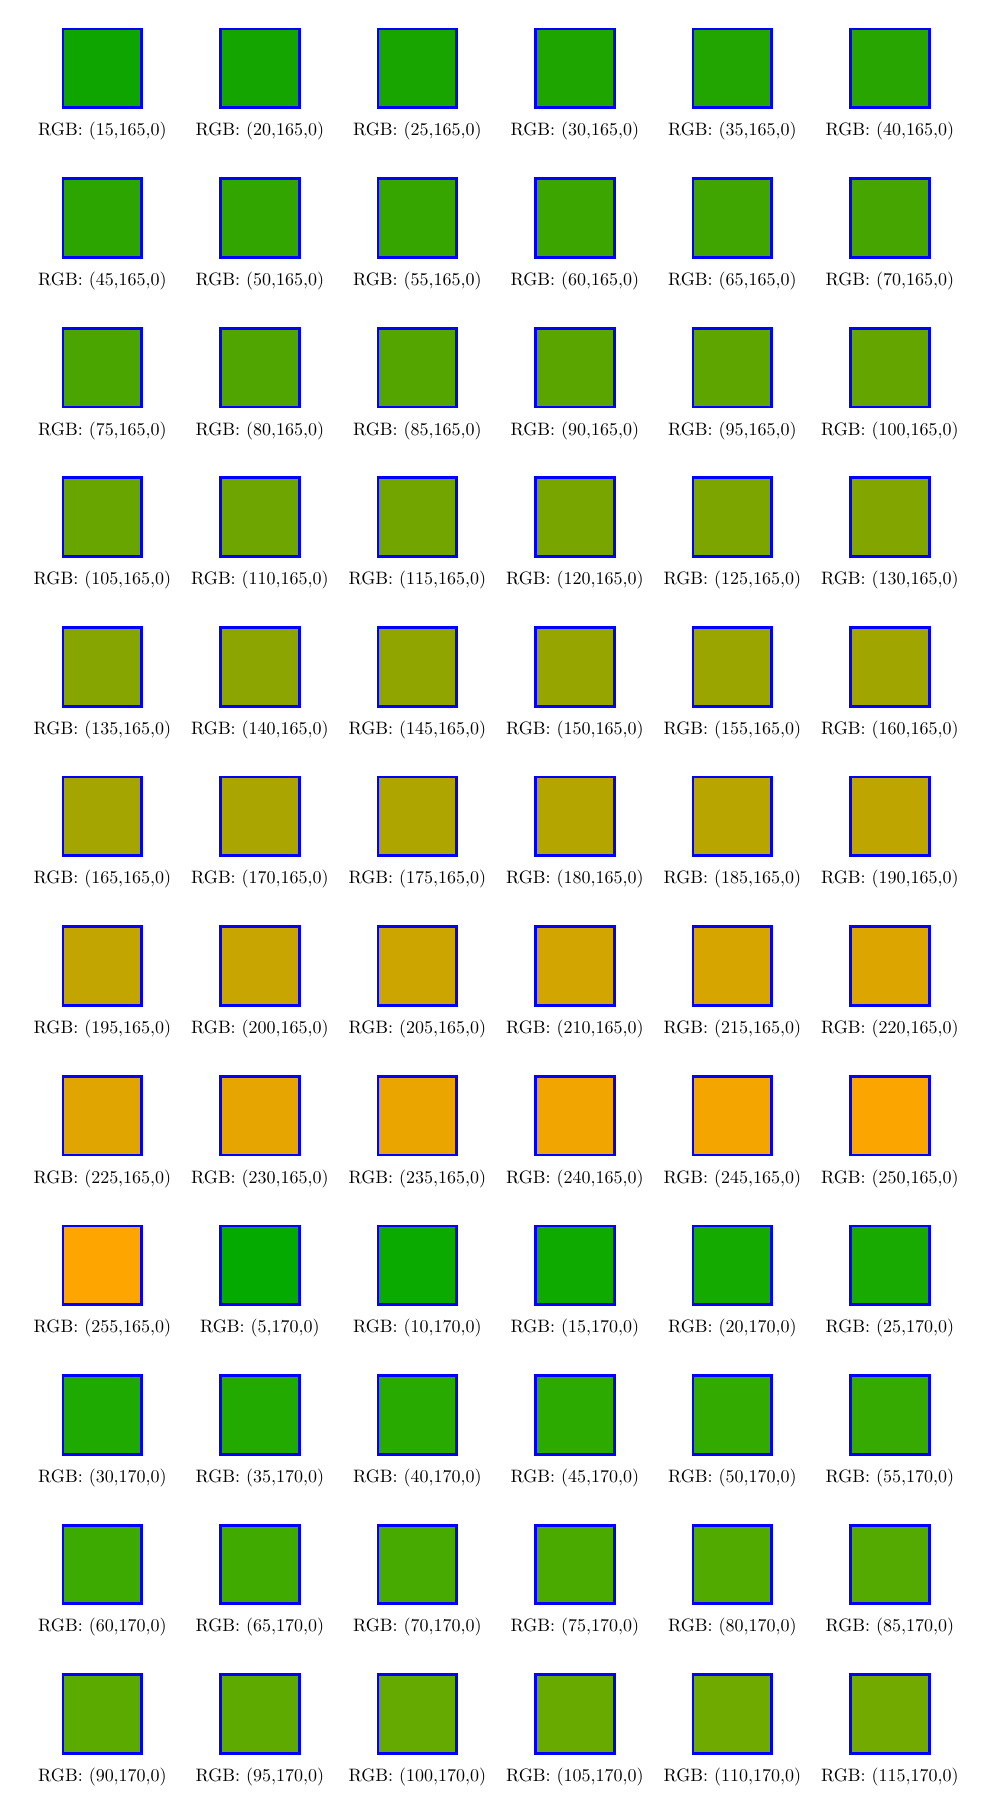
\begin{tikzpicture}

    \filldraw[draw=blue,line width=1,fill=colorR15G165B0]
    (0,0) rectangle (1,1);

    \node[scale=0.65] at (0.5,-0.3) {RGB: (15,165,0)};



    \begin{scope}[xshift=2cm]

      \filldraw[draw=blue,line width=1,fill=colorR20G165B0]
      (0,0) rectangle (1,1);

      \node[scale=0.65] at (0.5,-0.3) {RGB: (20,165,0)};

    \end{scope}



    \begin{scope}[xshift=4cm]

      \filldraw[draw=blue,line width=1,fill=colorR25G165B0]
      (0,0) rectangle (1,1);

      \node[scale=0.65] at (0.5,-0.3) {RGB: (25,165,0)};

    \end{scope}



    \begin{scope}[xshift=6cm]

      \filldraw[draw=blue,line width=1,fill=colorR30G165B0]
      (0,0) rectangle (1,1);

      \node[scale=0.65] at (0.5,-0.3) {RGB: (30,165,0)};

    \end{scope}



    \begin{scope}[xshift=8cm]

      \filldraw[draw=blue,line width=1,fill=colorR35G165B0]
      (0,0) rectangle (1,1);

      \node[scale=0.65] at (0.5,-0.3) {RGB: (35,165,0)};

    \end{scope}



    \begin{scope}[xshift=10cm]

      \filldraw[draw=blue,line width=1,fill=colorR40G165B0]
      (0,0) rectangle (1,1);

      \node[scale=0.65] at (0.5,-0.3) {RGB: (40,165,0)};

    \end{scope}







    \begin{scope}[yshift=-1.9cm]

      \filldraw[draw=blue,line width=1,fill=colorR45G165B0]
      (0,0) rectangle (1,1);

      \node[scale=0.65] at (0.5,-0.3) {RGB: (45,165,0)};

    \end{scope}



    \begin{scope}[xshift=2cm,yshift=-1.9cm]

      \filldraw[draw=blue,line width=1,fill=colorR50G165B0]
      (0,0) rectangle (1,1);

      \node[scale=0.65] at (0.5,-0.3) {RGB: (50,165,0)};

    \end{scope}



    \begin{scope}[xshift=4cm,yshift=-1.9cm]

      \filldraw[draw=blue,line width=1,fill=colorR55G165B0]
      (0,0) rectangle (1,1);

      \node[scale=0.65] at (0.5,-0.3) {RGB: (55,165,0)};

    \end{scope}



    \begin{scope}[xshift=6cm,yshift=-1.9cm]

      \filldraw[draw=blue,line width=1,fill=colorR60G165B0]
      (0,0) rectangle (1,1);

      \node[scale=0.65] at (0.5,-0.3) {RGB: (60,165,0)};

    \end{scope}



    \begin{scope}[xshift=8cm,yshift=-1.9cm]

      \filldraw[draw=blue,line width=1,fill=colorR65G165B0]
      (0,0) rectangle (1,1);

      \node[scale=0.65] at (0.5,-0.3) {RGB: (65,165,0)};

    \end{scope}



    \begin{scope}[xshift=10cm,yshift=-1.9cm]

      \filldraw[draw=blue,line width=1,fill=colorR70G165B0]
      (0,0) rectangle (1,1);

      \node[scale=0.65] at (0.5,-0.3) {RGB: (70,165,0)};

    \end{scope}







    \begin{scope}[yshift=-3.8cm]

      \filldraw[draw=blue,line width=1,fill=colorR75G165B0]
      (0,0) rectangle (1,1);

      \node[scale=0.65] at (0.5,-0.3) {RGB: (75,165,0)};

    \end{scope}



    \begin{scope}[xshift=2cm,yshift=-3.8cm]

      \filldraw[draw=blue,line width=1,fill=colorR80G165B0]
      (0,0) rectangle (1,1);

      \node[scale=0.65] at (0.5,-0.3) {RGB: (80,165,0)};

    \end{scope}



    \begin{scope}[xshift=4cm,yshift=-3.8cm]

      \filldraw[draw=blue,line width=1,fill=colorR85G165B0]
      (0,0) rectangle (1,1);

      \node[scale=0.65] at (0.5,-0.3) {RGB: (85,165,0)};

    \end{scope}



    \begin{scope}[xshift=6cm,yshift=-3.8cm]

      \filldraw[draw=blue,line width=1,fill=colorR90G165B0]
      (0,0) rectangle (1,1);

      \node[scale=0.65] at (0.5,-0.3) {RGB: (90,165,0)};

    \end{scope}



    \begin{scope}[xshift=8cm,yshift=-3.8cm]

      \filldraw[draw=blue,line width=1,fill=colorR95G165B0]
      (0,0) rectangle (1,1);

      \node[scale=0.65] at (0.5,-0.3) {RGB: (95,165,0)};

    \end{scope}



    \begin{scope}[xshift=10cm,yshift=-3.8cm]

      \filldraw[draw=blue,line width=1,fill=colorR100G165B0]
      (0,0) rectangle (1,1);

      \node[scale=0.65] at (0.5,-0.3) {RGB: (100,165,0)};

    \end{scope}







    \begin{scope}[yshift=-5.7cm]

      \filldraw[draw=blue,line width=1,fill=colorR105G165B0]
      (0,0) rectangle (1,1);

      \node[scale=0.65] at (0.5,-0.3) {RGB: (105,165,0)};

    \end{scope}



    \begin{scope}[xshift=2cm,yshift=-5.7cm]

      \filldraw[draw=blue,line width=1,fill=colorR110G165B0]
      (0,0) rectangle (1,1);

      \node[scale=0.65] at (0.5,-0.3) {RGB: (110,165,0)};

    \end{scope}



    \begin{scope}[xshift=4cm,yshift=-5.7cm]

      \filldraw[draw=blue,line width=1,fill=colorR115G165B0]
      (0,0) rectangle (1,1);

      \node[scale=0.65] at (0.5,-0.3) {RGB: (115,165,0)};

    \end{scope}



    \begin{scope}[xshift=6cm,yshift=-5.7cm]

      \filldraw[draw=blue,line width=1,fill=colorR120G165B0]
      (0,0) rectangle (1,1);

      \node[scale=0.65] at (0.5,-0.3) {RGB: (120,165,0)};

    \end{scope}



    \begin{scope}[xshift=8cm,yshift=-5.7cm]

      \filldraw[draw=blue,line width=1,fill=colorR125G165B0]
      (0,0) rectangle (1,1);

      \node[scale=0.65] at (0.5,-0.3) {RGB: (125,165,0)};

    \end{scope}



    \begin{scope}[xshift=10cm,yshift=-5.7cm]

      \filldraw[draw=blue,line width=1,fill=colorR130G165B0]
      (0,0) rectangle (1,1);

      \node[scale=0.65] at (0.5,-0.3) {RGB: (130,165,0)};

    \end{scope}







    \begin{scope}[yshift=-7.6cm]

      \filldraw[draw=blue,line width=1,fill=colorR135G165B0]
      (0,0) rectangle (1,1);

      \node[scale=0.65] at (0.5,-0.3) {RGB: (135,165,0)};

    \end{scope}



    \begin{scope}[xshift=2cm,yshift=-7.6cm]

      \filldraw[draw=blue,line width=1,fill=colorR140G165B0]
      (0,0) rectangle (1,1);

      \node[scale=0.65] at (0.5,-0.3) {RGB: (140,165,0)};

    \end{scope}



    \begin{scope}[xshift=4cm,yshift=-7.6cm]

      \filldraw[draw=blue,line width=1,fill=colorR145G165B0]
      (0,0) rectangle (1,1);

      \node[scale=0.65] at (0.5,-0.3) {RGB: (145,165,0)};

    \end{scope}



    \begin{scope}[xshift=6cm,yshift=-7.6cm]

      \filldraw[draw=blue,line width=1,fill=colorR150G165B0]
      (0,0) rectangle (1,1);

      \node[scale=0.65] at (0.5,-0.3) {RGB: (150,165,0)};

    \end{scope}



    \begin{scope}[xshift=8cm,yshift=-7.6cm]

      \filldraw[draw=blue,line width=1,fill=colorR155G165B0]
      (0,0) rectangle (1,1);

      \node[scale=0.65] at (0.5,-0.3) {RGB: (155,165,0)};

    \end{scope}



    \begin{scope}[xshift=10cm,yshift=-7.6cm]

      \filldraw[draw=blue,line width=1,fill=colorR160G165B0]
      (0,0) rectangle (1,1);

      \node[scale=0.65] at (0.5,-0.3) {RGB: (160,165,0)};

    \end{scope}







    \begin{scope}[yshift=-9.5cm]

      \filldraw[draw=blue,line width=1,fill=colorR165G165B0]
      (0,0) rectangle (1,1);

      \node[scale=0.65] at (0.5,-0.3) {RGB: (165,165,0)};

    \end{scope}



    \begin{scope}[xshift=2cm,yshift=-9.5cm]

      \filldraw[draw=blue,line width=1,fill=colorR170G165B0]
      (0,0) rectangle (1,1);

      \node[scale=0.65] at (0.5,-0.3) {RGB: (170,165,0)};

    \end{scope}



    \begin{scope}[xshift=4cm,yshift=-9.5cm]

      \filldraw[draw=blue,line width=1,fill=colorR175G165B0]
      (0,0) rectangle (1,1);

      \node[scale=0.65] at (0.5,-0.3) {RGB: (175,165,0)};

    \end{scope}



    \begin{scope}[xshift=6cm,yshift=-9.5cm]

      \filldraw[draw=blue,line width=1,fill=colorR180G165B0]
      (0,0) rectangle (1,1);

      \node[scale=0.65] at (0.5,-0.3) {RGB: (180,165,0)};

    \end{scope}



    \begin{scope}[xshift=8cm,yshift=-9.5cm]

      \filldraw[draw=blue,line width=1,fill=colorR185G165B0]
      (0,0) rectangle (1,1);

      \node[scale=0.65] at (0.5,-0.3) {RGB: (185,165,0)};

    \end{scope}



    \begin{scope}[xshift=10cm,yshift=-9.5cm]

      \filldraw[draw=blue,line width=1,fill=colorR190G165B0]
      (0,0) rectangle (1,1);

      \node[scale=0.65] at (0.5,-0.3) {RGB: (190,165,0)};

    \end{scope}







    \begin{scope}[yshift=-11.4cm]

      \filldraw[draw=blue,line width=1,fill=colorR195G165B0]
      (0,0) rectangle (1,1);

      \node[scale=0.65] at (0.5,-0.3) {RGB: (195,165,0)};

    \end{scope}



    \begin{scope}[xshift=2cm,yshift=-11.4cm]

      \filldraw[draw=blue,line width=1,fill=colorR200G165B0]
      (0,0) rectangle (1,1);

      \node[scale=0.65] at (0.5,-0.3) {RGB: (200,165,0)};

    \end{scope}



    \begin{scope}[xshift=4cm,yshift=-11.4cm]

      \filldraw[draw=blue,line width=1,fill=colorR205G165B0]
      (0,0) rectangle (1,1);

      \node[scale=0.65] at (0.5,-0.3) {RGB: (205,165,0)};

    \end{scope}



    \begin{scope}[xshift=6cm,yshift=-11.4cm]

      \filldraw[draw=blue,line width=1,fill=colorR210G165B0]
      (0,0) rectangle (1,1);

      \node[scale=0.65] at (0.5,-0.3) {RGB: (210,165,0)};

    \end{scope}



    \begin{scope}[xshift=8cm,yshift=-11.4cm]

      \filldraw[draw=blue,line width=1,fill=colorR215G165B0]
      (0,0) rectangle (1,1);

      \node[scale=0.65] at (0.5,-0.3) {RGB: (215,165,0)};

    \end{scope}



    \begin{scope}[xshift=10cm,yshift=-11.4cm]

      \filldraw[draw=blue,line width=1,fill=colorR220G165B0]
      (0,0) rectangle (1,1);

      \node[scale=0.65] at (0.5,-0.3) {RGB: (220,165,0)};

    \end{scope}







    \begin{scope}[yshift=-13.3cm]

      \filldraw[draw=blue,line width=1,fill=colorR225G165B0]
      (0,0) rectangle (1,1);

      \node[scale=0.65] at (0.5,-0.3) {RGB: (225,165,0)};

    \end{scope}



    \begin{scope}[xshift=2cm,yshift=-13.3cm]

      \filldraw[draw=blue,line width=1,fill=colorR230G165B0]
      (0,0) rectangle (1,1);

      \node[scale=0.65] at (0.5,-0.3) {RGB: (230,165,0)};

    \end{scope}



    \begin{scope}[xshift=4cm,yshift=-13.3cm]

      \filldraw[draw=blue,line width=1,fill=colorR235G165B0]
      (0,0) rectangle (1,1);

      \node[scale=0.65] at (0.5,-0.3) {RGB: (235,165,0)};

    \end{scope}



    \begin{scope}[xshift=6cm,yshift=-13.3cm]

      \filldraw[draw=blue,line width=1,fill=colorR240G165B0]
      (0,0) rectangle (1,1);

      \node[scale=0.65] at (0.5,-0.3) {RGB: (240,165,0)};

    \end{scope}



    \begin{scope}[xshift=8cm,yshift=-13.3cm]

      \filldraw[draw=blue,line width=1,fill=colorR245G165B0]
      (0,0) rectangle (1,1);

      \node[scale=0.65] at (0.5,-0.3) {RGB: (245,165,0)};

    \end{scope}



    \begin{scope}[xshift=10cm,yshift=-13.3cm]

      \filldraw[draw=blue,line width=1,fill=colorR250G165B0]
      (0,0) rectangle (1,1);

      \node[scale=0.65] at (0.5,-0.3) {RGB: (250,165,0)};

    \end{scope}







    \begin{scope}[yshift=-15.2cm]

      \filldraw[draw=blue,line width=1,fill=colorR255G165B0]
      (0,0) rectangle (1,1);

      \node[scale=0.65] at (0.5,-0.3) {RGB: (255,165,0)};

    \end{scope}



    \begin{scope}[xshift=2cm,yshift=-15.2cm]

      \filldraw[draw=blue,line width=1,fill=colorR5G170B0]
      (0,0) rectangle (1,1);

      \node[scale=0.65] at (0.5,-0.3) {RGB: (5,170,0)};

    \end{scope}



    \begin{scope}[xshift=4cm,yshift=-15.2cm]

      \filldraw[draw=blue,line width=1,fill=colorR10G170B0]
      (0,0) rectangle (1,1);

      \node[scale=0.65] at (0.5,-0.3) {RGB: (10,170,0)};

    \end{scope}



    \begin{scope}[xshift=6cm,yshift=-15.2cm]

      \filldraw[draw=blue,line width=1,fill=colorR15G170B0]
      (0,0) rectangle (1,1);

      \node[scale=0.65] at (0.5,-0.3) {RGB: (15,170,0)};

    \end{scope}



    \begin{scope}[xshift=8cm,yshift=-15.2cm]

      \filldraw[draw=blue,line width=1,fill=colorR20G170B0]
      (0,0) rectangle (1,1);

      \node[scale=0.65] at (0.5,-0.3) {RGB: (20,170,0)};

    \end{scope}



    \begin{scope}[xshift=10cm,yshift=-15.2cm]

      \filldraw[draw=blue,line width=1,fill=colorR25G170B0]
      (0,0) rectangle (1,1);

      \node[scale=0.65] at (0.5,-0.3) {RGB: (25,170,0)};

    \end{scope}







    \begin{scope}[yshift=-17.1cm]

      \filldraw[draw=blue,line width=1,fill=colorR30G170B0]
      (0,0) rectangle (1,1);

      \node[scale=0.65] at (0.5,-0.3) {RGB: (30,170,0)};

    \end{scope}



    \begin{scope}[xshift=2cm,yshift=-17.1cm]

      \filldraw[draw=blue,line width=1,fill=colorR35G170B0]
      (0,0) rectangle (1,1);

      \node[scale=0.65] at (0.5,-0.3) {RGB: (35,170,0)};

    \end{scope}



    \begin{scope}[xshift=4cm,yshift=-17.1cm]

      \filldraw[draw=blue,line width=1,fill=colorR40G170B0]
      (0,0) rectangle (1,1);

      \node[scale=0.65] at (0.5,-0.3) {RGB: (40,170,0)};

    \end{scope}



    \begin{scope}[xshift=6cm,yshift=-17.1cm]

      \filldraw[draw=blue,line width=1,fill=colorR45G170B0]
      (0,0) rectangle (1,1);

      \node[scale=0.65] at (0.5,-0.3) {RGB: (45,170,0)};

    \end{scope}



    \begin{scope}[xshift=8cm,yshift=-17.1cm]

      \filldraw[draw=blue,line width=1,fill=colorR50G170B0]
      (0,0) rectangle (1,1);

      \node[scale=0.65] at (0.5,-0.3) {RGB: (50,170,0)};

    \end{scope}



    \begin{scope}[xshift=10cm,yshift=-17.1cm]

      \filldraw[draw=blue,line width=1,fill=colorR55G170B0]
      (0,0) rectangle (1,1);

      \node[scale=0.65] at (0.5,-0.3) {RGB: (55,170,0)};

    \end{scope}







    \begin{scope}[yshift=-19cm]

      \filldraw[draw=blue,line width=1,fill=colorR60G170B0]
      (0,0) rectangle (1,1);

      \node[scale=0.65] at (0.5,-0.3) {RGB: (60,170,0)};

    \end{scope}



    \begin{scope}[xshift=2cm,yshift=-19cm]

      \filldraw[draw=blue,line width=1,fill=colorR65G170B0]
      (0,0) rectangle (1,1);

      \node[scale=0.65] at (0.5,-0.3) {RGB: (65,170,0)};

    \end{scope}



    \begin{scope}[xshift=4cm,yshift=-19cm]

      \filldraw[draw=blue,line width=1,fill=colorR70G170B0]
      (0,0) rectangle (1,1);

      \node[scale=0.65] at (0.5,-0.3) {RGB: (70,170,0)};

    \end{scope}



    \begin{scope}[xshift=6cm,yshift=-19cm]

      \filldraw[draw=blue,line width=1,fill=colorR75G170B0]
      (0,0) rectangle (1,1);

      \node[scale=0.65] at (0.5,-0.3) {RGB: (75,170,0)};

    \end{scope}



    \begin{scope}[xshift=8cm,yshift=-19cm]

      \filldraw[draw=blue,line width=1,fill=colorR80G170B0]
      (0,0) rectangle (1,1);

      \node[scale=0.65] at (0.5,-0.3) {RGB: (80,170,0)};

    \end{scope}



    \begin{scope}[xshift=10cm,yshift=-19cm]

      \filldraw[draw=blue,line width=1,fill=colorR85G170B0]
      (0,0) rectangle (1,1);

      \node[scale=0.65] at (0.5,-0.3) {RGB: (85,170,0)};

    \end{scope}







    \begin{scope}[yshift=-20.9cm]

      \filldraw[draw=blue,line width=1,fill=colorR90G170B0]
      (0,0) rectangle (1,1);

      \node[scale=0.65] at (0.5,-0.3) {RGB: (90,170,0)};

    \end{scope}



    \begin{scope}[xshift=2cm,yshift=-20.9cm]

      \filldraw[draw=blue,line width=1,fill=colorR95G170B0]
      (0,0) rectangle (1,1);

      \node[scale=0.65] at (0.5,-0.3) {RGB: (95,170,0)};

    \end{scope}



    \begin{scope}[xshift=4cm,yshift=-20.9cm]

      \filldraw[draw=blue,line width=1,fill=colorR100G170B0]
      (0,0) rectangle (1,1);

      \node[scale=0.65] at (0.5,-0.3) {RGB: (100,170,0)};

    \end{scope}



    \begin{scope}[xshift=6cm,yshift=-20.9cm]

      \filldraw[draw=blue,line width=1,fill=colorR105G170B0]
      (0,0) rectangle (1,1);

      \node[scale=0.65] at (0.5,-0.3) {RGB: (105,170,0)};

    \end{scope}



    \begin{scope}[xshift=8cm,yshift=-20.9cm]

      \filldraw[draw=blue,line width=1,fill=colorR110G170B0]
      (0,0) rectangle (1,1);

      \node[scale=0.65] at (0.5,-0.3) {RGB: (110,170,0)};

    \end{scope}



    \begin{scope}[xshift=10cm,yshift=-20.9cm]

      \filldraw[draw=blue,line width=1,fill=colorR115G170B0]
      (0,0) rectangle (1,1);

      \node[scale=0.65] at (0.5,-0.3) {RGB: (115,170,0)};

    \end{scope}

  \end{tikzpicture}

  \caption{Mixed colors in~RGB system: $(15,165,0)$--$(255,165,0)$,
    $(5,170,0)$--$(115,170,0)$}



  \label{fig:Mixed-colors-Part-06}

\end{figure}
% ##################





% ##################
\begin{figure}

  \centering


  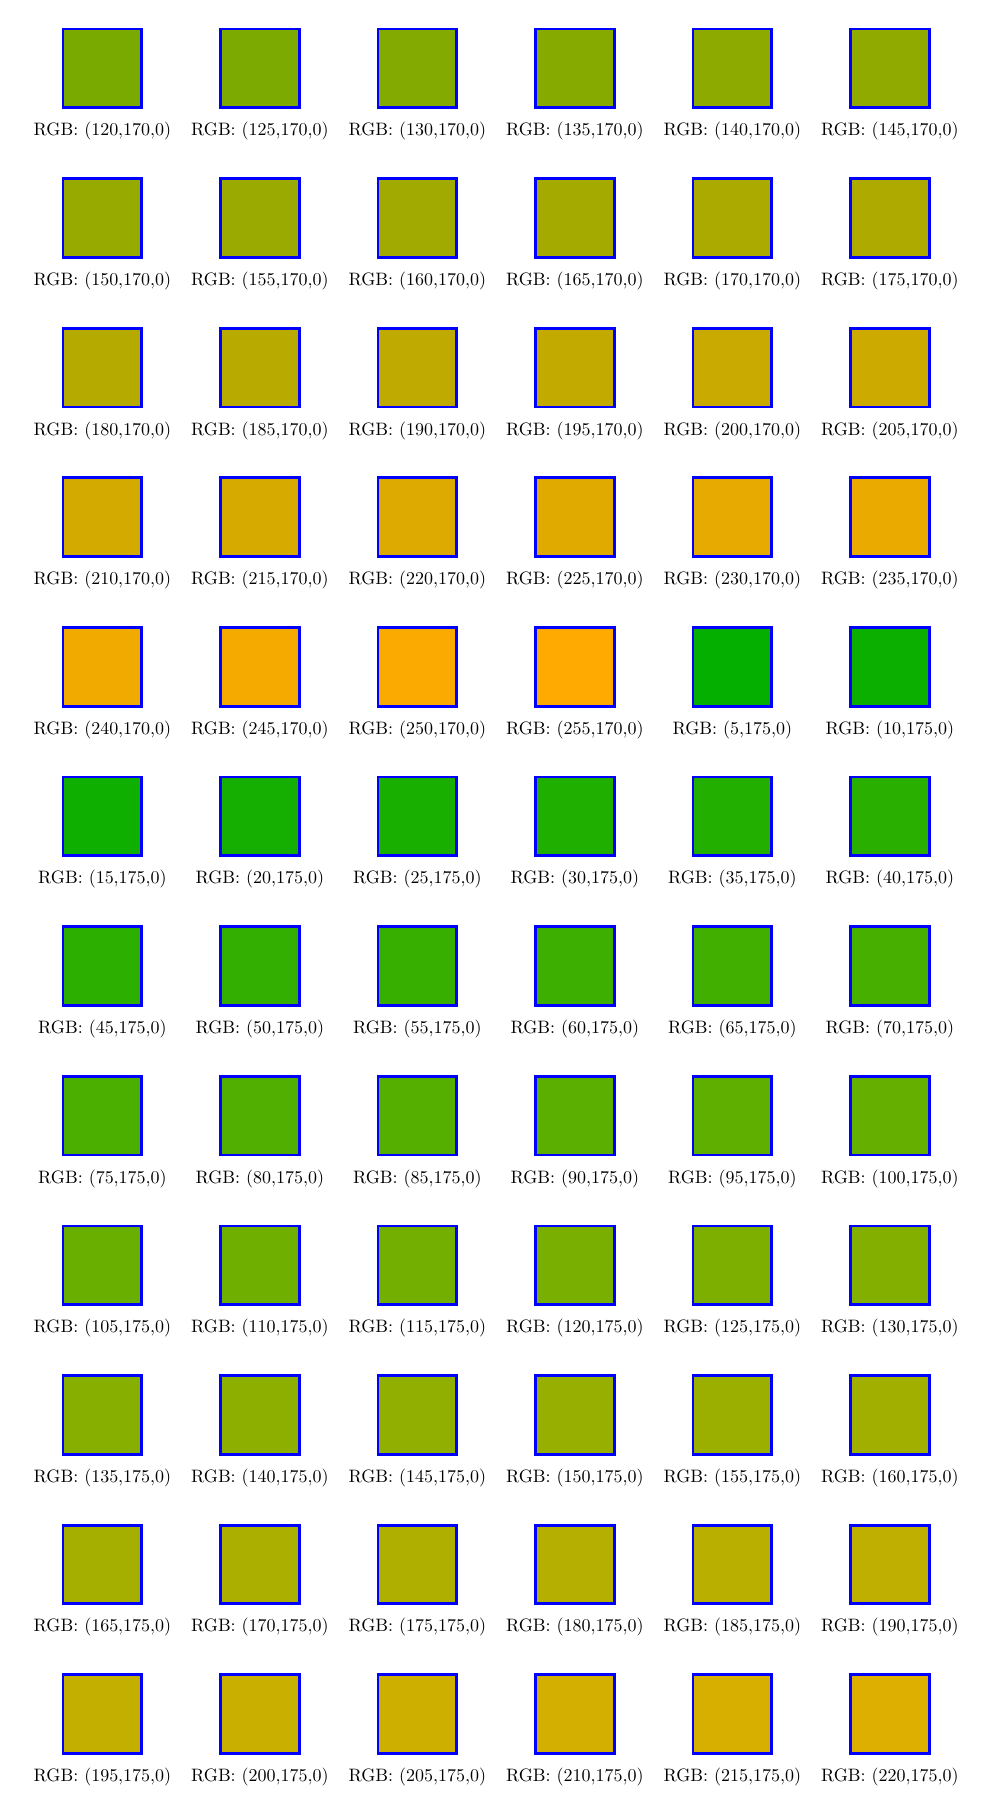
\begin{tikzpicture}

    \filldraw[draw=blue,line width=1,fill=colorR120G170B0]
    (0,0) rectangle (1,1);

    \node[scale=0.65] at (0.5,-0.3) {RGB: (120,170,0)};



    \begin{scope}[xshift=2cm]

      \filldraw[draw=blue,line width=1,fill=colorR125G170B0]
      (0,0) rectangle (1,1);

      \node[scale=0.65] at (0.5,-0.3) {RGB: (125,170,0)};

    \end{scope}



    \begin{scope}[xshift=4cm]

      \filldraw[draw=blue,line width=1,fill=colorR130G170B0]
      (0,0) rectangle (1,1);

      \node[scale=0.65] at (0.5,-0.3) {RGB: (130,170,0)};

    \end{scope}



    \begin{scope}[xshift=6cm]

      \filldraw[draw=blue,line width=1,fill=colorR135G170B0]
      (0,0) rectangle (1,1);

      \node[scale=0.65] at (0.5,-0.3) {RGB: (135,170,0)};

    \end{scope}



    \begin{scope}[xshift=8cm]

      \filldraw[draw=blue,line width=1,fill=colorR140G170B0]
      (0,0) rectangle (1,1);

      \node[scale=0.65] at (0.5,-0.3) {RGB: (140,170,0)};

    \end{scope}



    \begin{scope}[xshift=10cm]

      \filldraw[draw=blue,line width=1,fill=colorR145G170B0]
      (0,0) rectangle (1,1);

      \node[scale=0.65] at (0.5,-0.3) {RGB: (145,170,0)};

    \end{scope}







    \begin{scope}[yshift=-1.9cm]

      \filldraw[draw=blue,line width=1,fill=colorR150G170B0]
      (0,0) rectangle (1,1);

      \node[scale=0.65] at (0.5,-0.3) {RGB: (150,170,0)};

    \end{scope}



    \begin{scope}[xshift=2cm,yshift=-1.9cm]

      \filldraw[draw=blue,line width=1,fill=colorR155G170B0]
      (0,0) rectangle (1,1);

      \node[scale=0.65] at (0.5,-0.3) {RGB: (155,170,0)};

    \end{scope}



    \begin{scope}[xshift=4cm,yshift=-1.9cm]

      \filldraw[draw=blue,line width=1,fill=colorR160G170B0]
      (0,0) rectangle (1,1);

      \node[scale=0.65] at (0.5,-0.3) {RGB: (160,170,0)};

    \end{scope}



    \begin{scope}[xshift=6cm,yshift=-1.9cm]

      \filldraw[draw=blue,line width=1,fill=colorR165G170B0]
      (0,0) rectangle (1,1);

      \node[scale=0.65] at (0.5,-0.3) {RGB: (165,170,0)};

    \end{scope}



    \begin{scope}[xshift=8cm,yshift=-1.9cm]

      \filldraw[draw=blue,line width=1,fill=colorR170G170B0]
      (0,0) rectangle (1,1);

      \node[scale=0.65] at (0.5,-0.3) {RGB: (170,170,0)};

    \end{scope}



    \begin{scope}[xshift=10cm,yshift=-1.9cm]

      \filldraw[draw=blue,line width=1,fill=colorR175G170B0]
      (0,0) rectangle (1,1);

      \node[scale=0.65] at (0.5,-0.3) {RGB: (175,170,0)};

    \end{scope}







    \begin{scope}[yshift=-3.8cm]

      \filldraw[draw=blue,line width=1,fill=colorR180G170B0]
      (0,0) rectangle (1,1);

      \node[scale=0.65] at (0.5,-0.3) {RGB: (180,170,0)};

    \end{scope}



    \begin{scope}[xshift=2cm,yshift=-3.8cm]

      \filldraw[draw=blue,line width=1,fill=colorR185G170B0]
      (0,0) rectangle (1,1);

      \node[scale=0.65] at (0.5,-0.3) {RGB: (185,170,0)};

    \end{scope}



    \begin{scope}[xshift=4cm,yshift=-3.8cm]

      \filldraw[draw=blue,line width=1,fill=colorR190G170B0]
      (0,0) rectangle (1,1);

      \node[scale=0.65] at (0.5,-0.3) {RGB: (190,170,0)};

    \end{scope}



    \begin{scope}[xshift=6cm,yshift=-3.8cm]

      \filldraw[draw=blue,line width=1,fill=colorR195G170B0]
      (0,0) rectangle (1,1);

      \node[scale=0.65] at (0.5,-0.3) {RGB: (195,170,0)};

    \end{scope}



    \begin{scope}[xshift=8cm,yshift=-3.8cm]

      \filldraw[draw=blue,line width=1,fill=colorR200G170B0]
      (0,0) rectangle (1,1);

      \node[scale=0.65] at (0.5,-0.3) {RGB: (200,170,0)};

    \end{scope}



    \begin{scope}[xshift=10cm,yshift=-3.8cm]

      \filldraw[draw=blue,line width=1,fill=colorR205G170B0]
      (0,0) rectangle (1,1);

      \node[scale=0.65] at (0.5,-0.3) {RGB: (205,170,0)};

    \end{scope}







    \begin{scope}[yshift=-5.7cm]

      \filldraw[draw=blue,line width=1,fill=colorR210G170B0]
      (0,0) rectangle (1,1);

      \node[scale=0.65] at (0.5,-0.3) {RGB: (210,170,0)};

    \end{scope}



    \begin{scope}[xshift=2cm,yshift=-5.7cm]

      \filldraw[draw=blue,line width=1,fill=colorR215G170B0]
      (0,0) rectangle (1,1);

      \node[scale=0.65] at (0.5,-0.3) {RGB: (215,170,0)};

    \end{scope}



    \begin{scope}[xshift=4cm,yshift=-5.7cm]

      \filldraw[draw=blue,line width=1,fill=colorR220G170B0]
      (0,0) rectangle (1,1);

      \node[scale=0.65] at (0.5,-0.3) {RGB: (220,170,0)};

    \end{scope}



    \begin{scope}[xshift=6cm,yshift=-5.7cm]

      \filldraw[draw=blue,line width=1,fill=colorR225G170B0]
      (0,0) rectangle (1,1);

      \node[scale=0.65] at (0.5,-0.3) {RGB: (225,170,0)};

    \end{scope}



    \begin{scope}[xshift=8cm,yshift=-5.7cm]

      \filldraw[draw=blue,line width=1,fill=colorR230G170B0]
      (0,0) rectangle (1,1);

      \node[scale=0.65] at (0.5,-0.3) {RGB: (230,170,0)};

    \end{scope}



    \begin{scope}[xshift=10cm,yshift=-5.7cm]

      \filldraw[draw=blue,line width=1,fill=colorR235G170B0]
      (0,0) rectangle (1,1);

      \node[scale=0.65] at (0.5,-0.3) {RGB: (235,170,0)};

    \end{scope}







    \begin{scope}[yshift=-7.6cm]

      \filldraw[draw=blue,line width=1,fill=colorR240G170B0]
      (0,0) rectangle (1,1);

      \node[scale=0.65] at (0.5,-0.3) {RGB: (240,170,0)};

    \end{scope}



    \begin{scope}[xshift=2cm,yshift=-7.6cm]

      \filldraw[draw=blue,line width=1,fill=colorR245G170B0]
      (0,0) rectangle (1,1);

      \node[scale=0.65] at (0.5,-0.3) {RGB: (245,170,0)};

    \end{scope}



    \begin{scope}[xshift=4cm,yshift=-7.6cm]

      \filldraw[draw=blue,line width=1,fill=colorR250G170B0]
      (0,0) rectangle (1,1);

      \node[scale=0.65] at (0.5,-0.3) {RGB: (250,170,0)};

    \end{scope}



    \begin{scope}[xshift=6cm,yshift=-7.6cm]

      \filldraw[draw=blue,line width=1,fill=colorR255G170B0]
      (0,0) rectangle (1,1);

      \node[scale=0.65] at (0.5,-0.3) {RGB: (255,170,0)};

    \end{scope}



    \begin{scope}[xshift=8cm,yshift=-7.6cm]

      \filldraw[draw=blue,line width=1,fill=colorR5G175B0]
      (0,0) rectangle (1,1);

      \node[scale=0.65] at (0.5,-0.3) {RGB: (5,175,0)};

    \end{scope}



    \begin{scope}[xshift=10cm,yshift=-7.6cm]

      \filldraw[draw=blue,line width=1,fill=colorR10G175B0]
      (0,0) rectangle (1,1);

      \node[scale=0.65] at (0.5,-0.3) {RGB: (10,175,0)};

    \end{scope}







    \begin{scope}[yshift=-9.5cm]

      \filldraw[draw=blue,line width=1,fill=colorR15G175B0]
      (0,0) rectangle (1,1);

      \node[scale=0.65] at (0.5,-0.3) {RGB: (15,175,0)};

    \end{scope}



    \begin{scope}[xshift=2cm,yshift=-9.5cm]

      \filldraw[draw=blue,line width=1,fill=colorR20G175B0]
      (0,0) rectangle (1,1);

      \node[scale=0.65] at (0.5,-0.3) {RGB: (20,175,0)};

    \end{scope}



    \begin{scope}[xshift=4cm,yshift=-9.5cm]

      \filldraw[draw=blue,line width=1,fill=colorR25G175B0]
      (0,0) rectangle (1,1);

      \node[scale=0.65] at (0.5,-0.3) {RGB: (25,175,0)};

    \end{scope}



    \begin{scope}[xshift=6cm,yshift=-9.5cm]

      \filldraw[draw=blue,line width=1,fill=colorR30G175B0]
      (0,0) rectangle (1,1);

      \node[scale=0.65] at (0.5,-0.3) {RGB: (30,175,0)};

    \end{scope}



    \begin{scope}[xshift=8cm,yshift=-9.5cm]

      \filldraw[draw=blue,line width=1,fill=colorR35G175B0]
      (0,0) rectangle (1,1);

      \node[scale=0.65] at (0.5,-0.3) {RGB: (35,175,0)};

    \end{scope}



    \begin{scope}[xshift=10cm,yshift=-9.5cm]

      \filldraw[draw=blue,line width=1,fill=colorR40G175B0]
      (0,0) rectangle (1,1);

      \node[scale=0.65] at (0.5,-0.3) {RGB: (40,175,0)};

    \end{scope}







    \begin{scope}[yshift=-11.4cm]

      \filldraw[draw=blue,line width=1,fill=colorR45G175B0]
      (0,0) rectangle (1,1);

      \node[scale=0.65] at (0.5,-0.3) {RGB: (45,175,0)};

    \end{scope}



    \begin{scope}[xshift=2cm,yshift=-11.4cm]

      \filldraw[draw=blue,line width=1,fill=colorR50G175B0]
      (0,0) rectangle (1,1);

      \node[scale=0.65] at (0.5,-0.3) {RGB: (50,175,0)};

    \end{scope}



    \begin{scope}[xshift=4cm,yshift=-11.4cm]

      \filldraw[draw=blue,line width=1,fill=colorR55G175B0]
      (0,0) rectangle (1,1);

      \node[scale=0.65] at (0.5,-0.3) {RGB: (55,175,0)};

    \end{scope}



    \begin{scope}[xshift=6cm,yshift=-11.4cm]

      \filldraw[draw=blue,line width=1,fill=colorR60G175B0]
      (0,0) rectangle (1,1);

      \node[scale=0.65] at (0.5,-0.3) {RGB: (60,175,0)};

    \end{scope}



    \begin{scope}[xshift=8cm,yshift=-11.4cm]

      \filldraw[draw=blue,line width=1,fill=colorR65G175B0]
      (0,0) rectangle (1,1);

      \node[scale=0.65] at (0.5,-0.3) {RGB: (65,175,0)};

    \end{scope}



    \begin{scope}[xshift=10cm,yshift=-11.4cm]

      \filldraw[draw=blue,line width=1,fill=colorR70G175B0]
      (0,0) rectangle (1,1);

      \node[scale=0.65] at (0.5,-0.3) {RGB: (70,175,0)};

    \end{scope}







    \begin{scope}[yshift=-13.3cm]

      \filldraw[draw=blue,line width=1,fill=colorR75G175B0]
      (0,0) rectangle (1,1);

      \node[scale=0.65] at (0.5,-0.3) {RGB: (75,175,0)};

    \end{scope}



    \begin{scope}[xshift=2cm,yshift=-13.3cm]

      \filldraw[draw=blue,line width=1,fill=colorR80G175B0]
      (0,0) rectangle (1,1);

      \node[scale=0.65] at (0.5,-0.3) {RGB: (80,175,0)};

    \end{scope}



    \begin{scope}[xshift=4cm,yshift=-13.3cm]

      \filldraw[draw=blue,line width=1,fill=colorR85G175B0]
      (0,0) rectangle (1,1);

      \node[scale=0.65] at (0.5,-0.3) {RGB: (85,175,0)};

    \end{scope}



    \begin{scope}[xshift=6cm,yshift=-13.3cm]

      \filldraw[draw=blue,line width=1,fill=colorR90G175B0]
      (0,0) rectangle (1,1);

      \node[scale=0.65] at (0.5,-0.3) {RGB: (90,175,0)};

    \end{scope}



    \begin{scope}[xshift=8cm,yshift=-13.3cm]

      \filldraw[draw=blue,line width=1,fill=colorR95G175B0]
      (0,0) rectangle (1,1);

      \node[scale=0.65] at (0.5,-0.3) {RGB: (95,175,0)};

    \end{scope}



    \begin{scope}[xshift=10cm,yshift=-13.3cm]

      \filldraw[draw=blue,line width=1,fill=colorR100G175B0]
      (0,0) rectangle (1,1);

      \node[scale=0.65] at (0.5,-0.3) {RGB: (100,175,0)};

    \end{scope}







    \begin{scope}[yshift=-15.2cm]

      \filldraw[draw=blue,line width=1,fill=colorR105G175B0]
      (0,0) rectangle (1,1);

      \node[scale=0.65] at (0.5,-0.3) {RGB: (105,175,0)};

    \end{scope}



    \begin{scope}[xshift=2cm,yshift=-15.2cm]

      \filldraw[draw=blue,line width=1,fill=colorR110G175B0]
      (0,0) rectangle (1,1);

      \node[scale=0.65] at (0.5,-0.3) {RGB: (110,175,0)};

    \end{scope}



    \begin{scope}[xshift=4cm,yshift=-15.2cm]

      \filldraw[draw=blue,line width=1,fill=colorR115G175B0]
      (0,0) rectangle (1,1);

      \node[scale=0.65] at (0.5,-0.3) {RGB: (115,175,0)};

    \end{scope}



    \begin{scope}[xshift=6cm,yshift=-15.2cm]

      \filldraw[draw=blue,line width=1,fill=colorR120G175B0]
      (0,0) rectangle (1,1);

      \node[scale=0.65] at (0.5,-0.3) {RGB: (120,175,0)};

    \end{scope}



    \begin{scope}[xshift=8cm,yshift=-15.2cm]

      \filldraw[draw=blue,line width=1,fill=colorR125G175B0]
      (0,0) rectangle (1,1);

      \node[scale=0.65] at (0.5,-0.3) {RGB: (125,175,0)};

    \end{scope}



    \begin{scope}[xshift=10cm,yshift=-15.2cm]

      \filldraw[draw=blue,line width=1,fill=colorR130G175B0]
      (0,0) rectangle (1,1);

      \node[scale=0.65] at (0.5,-0.3) {RGB: (130,175,0)};

    \end{scope}







    \begin{scope}[yshift=-17.1cm]

      \filldraw[draw=blue,line width=1,fill=colorR135G175B0]
      (0,0) rectangle (1,1);

      \node[scale=0.65] at (0.5,-0.3) {RGB: (135,175,0)};

    \end{scope}



    \begin{scope}[xshift=2cm,yshift=-17.1cm]

      \filldraw[draw=blue,line width=1,fill=colorR140G175B0]
      (0,0) rectangle (1,1);

      \node[scale=0.65] at (0.5,-0.3) {RGB: (140,175,0)};

    \end{scope}



    \begin{scope}[xshift=4cm,yshift=-17.1cm]

      \filldraw[draw=blue,line width=1,fill=colorR145G175B0]
      (0,0) rectangle (1,1);

      \node[scale=0.65] at (0.5,-0.3) {RGB: (145,175,0)};

    \end{scope}



    \begin{scope}[xshift=6cm,yshift=-17.1cm]

      \filldraw[draw=blue,line width=1,fill=colorR150G175B0]
      (0,0) rectangle (1,1);

      \node[scale=0.65] at (0.5,-0.3) {RGB: (150,175,0)};

    \end{scope}



    \begin{scope}[xshift=8cm,yshift=-17.1cm]

      \filldraw[draw=blue,line width=1,fill=colorR155G175B0]
      (0,0) rectangle (1,1);

      \node[scale=0.65] at (0.5,-0.3) {RGB: (155,175,0)};

    \end{scope}



    \begin{scope}[xshift=10cm,yshift=-17.1cm]

      \filldraw[draw=blue,line width=1,fill=colorR160G175B0]
      (0,0) rectangle (1,1);

      \node[scale=0.65] at (0.5,-0.3) {RGB: (160,175,0)};

    \end{scope}







    \begin{scope}[yshift=-19cm]

      \filldraw[draw=blue,line width=1,fill=colorR165G175B0]
      (0,0) rectangle (1,1);

      \node[scale=0.65] at (0.5,-0.3) {RGB: (165,175,0)};

    \end{scope}



    \begin{scope}[xshift=2cm,yshift=-19cm]

      \filldraw[draw=blue,line width=1,fill=colorR170G175B0]
      (0,0) rectangle (1,1);

      \node[scale=0.65] at (0.5,-0.3) {RGB: (170,175,0)};

    \end{scope}



    \begin{scope}[xshift=4cm,yshift=-19cm]

      \filldraw[draw=blue,line width=1,fill=colorR175G175B0]
      (0,0) rectangle (1,1);

      \node[scale=0.65] at (0.5,-0.3) {RGB: (175,175,0)};

    \end{scope}



    \begin{scope}[xshift=6cm,yshift=-19cm]

      \filldraw[draw=blue,line width=1,fill=colorR180G175B0]
      (0,0) rectangle (1,1);

      \node[scale=0.65] at (0.5,-0.3) {RGB: (180,175,0)};

    \end{scope}



    \begin{scope}[xshift=8cm,yshift=-19cm]

      \filldraw[draw=blue,line width=1,fill=colorR185G175B0]
      (0,0) rectangle (1,1);

      \node[scale=0.65] at (0.5,-0.3) {RGB: (185,175,0)};

    \end{scope}



    \begin{scope}[xshift=10cm,yshift=-19cm]

      \filldraw[draw=blue,line width=1,fill=colorR190G175B0]
      (0,0) rectangle (1,1);

      \node[scale=0.65] at (0.5,-0.3) {RGB: (190,175,0)};

    \end{scope}







    \begin{scope}[yshift=-20.9cm]

      \filldraw[draw=blue,line width=1,fill=colorR195G175B0]
      (0,0) rectangle (1,1);

      \node[scale=0.65] at (0.5,-0.3) {RGB: (195,175,0)};

    \end{scope}



    \begin{scope}[xshift=2cm,yshift=-20.9cm]

      \filldraw[draw=blue,line width=1,fill=colorR200G175B0]
      (0,0) rectangle (1,1);

      \node[scale=0.65] at (0.5,-0.3) {RGB: (200,175,0)};

    \end{scope}



    \begin{scope}[xshift=4cm,yshift=-20.9cm]

      \filldraw[draw=blue,line width=1,fill=colorR205G175B0]
      (0,0) rectangle (1,1);

      \node[scale=0.65] at (0.5,-0.3) {RGB: (205,175,0)};

    \end{scope}



    \begin{scope}[xshift=6cm,yshift=-20.9cm]

      \filldraw[draw=blue,line width=1,fill=colorR210G175B0]
      (0,0) rectangle (1,1);

      \node[scale=0.65] at (0.5,-0.3) {RGB: (210,175,0)};

    \end{scope}



    \begin{scope}[xshift=8cm,yshift=-20.9cm]

      \filldraw[draw=blue,line width=1,fill=colorR215G175B0]
      (0,0) rectangle (1,1);

      \node[scale=0.65] at (0.5,-0.3) {RGB: (215,175,0)};

    \end{scope}



    \begin{scope}[xshift=10cm,yshift=-20.9cm]

      \filldraw[draw=blue,line width=1,fill=colorR220G175B0]
      (0,0) rectangle (1,1);

      \node[scale=0.65] at (0.5,-0.3) {RGB: (220,175,0)};

    \end{scope}

  \end{tikzpicture}

  \caption{Mixed colors in~RGB system: $(120,170,0)$--$(255,170,0)$,
    $(5,175,0)$--$(220,175,0)$}



  \label{fig:Mixed-colors-Part-07}

\end{figure}
% ##################





% ##################
\begin{figure}

  \centering


  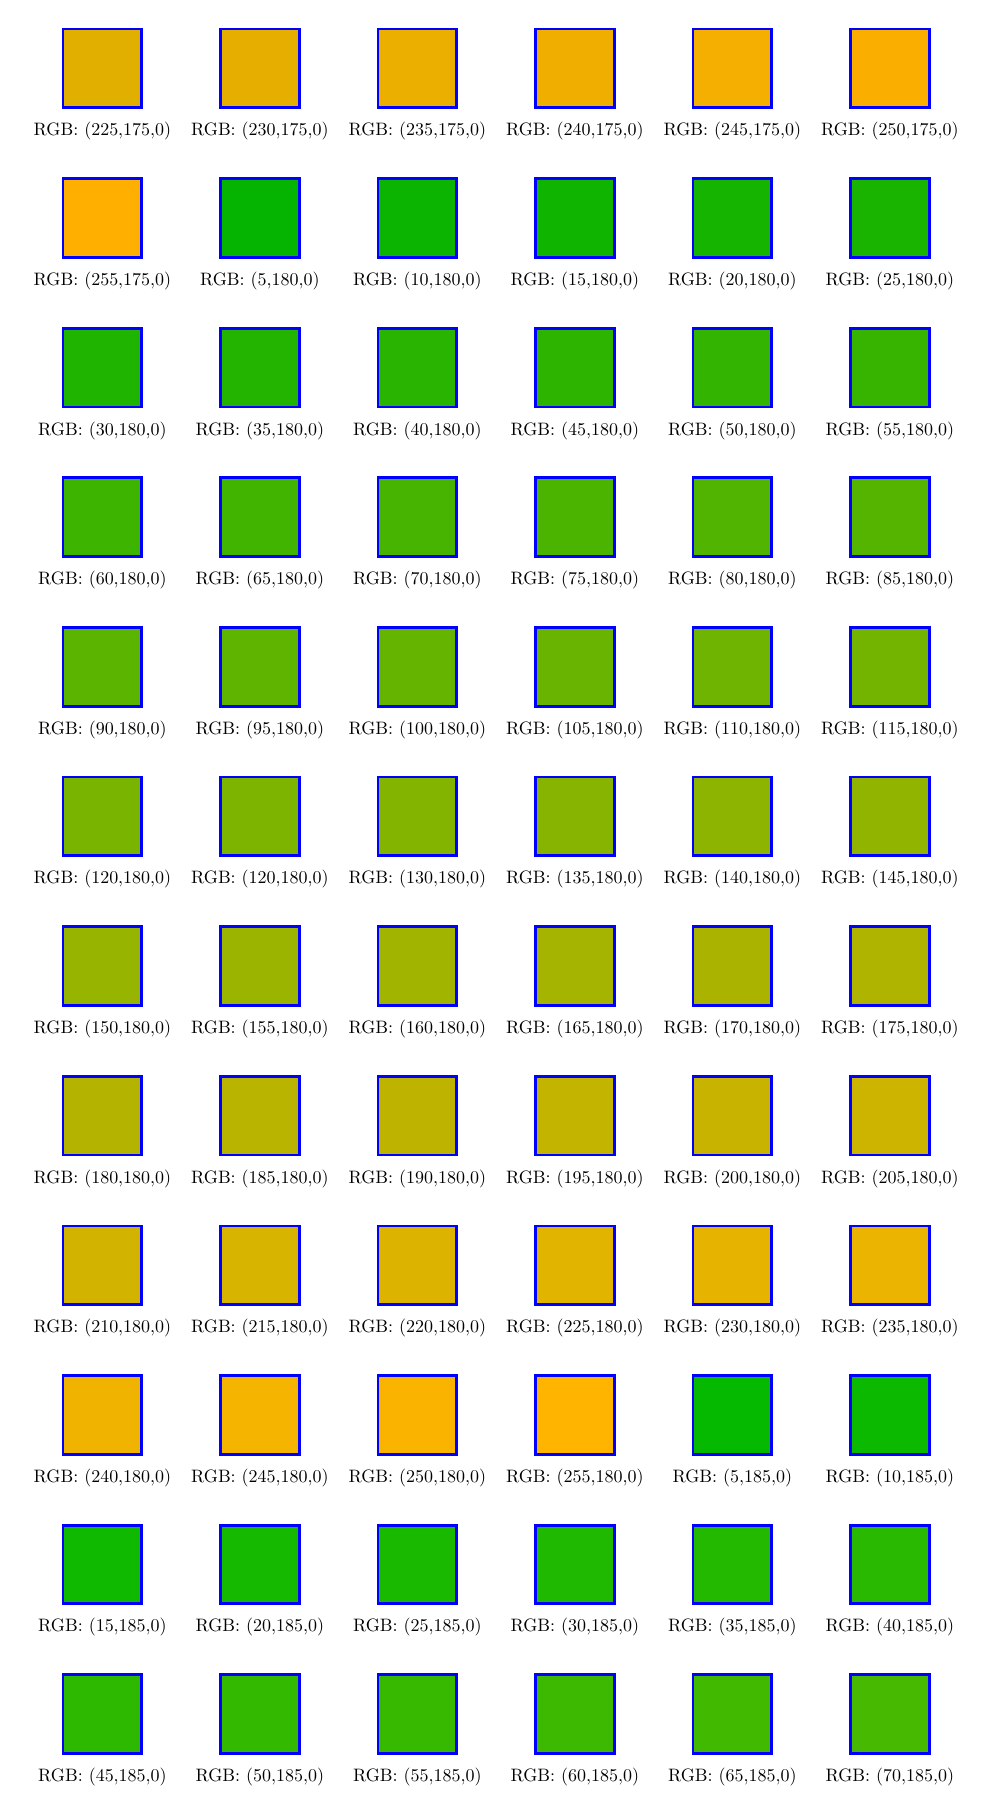
\begin{tikzpicture}

    \filldraw[draw=blue,line width=1,fill=colorR225G175B0]
    (0,0) rectangle (1,1);

    \node[scale=0.65] at (0.5,-0.3) {RGB: (225,175,0)};



    \begin{scope}[xshift=2cm]

      \filldraw[draw=blue,line width=1,fill=colorR230G175B0]
      (0,0) rectangle (1,1);

      \node[scale=0.65] at (0.5,-0.3) {RGB: (230,175,0)};

    \end{scope}



    \begin{scope}[xshift=4cm]

      \filldraw[draw=blue,line width=1,fill=colorR235G175B0]
      (0,0) rectangle (1,1);

      \node[scale=0.65] at (0.5,-0.3) {RGB: (235,175,0)};

    \end{scope}



    \begin{scope}[xshift=6cm]

      \filldraw[draw=blue,line width=1,fill=colorR240G175B0]
      (0,0) rectangle (1,1);

      \node[scale=0.65] at (0.5,-0.3) {RGB: (240,175,0)};

    \end{scope}



    \begin{scope}[xshift=8cm]

      \filldraw[draw=blue,line width=1,fill=colorR245G175B0]
      (0,0) rectangle (1,1);

      \node[scale=0.65] at (0.5,-0.3) {RGB: (245,175,0)};

    \end{scope}



    \begin{scope}[xshift=10cm]

      \filldraw[draw=blue,line width=1,fill=colorR250G175B0]
      (0,0) rectangle (1,1);

      \node[scale=0.65] at (0.5,-0.3) {RGB: (250,175,0)};

    \end{scope}







    \begin{scope}[yshift=-1.9cm]

      \filldraw[draw=blue,line width=1,fill=colorR255G175B0]
      (0,0) rectangle (1,1);

      \node[scale=0.65] at (0.5,-0.3) {RGB: (255,175,0)};

    \end{scope}



    \begin{scope}[xshift=2cm,yshift=-1.9cm]

      \filldraw[draw=blue,line width=1,fill=colorR5G180B0]
      (0,0) rectangle (1,1);

      \node[scale=0.65] at (0.5,-0.3) {RGB: (5,180,0)};

    \end{scope}



    \begin{scope}[xshift=4cm,yshift=-1.9cm]

      \filldraw[draw=blue,line width=1,fill=colorR10G180B0]
      (0,0) rectangle (1,1);

      \node[scale=0.65] at (0.5,-0.3) {RGB: (10,180,0)};

    \end{scope}



    \begin{scope}[xshift=6cm,yshift=-1.9cm]

      \filldraw[draw=blue,line width=1,fill=colorR15G180B0]
      (0,0) rectangle (1,1);

      \node[scale=0.65] at (0.5,-0.3) {RGB: (15,180,0)};

    \end{scope}



    \begin{scope}[xshift=8cm,yshift=-1.9cm]

      \filldraw[draw=blue,line width=1,fill=colorR20G180B0]
      (0,0) rectangle (1,1);

      \node[scale=0.65] at (0.5,-0.3) {RGB: (20,180,0)};

    \end{scope}



    \begin{scope}[xshift=10cm,yshift=-1.9cm]

      \filldraw[draw=blue,line width=1,fill=colorR25G180B0]
      (0,0) rectangle (1,1);

      \node[scale=0.65] at (0.5,-0.3) {RGB: (25,180,0)};

    \end{scope}







    \begin{scope}[yshift=-3.8cm]

      \filldraw[draw=blue,line width=1,fill=colorR30G180B0]
      (0,0) rectangle (1,1);

      \node[scale=0.65] at (0.5,-0.3) {RGB: (30,180,0)};

    \end{scope}



    \begin{scope}[xshift=2cm,yshift=-3.8cm]

      \filldraw[draw=blue,line width=1,fill=colorR35G180B0]
      (0,0) rectangle (1,1);

      \node[scale=0.65] at (0.5,-0.3) {RGB: (35,180,0)};

    \end{scope}



    \begin{scope}[xshift=4cm,yshift=-3.8cm]

      \filldraw[draw=blue,line width=1,fill=colorR40G180B0]
      (0,0) rectangle (1,1);

      \node[scale=0.65] at (0.5,-0.3) {RGB: (40,180,0)};

    \end{scope}



    \begin{scope}[xshift=6cm,yshift=-3.8cm]

      \filldraw[draw=blue,line width=1,fill=colorR45G180B0]
      (0,0) rectangle (1,1);

      \node[scale=0.65] at (0.5,-0.3) {RGB: (45,180,0)};

    \end{scope}



    \begin{scope}[xshift=8cm,yshift=-3.8cm]

      \filldraw[draw=blue,line width=1,fill=colorR50G180B0]
      (0,0) rectangle (1,1);

      \node[scale=0.65] at (0.5,-0.3) {RGB: (50,180,0)};

    \end{scope}



    \begin{scope}[xshift=10cm,yshift=-3.8cm]

      \filldraw[draw=blue,line width=1,fill=colorR55G180B0]
      (0,0) rectangle (1,1);

      \node[scale=0.65] at (0.5,-0.3) {RGB: (55,180,0)};

    \end{scope}







    \begin{scope}[yshift=-5.7cm]

      \filldraw[draw=blue,line width=1,fill=colorR60G180B0]
      (0,0) rectangle (1,1);

      \node[scale=0.65] at (0.5,-0.3) {RGB: (60,180,0)};

    \end{scope}



    \begin{scope}[xshift=2cm,yshift=-5.7cm]

      \filldraw[draw=blue,line width=1,fill=colorR65G180B0]
      (0,0) rectangle (1,1);

      \node[scale=0.65] at (0.5,-0.3) {RGB: (65,180,0)};

    \end{scope}



    \begin{scope}[xshift=4cm,yshift=-5.7cm]

      \filldraw[draw=blue,line width=1,fill=colorR70G180B0]
      (0,0) rectangle (1,1);

      \node[scale=0.65] at (0.5,-0.3) {RGB: (70,180,0)};

    \end{scope}



    \begin{scope}[xshift=6cm,yshift=-5.7cm]

      \filldraw[draw=blue,line width=1,fill=colorR75G180B0]
      (0,0) rectangle (1,1);

      \node[scale=0.65] at (0.5,-0.3) {RGB: (75,180,0)};

    \end{scope}



    \begin{scope}[xshift=8cm,yshift=-5.7cm]

      \filldraw[draw=blue,line width=1,fill=colorR80G180B0]
      (0,0) rectangle (1,1);

      \node[scale=0.65] at (0.5,-0.3) {RGB: (80,180,0)};

    \end{scope}



    \begin{scope}[xshift=10cm,yshift=-5.7cm]

      \filldraw[draw=blue,line width=1,fill=colorR85G180B0]
      (0,0) rectangle (1,1);

      \node[scale=0.65] at (0.5,-0.3) {RGB: (85,180,0)};

    \end{scope}







    \begin{scope}[yshift=-7.6cm]

      \filldraw[draw=blue,line width=1,fill=colorR90G180B0]
      (0,0) rectangle (1,1);

      \node[scale=0.65] at (0.5,-0.3) {RGB: (90,180,0)};

    \end{scope}



    \begin{scope}[xshift=2cm,yshift=-7.6cm]

      \filldraw[draw=blue,line width=1,fill=colorR95G180B0]
      (0,0) rectangle (1,1);

      \node[scale=0.65] at (0.5,-0.3) {RGB: (95,180,0)};

    \end{scope}



    \begin{scope}[xshift=4cm,yshift=-7.6cm]

      \filldraw[draw=blue,line width=1,fill=colorR100G180B0]
      (0,0) rectangle (1,1);

      \node[scale=0.65] at (0.5,-0.3) {RGB: (100,180,0)};

    \end{scope}



    \begin{scope}[xshift=6cm,yshift=-7.6cm]

      \filldraw[draw=blue,line width=1,fill=colorR105G180B0]
      (0,0) rectangle (1,1);

      \node[scale=0.65] at (0.5,-0.3) {RGB: (105,180,0)};

    \end{scope}



    \begin{scope}[xshift=8cm,yshift=-7.6cm]

      \filldraw[draw=blue,line width=1,fill=colorR110G180B0]
      (0,0) rectangle (1,1);

      \node[scale=0.65] at (0.5,-0.3) {RGB: (110,180,0)};

    \end{scope}



    \begin{scope}[xshift=10cm,yshift=-7.6cm]

      \filldraw[draw=blue,line width=1,fill=colorR115G180B0]
      (0,0) rectangle (1,1);

      \node[scale=0.65] at (0.5,-0.3) {RGB: (115,180,0)};

    \end{scope}







    \begin{scope}[yshift=-9.5cm]

      \filldraw[draw=blue,line width=1,fill=colorR120G180B0]
      (0,0) rectangle (1,1);

      \node[scale=0.65] at (0.5,-0.3) {RGB: (120,180,0)};

    \end{scope}



    \begin{scope}[xshift=2cm,yshift=-9.5cm]

      \filldraw[draw=blue,line width=1,fill=colorR125G180B0]
      (0,0) rectangle (1,1);

      \node[scale=0.65] at (0.5,-0.3) {RGB: (120,180,0)};

    \end{scope}



    \begin{scope}[xshift=4cm,yshift=-9.5cm]

      \filldraw[draw=blue,line width=1,fill=colorR130G180B0]
      (0,0) rectangle (1,1);

      \node[scale=0.65] at (0.5,-0.3) {RGB: (130,180,0)};

    \end{scope}



    \begin{scope}[xshift=6cm,yshift=-9.5cm]

      \filldraw[draw=blue,line width=1,fill=colorR135G180B0]
      (0,0) rectangle (1,1);

      \node[scale=0.65] at (0.5,-0.3) {RGB: (135,180,0)};

    \end{scope}



    \begin{scope}[xshift=8cm,yshift=-9.5cm]

      \filldraw[draw=blue,line width=1,fill=colorR140G180B0]
      (0,0) rectangle (1,1);

      \node[scale=0.65] at (0.5,-0.3) {RGB: (140,180,0)};

    \end{scope}



    \begin{scope}[xshift=10cm,yshift=-9.5cm]

      \filldraw[draw=blue,line width=1,fill=colorR145G180B0]
      (0,0) rectangle (1,1);

      \node[scale=0.65] at (0.5,-0.3) {RGB: (145,180,0)};

    \end{scope}







    \begin{scope}[yshift=-11.4cm]

      \filldraw[draw=blue,line width=1,fill=colorR150G180B0]
      (0,0) rectangle (1,1);

      \node[scale=0.65] at (0.5,-0.3) {RGB: (150,180,0)};

    \end{scope}



    \begin{scope}[xshift=2cm,yshift=-11.4cm]

      \filldraw[draw=blue,line width=1,fill=colorR155G180B0]
      (0,0) rectangle (1,1);

      \node[scale=0.65] at (0.5,-0.3) {RGB: (155,180,0)};

    \end{scope}



    \begin{scope}[xshift=4cm,yshift=-11.4cm]

      \filldraw[draw=blue,line width=1,fill=colorR160G180B0]
      (0,0) rectangle (1,1);

      \node[scale=0.65] at (0.5,-0.3) {RGB: (160,180,0)};

    \end{scope}



    \begin{scope}[xshift=6cm,yshift=-11.4cm]

      \filldraw[draw=blue,line width=1,fill=colorR165G180B0]
      (0,0) rectangle (1,1);

      \node[scale=0.65] at (0.5,-0.3) {RGB: (165,180,0)};

    \end{scope}



    \begin{scope}[xshift=8cm,yshift=-11.4cm]

      \filldraw[draw=blue,line width=1,fill=colorR170G180B0]
      (0,0) rectangle (1,1);

      \node[scale=0.65] at (0.5,-0.3) {RGB: (170,180,0)};

    \end{scope}



    \begin{scope}[xshift=10cm,yshift=-11.4cm]

      \filldraw[draw=blue,line width=1,fill=colorR175G180B0]
      (0,0) rectangle (1,1);

      \node[scale=0.65] at (0.5,-0.3) {RGB: (175,180,0)};

    \end{scope}







    \begin{scope}[yshift=-13.3cm]

      \filldraw[draw=blue,line width=1,fill=colorR180G180B0]
      (0,0) rectangle (1,1);

      \node[scale=0.65] at (0.5,-0.3) {RGB: (180,180,0)};

    \end{scope}



    \begin{scope}[xshift=2cm,yshift=-13.3cm]

      \filldraw[draw=blue,line width=1,fill=colorR185G180B0]
      (0,0) rectangle (1,1);

      \node[scale=0.65] at (0.5,-0.3) {RGB: (185,180,0)};

    \end{scope}



    \begin{scope}[xshift=4cm,yshift=-13.3cm]

      \filldraw[draw=blue,line width=1,fill=colorR190G180B0]
      (0,0) rectangle (1,1);

      \node[scale=0.65] at (0.5,-0.3) {RGB: (190,180,0)};

    \end{scope}



    \begin{scope}[xshift=6cm,yshift=-13.3cm]

      \filldraw[draw=blue,line width=1,fill=colorR195G180B0]
      (0,0) rectangle (1,1);

      \node[scale=0.65] at (0.5,-0.3) {RGB: (195,180,0)};

    \end{scope}



    \begin{scope}[xshift=8cm,yshift=-13.3cm]

      \filldraw[draw=blue,line width=1,fill=colorR200G180B0]
      (0,0) rectangle (1,1);

      \node[scale=0.65] at (0.5,-0.3) {RGB: (200,180,0)};

    \end{scope}



    \begin{scope}[xshift=10cm,yshift=-13.3cm]

      \filldraw[draw=blue,line width=1,fill=colorR205G180B0]
      (0,0) rectangle (1,1);

      \node[scale=0.65] at (0.5,-0.3) {RGB: (205,180,0)};

    \end{scope}







    \begin{scope}[yshift=-15.2cm]

      \filldraw[draw=blue,line width=1,fill=colorR210G180B0]
      (0,0) rectangle (1,1);

      \node[scale=0.65] at (0.5,-0.3) {RGB: (210,180,0)};

    \end{scope}



    \begin{scope}[xshift=2cm,yshift=-15.2cm]

      \filldraw[draw=blue,line width=1,fill=colorR215G180B0]
      (0,0) rectangle (1,1);

      \node[scale=0.65] at (0.5,-0.3) {RGB: (215,180,0)};

    \end{scope}



    \begin{scope}[xshift=4cm,yshift=-15.2cm]

      \filldraw[draw=blue,line width=1,fill=colorR220G180B0]
      (0,0) rectangle (1,1);

      \node[scale=0.65] at (0.5,-0.3) {RGB: (220,180,0)};

    \end{scope}



    \begin{scope}[xshift=6cm,yshift=-15.2cm]

      \filldraw[draw=blue,line width=1,fill=colorR225G180B0]
      (0,0) rectangle (1,1);

      \node[scale=0.65] at (0.5,-0.3) {RGB: (225,180,0)};

    \end{scope}



    \begin{scope}[xshift=8cm,yshift=-15.2cm]

      \filldraw[draw=blue,line width=1,fill=colorR230G180B0]
      (0,0) rectangle (1,1);

      \node[scale=0.65] at (0.5,-0.3) {RGB: (230,180,0)};

    \end{scope}



    \begin{scope}[xshift=10cm,yshift=-15.2cm]

      \filldraw[draw=blue,line width=1,fill=colorR235G180B0]
      (0,0) rectangle (1,1);

      \node[scale=0.65] at (0.5,-0.3) {RGB: (235,180,0)};

    \end{scope}







    \begin{scope}[yshift=-17.1cm]

      \filldraw[draw=blue,line width=1,fill=colorR240G180B0]
      (0,0) rectangle (1,1);

      \node[scale=0.65] at (0.5,-0.3) {RGB: (240,180,0)};

    \end{scope}



    \begin{scope}[xshift=2cm,yshift=-17.1cm]

      \filldraw[draw=blue,line width=1,fill=colorR245G180B0]
      (0,0) rectangle (1,1);

      \node[scale=0.65] at (0.5,-0.3) {RGB: (245,180,0)};

    \end{scope}



    \begin{scope}[xshift=4cm,yshift=-17.1cm]

      \filldraw[draw=blue,line width=1,fill=colorR250G180B0]
      (0,0) rectangle (1,1);

      \node[scale=0.65] at (0.5,-0.3) {RGB: (250,180,0)};

    \end{scope}



    \begin{scope}[xshift=6cm,yshift=-17.1cm]

      \filldraw[draw=blue,line width=1,fill=colorR255G180B0]
      (0,0) rectangle (1,1);

      \node[scale=0.65] at (0.5,-0.3) {RGB: (255,180,0)};

    \end{scope}



    \begin{scope}[xshift=8cm,yshift=-17.1cm]

      \filldraw[draw=blue,line width=1,fill=colorR5G185B0]
      (0,0) rectangle (1,1);

      \node[scale=0.65] at (0.5,-0.3) {RGB: (5,185,0)};

    \end{scope}



    \begin{scope}[xshift=10cm,yshift=-17.1cm]

      \filldraw[draw=blue,line width=1,fill=colorR10G185B0]
      (0,0) rectangle (1,1);

      \node[scale=0.65] at (0.5,-0.3) {RGB: (10,185,0)};

    \end{scope}







    \begin{scope}[yshift=-19cm]

      \filldraw[draw=blue,line width=1,fill=colorR15G185B0]
      (0,0) rectangle (1,1);

      \node[scale=0.65] at (0.5,-0.3) {RGB: (15,185,0)};

    \end{scope}



    \begin{scope}[xshift=2cm,yshift=-19cm]

      \filldraw[draw=blue,line width=1,fill=colorR20G185B0]
      (0,0) rectangle (1,1);

      \node[scale=0.65] at (0.5,-0.3) {RGB: (20,185,0)};

    \end{scope}



    \begin{scope}[xshift=4cm,yshift=-19cm]

      \filldraw[draw=blue,line width=1,fill=colorR25G185B0]
      (0,0) rectangle (1,1);

      \node[scale=0.65] at (0.5,-0.3) {RGB: (25,185,0)};

    \end{scope}



    \begin{scope}[xshift=6cm,yshift=-19cm]

      \filldraw[draw=blue,line width=1,fill=colorR30G185B0]
      (0,0) rectangle (1,1);

      \node[scale=0.65] at (0.5,-0.3) {RGB: (30,185,0)};

    \end{scope}



    \begin{scope}[xshift=8cm,yshift=-19cm]

      \filldraw[draw=blue,line width=1,fill=colorR35G185B0]
      (0,0) rectangle (1,1);

      \node[scale=0.65] at (0.5,-0.3) {RGB: (35,185,0)};

    \end{scope}



    \begin{scope}[xshift=10cm,yshift=-19cm]

      \filldraw[draw=blue,line width=1,fill=colorR40G185B0]
      (0,0) rectangle (1,1);

      \node[scale=0.65] at (0.5,-0.3) {RGB: (40,185,0)};

    \end{scope}







    \begin{scope}[yshift=-20.9cm]

      \filldraw[draw=blue,line width=1,fill=colorR45G185B0]
      (0,0) rectangle (1,1);

      \node[scale=0.65] at (0.5,-0.3) {RGB: (45,185,0)};

    \end{scope}



    \begin{scope}[xshift=2cm,yshift=-20.9cm]

      \filldraw[draw=blue,line width=1,fill=colorR50G185B0]
      (0,0) rectangle (1,1);

      \node[scale=0.65] at (0.5,-0.3) {RGB: (50,185,0)};

    \end{scope}



    \begin{scope}[xshift=4cm,yshift=-20.9cm]

      \filldraw[draw=blue,line width=1,fill=colorR55G185B0]
      (0,0) rectangle (1,1);

      \node[scale=0.65] at (0.5,-0.3) {RGB: (55,185,0)};

    \end{scope}



    \begin{scope}[xshift=6cm,yshift=-20.9cm]

      \filldraw[draw=blue,line width=1,fill=colorR60G185B0]
      (0,0) rectangle (1,1);

      \node[scale=0.65] at (0.5,-0.3) {RGB: (60,185,0)};

    \end{scope}



    \begin{scope}[xshift=8cm,yshift=-20.9cm]

      \filldraw[draw=blue,line width=1,fill=colorR65G185B0]
      (0,0) rectangle (1,1);

      \node[scale=0.65] at (0.5,-0.3) {RGB: (65,185,0)};

    \end{scope}



    \begin{scope}[xshift=10cm,yshift=-20.9cm]

      \filldraw[draw=blue,line width=1,fill=colorR70G185B0]
      (0,0) rectangle (1,1);

      \node[scale=0.65] at (0.5,-0.3) {RGB: (70,185,0)};

    \end{scope}

  \end{tikzpicture}

  \caption{Mixed colors in~RGB system: $(225,175,0)$--$(255,175,0)$,
    $(5,180,0)$--$(255,180,0)$, $(5,185,0)$--$(70,185,0)$}



  \label{fig:Mixed-colors-Part-08}

\end{figure}
% ##################





% ##################
\begin{figure}

  \centering


  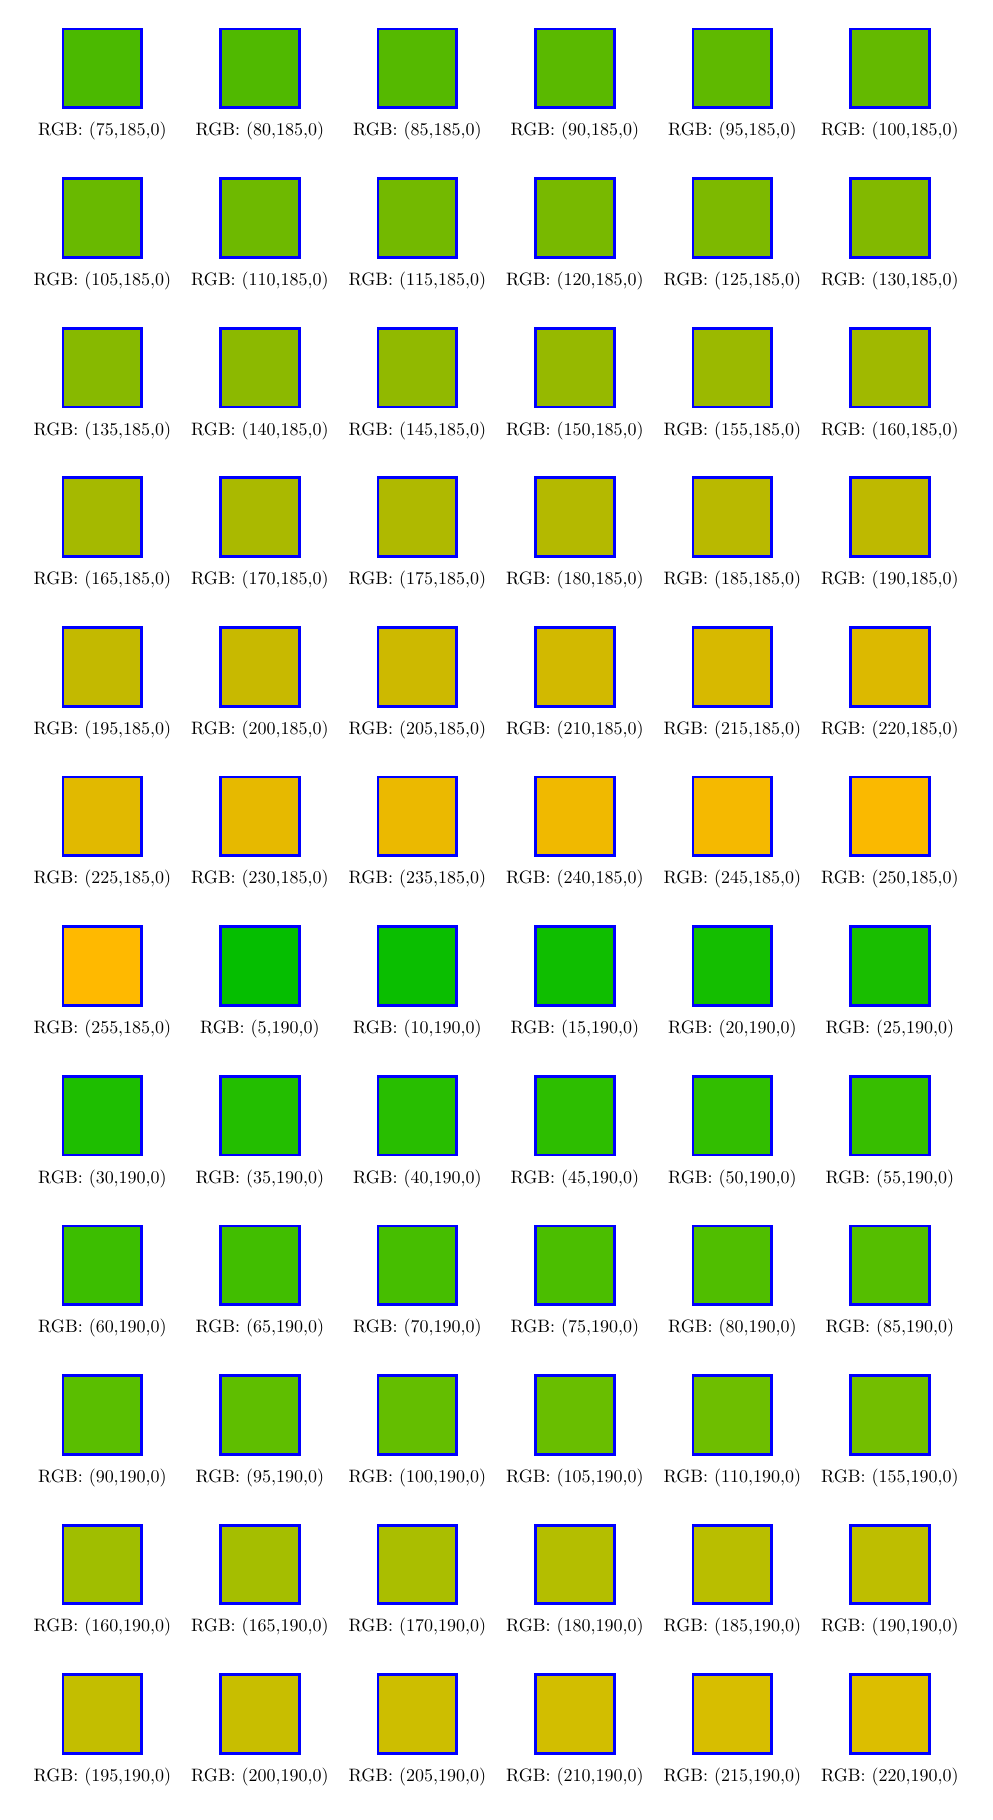
\begin{tikzpicture}

    \filldraw[draw=blue,line width=1,fill=colorR75G185B0]
    (0,0) rectangle (1,1);

    \node[scale=0.65] at (0.5,-0.3) {RGB: (75,185,0)};



    \begin{scope}[xshift=2cm]

      \filldraw[draw=blue,line width=1,fill=colorR80G185B0]
      (0,0) rectangle (1,1);

      \node[scale=0.65] at (0.5,-0.3) {RGB: (80,185,0)};

    \end{scope}



    \begin{scope}[xshift=4cm]

      \filldraw[draw=blue,line width=1,fill=colorR85G185B0]
      (0,0) rectangle (1,1);

      \node[scale=0.65] at (0.5,-0.3) {RGB: (85,185,0)};

    \end{scope}



    \begin{scope}[xshift=6cm]

      \filldraw[draw=blue,line width=1,fill=colorR90G185B0]
      (0,0) rectangle (1,1);

      \node[scale=0.65] at (0.5,-0.3) {RGB: (90,185,0)};

    \end{scope}



    \begin{scope}[xshift=8cm]

      \filldraw[draw=blue,line width=1,fill=colorR95G185B0]
      (0,0) rectangle (1,1);

      \node[scale=0.65] at (0.5,-0.3) {RGB: (95,185,0)};

    \end{scope}



    \begin{scope}[xshift=10cm]

      \filldraw[draw=blue,line width=1,fill=colorR100G185B0]
      (0,0) rectangle (1,1);

      \node[scale=0.65] at (0.5,-0.3) {RGB: (100,185,0)};

    \end{scope}







    \begin{scope}[yshift=-1.9cm]

      \filldraw[draw=blue,line width=1,fill=colorR105G185B0]
      (0,0) rectangle (1,1);

      \node[scale=0.65] at (0.5,-0.3) {RGB: (105,185,0)};

    \end{scope}



    \begin{scope}[xshift=2cm,yshift=-1.9cm]

      \filldraw[draw=blue,line width=1,fill=colorR110G185B0]
      (0,0) rectangle (1,1);

      \node[scale=0.65] at (0.5,-0.3) {RGB: (110,185,0)};

    \end{scope}



    \begin{scope}[xshift=4cm,yshift=-1.9cm]

      \filldraw[draw=blue,line width=1,fill=colorR115G185B0]
      (0,0) rectangle (1,1);

      \node[scale=0.65] at (0.5,-0.3) {RGB: (115,185,0)};

    \end{scope}



    \begin{scope}[xshift=6cm,yshift=-1.9cm]

      \filldraw[draw=blue,line width=1,fill=colorR120G185B0]
      (0,0) rectangle (1,1);

      \node[scale=0.65] at (0.5,-0.3) {RGB: (120,185,0)};

    \end{scope}



    \begin{scope}[xshift=8cm,yshift=-1.9cm]

      \filldraw[draw=blue,line width=1,fill=colorR125G185B0]
      (0,0) rectangle (1,1);

      \node[scale=0.65] at (0.5,-0.3) {RGB: (125,185,0)};

    \end{scope}



    \begin{scope}[xshift=10cm,yshift=-1.9cm]

      \filldraw[draw=blue,line width=1,fill=colorR130G185B0]
      (0,0) rectangle (1,1);

      \node[scale=0.65] at (0.5,-0.3) {RGB: (130,185,0)};

    \end{scope}







    \begin{scope}[yshift=-3.8cm]

      \filldraw[draw=blue,line width=1,fill=colorR135G185B0]
      (0,0) rectangle (1,1);

      \node[scale=0.65] at (0.5,-0.3) {RGB: (135,185,0)};

    \end{scope}



    \begin{scope}[xshift=2cm,yshift=-3.8cm]

      \filldraw[draw=blue,line width=1,fill=colorR140G185B0]
      (0,0) rectangle (1,1);

      \node[scale=0.65] at (0.5,-0.3) {RGB: (140,185,0)};

    \end{scope}



    \begin{scope}[xshift=4cm,yshift=-3.8cm]

      \filldraw[draw=blue,line width=1,fill=colorR145G185B0]
      (0,0) rectangle (1,1);

      \node[scale=0.65] at (0.5,-0.3) {RGB: (145,185,0)};

    \end{scope}



    \begin{scope}[xshift=6cm,yshift=-3.8cm]

      \filldraw[draw=blue,line width=1,fill=colorR150G185B0]
      (0,0) rectangle (1,1);

      \node[scale=0.65] at (0.5,-0.3) {RGB: (150,185,0)};

    \end{scope}



    \begin{scope}[xshift=8cm,yshift=-3.8cm]

      \filldraw[draw=blue,line width=1,fill=colorR155G185B0]
      (0,0) rectangle (1,1);

      \node[scale=0.65] at (0.5,-0.3) {RGB: (155,185,0)};

    \end{scope}



    \begin{scope}[xshift=10cm,yshift=-3.8cm]

      \filldraw[draw=blue,line width=1,fill=colorR160G185B0]
      (0,0) rectangle (1,1);

      \node[scale=0.65] at (0.5,-0.3) {RGB: (160,185,0)};

    \end{scope}







    \begin{scope}[yshift=-5.7cm]

      \filldraw[draw=blue,line width=1,fill=colorR165G185B0]
      (0,0) rectangle (1,1);

      \node[scale=0.65] at (0.5,-0.3) {RGB: (165,185,0)};

    \end{scope}



    \begin{scope}[xshift=2cm,yshift=-5.7cm]

      \filldraw[draw=blue,line width=1,fill=colorR170G185B0]
      (0,0) rectangle (1,1);

      \node[scale=0.65] at (0.5,-0.3) {RGB: (170,185,0)};

    \end{scope}



    \begin{scope}[xshift=4cm,yshift=-5.7cm]

      \filldraw[draw=blue,line width=1,fill=colorR175G185B0]
      (0,0) rectangle (1,1);

      \node[scale=0.65] at (0.5,-0.3) {RGB: (175,185,0)};

    \end{scope}



    \begin{scope}[xshift=6cm,yshift=-5.7cm]

      \filldraw[draw=blue,line width=1,fill=colorR180G185B0]
      (0,0) rectangle (1,1);

      \node[scale=0.65] at (0.5,-0.3) {RGB: (180,185,0)};

    \end{scope}



    \begin{scope}[xshift=8cm,yshift=-5.7cm]

      \filldraw[draw=blue,line width=1,fill=colorR185G185B0]
      (0,0) rectangle (1,1);

      \node[scale=0.65] at (0.5,-0.3) {RGB: (185,185,0)};

    \end{scope}



    \begin{scope}[xshift=10cm,yshift=-5.7cm]

      \filldraw[draw=blue,line width=1,fill=colorR190G185B0]
      (0,0) rectangle (1,1);

      \node[scale=0.65] at (0.5,-0.3) {RGB: (190,185,0)};

    \end{scope}







    \begin{scope}[yshift=-7.6cm]

      \filldraw[draw=blue,line width=1,fill=colorR195G185B0]
      (0,0) rectangle (1,1);

      \node[scale=0.65] at (0.5,-0.3) {RGB: (195,185,0)};

    \end{scope}



    \begin{scope}[xshift=2cm,yshift=-7.6cm]

      \filldraw[draw=blue,line width=1,fill=colorR200G185B0]
      (0,0) rectangle (1,1);

      \node[scale=0.65] at (0.5,-0.3) {RGB: (200,185,0)};

    \end{scope}



    \begin{scope}[xshift=4cm,yshift=-7.6cm]

      \filldraw[draw=blue,line width=1,fill=colorR205G185B0]
      (0,0) rectangle (1,1);

      \node[scale=0.65] at (0.5,-0.3) {RGB: (205,185,0)};

    \end{scope}



    \begin{scope}[xshift=6cm,yshift=-7.6cm]

      \filldraw[draw=blue,line width=1,fill=colorR210G185B0]
      (0,0) rectangle (1,1);

      \node[scale=0.65] at (0.5,-0.3) {RGB: (210,185,0)};

    \end{scope}



    \begin{scope}[xshift=8cm,yshift=-7.6cm]

      \filldraw[draw=blue,line width=1,fill=colorR215G185B0]
      (0,0) rectangle (1,1);

      \node[scale=0.65] at (0.5,-0.3) {RGB: (215,185,0)};

    \end{scope}



    \begin{scope}[xshift=10cm,yshift=-7.6cm]

      \filldraw[draw=blue,line width=1,fill=colorR220G185B0]
      (0,0) rectangle (1,1);

      \node[scale=0.65] at (0.5,-0.3) {RGB: (220,185,0)};

    \end{scope}







    \begin{scope}[yshift=-9.5cm]

      \filldraw[draw=blue,line width=1,fill=colorR225G185B0]
      (0,0) rectangle (1,1);

      \node[scale=0.65] at (0.5,-0.3) {RGB: (225,185,0)};

    \end{scope}



    \begin{scope}[xshift=2cm,yshift=-9.5cm]

      \filldraw[draw=blue,line width=1,fill=colorR230G185B0]
      (0,0) rectangle (1,1);

      \node[scale=0.65] at (0.5,-0.3) {RGB: (230,185,0)};

    \end{scope}



    \begin{scope}[xshift=4cm,yshift=-9.5cm]

      \filldraw[draw=blue,line width=1,fill=colorR235G185B0]
      (0,0) rectangle (1,1);

      \node[scale=0.65] at (0.5,-0.3) {RGB: (235,185,0)};

    \end{scope}



    \begin{scope}[xshift=6cm,yshift=-9.5cm]

      \filldraw[draw=blue,line width=1,fill=colorR240G185B0]
      (0,0) rectangle (1,1);

      \node[scale=0.65] at (0.5,-0.3) {RGB: (240,185,0)};

    \end{scope}



    \begin{scope}[xshift=8cm,yshift=-9.5cm]

      \filldraw[draw=blue,line width=1,fill=colorR245G185B0]
      (0,0) rectangle (1,1);

      \node[scale=0.65] at (0.5,-0.3) {RGB: (245,185,0)};

    \end{scope}



    \begin{scope}[xshift=10cm,yshift=-9.5cm]

      \filldraw[draw=blue,line width=1,fill=colorR250G185B0]
      (0,0) rectangle (1,1);

      \node[scale=0.65] at (0.5,-0.3) {RGB: (250,185,0)};

    \end{scope}







    \begin{scope}[yshift=-11.4cm]

      \filldraw[draw=blue,line width=1,fill=colorR255G185B0]
      (0,0) rectangle (1,1);

      \node[scale=0.65] at (0.5,-0.3) {RGB: (255,185,0)};

    \end{scope}



    \begin{scope}[xshift=2cm,yshift=-11.4cm]

      \filldraw[draw=blue,line width=1,fill=colorR5G190B0]
      (0,0) rectangle (1,1);

      \node[scale=0.65] at (0.5,-0.3) {RGB: (5,190,0)};

    \end{scope}



    \begin{scope}[xshift=4cm,yshift=-11.4cm]

      \filldraw[draw=blue,line width=1,fill=colorR10G190B0]
      (0,0) rectangle (1,1);

      \node[scale=0.65] at (0.5,-0.3) {RGB: (10,190,0)};

    \end{scope}



    \begin{scope}[xshift=6cm,yshift=-11.4cm]

      \filldraw[draw=blue,line width=1,fill=colorR15G190B0]
      (0,0) rectangle (1,1);

      \node[scale=0.65] at (0.5,-0.3) {RGB: (15,190,0)};

    \end{scope}



    \begin{scope}[xshift=8cm,yshift=-11.4cm]

      \filldraw[draw=blue,line width=1,fill=colorR20G190B0]
      (0,0) rectangle (1,1);

      \node[scale=0.65] at (0.5,-0.3) {RGB: (20,190,0)};

    \end{scope}



    \begin{scope}[xshift=10cm,yshift=-11.4cm]

      \filldraw[draw=blue,line width=1,fill=colorR25G190B0]
      (0,0) rectangle (1,1);

      \node[scale=0.65] at (0.5,-0.3) {RGB: (25,190,0)};

    \end{scope}







    \begin{scope}[yshift=-13.3cm]

      \filldraw[draw=blue,line width=1,fill=colorR30G190B0]
      (0,0) rectangle (1,1);

      \node[scale=0.65] at (0.5,-0.3) {RGB: (30,190,0)};

    \end{scope}



    \begin{scope}[xshift=2cm,yshift=-13.3cm]

      \filldraw[draw=blue,line width=1,fill=colorR35G190B0]
      (0,0) rectangle (1,1);

      \node[scale=0.65] at (0.5,-0.3) {RGB: (35,190,0)};

    \end{scope}



    \begin{scope}[xshift=4cm,yshift=-13.3cm]

      \filldraw[draw=blue,line width=1,fill=colorR40G190B0]
      (0,0) rectangle (1,1);

      \node[scale=0.65] at (0.5,-0.3) {RGB: (40,190,0)};

    \end{scope}



    \begin{scope}[xshift=6cm,yshift=-13.3cm]

      \filldraw[draw=blue,line width=1,fill=colorR45G190B0]
      (0,0) rectangle (1,1);

      \node[scale=0.65] at (0.5,-0.3) {RGB: (45,190,0)};

    \end{scope}



    \begin{scope}[xshift=8cm,yshift=-13.3cm]

      \filldraw[draw=blue,line width=1,fill=colorR50G190B0]
      (0,0) rectangle (1,1);

      \node[scale=0.65] at (0.5,-0.3) {RGB: (50,190,0)};

    \end{scope}



    \begin{scope}[xshift=10cm,yshift=-13.3cm]

      \filldraw[draw=blue,line width=1,fill=colorR55G190B0]
      (0,0) rectangle (1,1);

      \node[scale=0.65] at (0.5,-0.3) {RGB: (55,190,0)};

    \end{scope}







    \begin{scope}[yshift=-15.2cm]

      \filldraw[draw=blue,line width=1,fill=colorR60G190B0]
      (0,0) rectangle (1,1);

      \node[scale=0.65] at (0.5,-0.3) {RGB: (60,190,0)};

    \end{scope}



    \begin{scope}[xshift=2cm,yshift=-15.2cm]

      \filldraw[draw=blue,line width=1,fill=colorR65G190B0]
      (0,0) rectangle (1,1);

      \node[scale=0.65] at (0.5,-0.3) {RGB: (65,190,0)};

    \end{scope}



    \begin{scope}[xshift=4cm,yshift=-15.2cm]

      \filldraw[draw=blue,line width=1,fill=colorR70G190B0]
      (0,0) rectangle (1,1);

      \node[scale=0.65] at (0.5,-0.3) {RGB: (70,190,0)};

    \end{scope}



    \begin{scope}[xshift=6cm,yshift=-15.2cm]

      \filldraw[draw=blue,line width=1,fill=colorR75G190B0]
      (0,0) rectangle (1,1);

      \node[scale=0.65] at (0.5,-0.3) {RGB: (75,190,0)};

    \end{scope}



    \begin{scope}[xshift=8cm,yshift=-15.2cm]

      \filldraw[draw=blue,line width=1,fill=colorR80G190B0]
      (0,0) rectangle (1,1);

      \node[scale=0.65] at (0.5,-0.3) {RGB: (80,190,0)};

    \end{scope}



    \begin{scope}[xshift=10cm,yshift=-15.2cm]

      \filldraw[draw=blue,line width=1,fill=colorR85G190B0]
      (0,0) rectangle (1,1);

      \node[scale=0.65] at (0.5,-0.3) {RGB: (85,190,0)};

    \end{scope}







    \begin{scope}[yshift=-17.1cm]

      \filldraw[draw=blue,line width=1,fill=colorR90G190B0]
      (0,0) rectangle (1,1);

      \node[scale=0.65] at (0.5,-0.3) {RGB: (90,190,0)};

    \end{scope}



    \begin{scope}[xshift=2cm,yshift=-17.1cm]

      \filldraw[draw=blue,line width=1,fill=colorR95G190B0]
      (0,0) rectangle (1,1);

      \node[scale=0.65] at (0.5,-0.3) {RGB: (95,190,0)};

    \end{scope}



    \begin{scope}[xshift=4cm,yshift=-17.1cm]

      \filldraw[draw=blue,line width=1,fill=colorR100G190B0]
      (0,0) rectangle (1,1);

      \node[scale=0.65] at (0.5,-0.3) {RGB: (100,190,0)};

    \end{scope}



    \begin{scope}[xshift=6cm,yshift=-17.1cm]

      \filldraw[draw=blue,line width=1,fill=colorR105G190B0]
      (0,0) rectangle (1,1);

      \node[scale=0.65] at (0.5,-0.3) {RGB: (105,190,0)};

    \end{scope}



    \begin{scope}[xshift=8cm,yshift=-17.1cm]

      \filldraw[draw=blue,line width=1,fill=colorR110G190B0]
      (0,0) rectangle (1,1);

      \node[scale=0.65] at (0.5,-0.3) {RGB: (110,190,0)};

    \end{scope}



    \begin{scope}[xshift=10cm,yshift=-17.1cm]

      \filldraw[draw=blue,line width=1,fill=colorR115G190B0]
      (0,0) rectangle (1,1);

      \node[scale=0.65] at (0.5,-0.3) {RGB: (155,190,0)};

    \end{scope}







    \begin{scope}[yshift=-19cm]

      \filldraw[draw=blue,line width=1,fill=colorR160G190B0]
      (0,0) rectangle (1,1);

      \node[scale=0.65] at (0.5,-0.3) {RGB: (160,190,0)};

    \end{scope}



    \begin{scope}[xshift=2cm,yshift=-19cm]

      \filldraw[draw=blue,line width=1,fill=colorR165G190B0]
      (0,0) rectangle (1,1);

      \node[scale=0.65] at (0.5,-0.3) {RGB: (165,190,0)};

    \end{scope}



    \begin{scope}[xshift=4cm,yshift=-19cm]

      \filldraw[draw=blue,line width=1,fill=colorR170G190B0]
      (0,0) rectangle (1,1);

      \node[scale=0.65] at (0.5,-0.3) {RGB: (170,190,0)};

    \end{scope}



    \begin{scope}[xshift=6cm,yshift=-19cm]

      \filldraw[draw=blue,line width=1,fill=colorR180G190B0]
      (0,0) rectangle (1,1);

      \node[scale=0.65] at (0.5,-0.3) {RGB: (180,190,0)};

    \end{scope}



    \begin{scope}[xshift=8cm,yshift=-19cm]

      \filldraw[draw=blue,line width=1,fill=colorR185G190B0]
      (0,0) rectangle (1,1);

      \node[scale=0.65] at (0.5,-0.3) {RGB: (185,190,0)};

    \end{scope}



    \begin{scope}[xshift=10cm,yshift=-19cm]

      \filldraw[draw=blue,line width=1,fill=colorR190G190B0]
      (0,0) rectangle (1,1);

      \node[scale=0.65] at (0.5,-0.3) {RGB: (190,190,0)};

    \end{scope}







    \begin{scope}[yshift=-20.9cm]

      \filldraw[draw=blue,line width=1,fill=colorR195G190B0]
      (0,0) rectangle (1,1);

      \node[scale=0.65] at (0.5,-0.3) {RGB: (195,190,0)};

    \end{scope}



    \begin{scope}[xshift=2cm,yshift=-20.9cm]

      \filldraw[draw=blue,line width=1,fill=colorR200G190B0]
      (0,0) rectangle (1,1);

      \node[scale=0.65] at (0.5,-0.3) {RGB: (200,190,0)};

    \end{scope}



    \begin{scope}[xshift=4cm,yshift=-20.9cm]

      \filldraw[draw=blue,line width=1,fill=colorR205G190B0]
      (0,0) rectangle (1,1);

      \node[scale=0.65] at (0.5,-0.3) {RGB: (205,190,0)};

    \end{scope}



    \begin{scope}[xshift=6cm,yshift=-20.9cm]

      \filldraw[draw=blue,line width=1,fill=colorR210G190B0]
      (0,0) rectangle (1,1);

      \node[scale=0.65] at (0.5,-0.3) {RGB: (210,190,0)};

    \end{scope}



    \begin{scope}[xshift=8cm,yshift=-20.9cm]

      \filldraw[draw=blue,line width=1,fill=colorR215G190B0]
      (0,0) rectangle (1,1);

      \node[scale=0.65] at (0.5,-0.3) {RGB: (215,190,0)};

    \end{scope}



    \begin{scope}[xshift=10cm,yshift=-20.9cm]

      \filldraw[draw=blue,line width=1,fill=colorR220G190B0]
      (0,0) rectangle (1,1);

      \node[scale=0.65] at (0.5,-0.3) {RGB: (220,190,0)};

    \end{scope}

  \end{tikzpicture}

  \caption{Mixed colors in~RGB system: $(75,185,0)$--$(255,185,0)$,
    $(5,190,0)$--$(220,190,0)$}



  \label{fig:Mixed-colors-Part-09}

\end{figure}
% ##################





% ##################
\begin{figure}

  \centering


  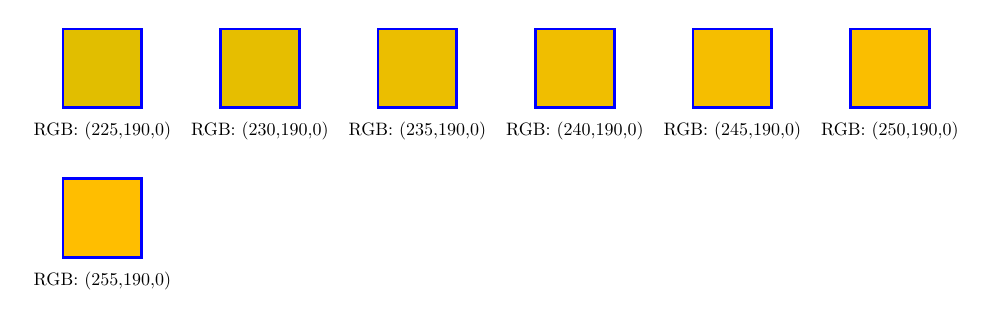
\begin{tikzpicture}

    \filldraw[draw=blue,line width=1,fill=colorR225G190B0]
    (0,0) rectangle (1,1);

    \node[scale=0.65] at (0.5,-0.3) {RGB: (225,190,0)};



    \begin{scope}[xshift=2cm]

      \filldraw[draw=blue,line width=1,fill=colorR230G190B0]
      (0,0) rectangle (1,1);

      \node[scale=0.65] at (0.5,-0.3) {RGB: (230,190,0)};

    \end{scope}



    \begin{scope}[xshift=4cm]

      \filldraw[draw=blue,line width=1,fill=colorR235G190B0]
      (0,0) rectangle (1,1);

      \node[scale=0.65] at (0.5,-0.3) {RGB: (235,190,0)};

    \end{scope}



    \begin{scope}[xshift=6cm]

      \filldraw[draw=blue,line width=1,fill=colorR240G190B0]
      (0,0) rectangle (1,1);

      \node[scale=0.65] at (0.5,-0.3) {RGB: (240,190,0)};

    \end{scope}



    \begin{scope}[xshift=8cm]

      \filldraw[draw=blue,line width=1,fill=colorR245G190B0]
      (0,0) rectangle (1,1);

      \node[scale=0.65] at (0.5,-0.3) {RGB: (245,190,0)};

    \end{scope}



    \begin{scope}[xshift=10cm]

      \filldraw[draw=blue,line width=1,fill=colorR250G190B0]
      (0,0) rectangle (1,1);

      \node[scale=0.65] at (0.5,-0.3) {RGB: (250,190,0)};

    \end{scope}







    \begin{scope}[yshift=-1.9cm]

      \filldraw[draw=blue,line width=1,fill=colorR255G190B0]
      (0,0) rectangle (1,1);

      \node[scale=0.65] at (0.5,-0.3) {RGB: (255,190,0)};

    \end{scope}

  \end{tikzpicture}

  \caption{Mixed colors in~RGB system: $(225,190,0)$--$(255,190,0)$}



  \label{fig:Mixed-colors-Part-10}

\end{figure}
% ##################










% ####################################################################
% ####################################################################
% Bibliography

% \printbibliography





% ############################
% End of the document

\end{document}
